\documentclass[oneside,12pt]{book}

% Package dependencies
\usepackage{geometry}
\usepackage{lipsum}
\geometry{left=32mm, right=30mm, bottom=25mm, top=25mm}
\usepackage{amsmath , amsthm , amssymb}
\usepackage{float}
\usepackage{hyperref}
\usepackage{apacite}
\usepackage{scrextend}
\usepackage{blindtext}
\usepackage{fancyhdr}
\usepackage{multicol}
\usepackage{csquotes}
\usepackage{bm}
\usepackage{subcaption}
\usepackage{tocbibind}
\usepackage{pdfpages}
\usepackage[toc,page]{appendix}
\usepackage{wrapfig}
\usepackage{colortbl}
\usepackage{multirow}
\usepackage{listings}
\usepackage[font=scriptsize]{caption}

% document formatting
\addtokomafont{labelinglabel}{\sffamily}
\setlength{\columnsep}{1cm}
\renewcommand{\baselinestretch}{1.5}

\lstdefinelanguage{JavaScript}{
  keywords={break, case, catch, continue, debugger, default, delete, do, else, finally, for, function, if, in, instanceof, new, return, switch, this, throw, try, typeof, var, void, while, with},
  morecomment=[l]{//},
  morecomment=[s]{/*}{*/},
  morestring=[b]',
  morestring=[b]",
  sensitive=true
}

\lstset{
  basicstyle=\ttfamily,
  columns=fullflexible,
  frame=single,
  numbers=left,
  stepnumber=1,
  breaklines=true,
  postbreak=\mbox{\textcolor{red}{$\hookrightarrow$}\space},
}


\begin{document}

% Title page
\begin{titlepage}
    \begin{center}
        \vspace*{1.5cm}
        \Huge
        \textbf{Performance comparison between a distributed particle swarm algorithm and a centralised algorithm}
        
        \vspace{0.5cm}
        \begin{figure}[H]
    	\centering
    	\hspace{7mm} \includegraphics[scale=0.5]{TU_logo}
        \end{figure}
        
        \vspace{1.5cm}
        
        \textbf{Ciarán O'Loughlin}
        
        \vfill
       \large
        A dissertation submitted in partial fulfilment of the requirements of\\
	Dublin Institute of Technology for the degree of\\
	M.Sc. in Computing (TU060)\\
       \vspace{0.5cm}
        \textbf{Date}
        \vspace{0.8cm}
 
    \end{center}
\end{titlepage}

% Define headers / footer style for the whole doc
\pagestyle{fancy}
\fancyhf{}
\fancyfoot[CE,CO]{\thepage}
\renewcommand{\headrulewidth}{0pt}

% APA style for referencing
\bibliographystyle{apacite}

% Roman numerals for the 'administrative' sections
\pagenumbering{Roman}

% Declaration page
\chapter*{Declaration}
\addcontentsline{toc}{chapter}{Declaration}
I certify that this dissertation which I now submit for examination for the award of
MSc in Computing (Stream), is entirely my own work and has not been taken
from the work of others save and to the extent that such work has been cited and
acknowledged within the text of my work.
\\
\\
This dissertation was prepared according to the regulations for postgraduate study of
the Dublin Institute of Technology and has not been submitted in whole or part for an
award in any other Institute or University.
\\
\\
The work reported on in this dissertation conforms to the principles and requirements
of the Institute’s guidelines for ethics in research.
\vfill
\noindent
\textit{\textbf{Signed:}}  \\

\noindent
\textit{\textbf{Date:}}
\vspace{0.8cm}

% Abstract
\chapter*{Abstract}
\addcontentsline{toc}{chapter}{Abstract}
\par 
Particle Swarm optimisation(PSO) is a particular form of swarm intelligence, which itself is an innovative intelligent paradigm for solving optimization problems. PSO is generally used to find a global optimum in a single optimisation function. This typically occurs on one node(machine) but there has been a significant body of research into creating distributed implementations of the PSO algorithm. Such research has often focused on the creation and performance of the distributed implementation in an isolated manner, or compared to different distributed algorithms. 

This research piece aims to bridge a gap in the existing literature, by testing a distributed implementation of a PSO algorithm against a centralised implementation, and investigating what, if any, gains there are, to utilising a distributed implementation over a centralised implementation. The focus will primarily be on the time to solution aspect of the algorithm, but other elements will be examined over the course of the study.  

\vfill
\noindent
\textbf{Keywords:} \quad Swarm Intelligence, Particle Swarm Optimisation, PSO, Distributed Algorithms

%Acknowledgements
\chapter*{Acknowledgments}
\addcontentsline{toc}{chapter}{Acknowledgments}

I would like to express my sincere thanks to my supervisor Dr. Edina Hatunic Webster, whose guidance, and support helped me throughout my dissertation. 

\vspace{5mm}

{\setlength{\parindent}{0cm}A special thanks to my parents Eileen \& Cormac O'L., my friends, colleagues and family. Without all their encouragement and support this dissertation would never have been possible.}

% Contents and lists
\newpage
\tableofcontents

\listoffigures

\listoftables

\lstlistoflistings

\chapter*{List of Acronyms}
\addcontentsline{toc}{chapter}{List of Acronyms}
\begin{table}[H]
  \centering
    \begin{tabular}{ l l }
    \textbf{PSO} & Particle Swarm Algorithm \\
    \textbf{LTS} & Long Term Support \\
    \textbf{CPU} & Computer processor unit \\
    \textbf{RAM} & Random Access Memory \\
    \textbf{TTS} & Time To Solution \\
    \textbf{CSV} & Comma Separated Values \\
    \textbf{JSON} & JavaScript Object Notation \\
    
    \end{tabular}
\end{table}

\newpage

% Standard numbering starts from here
\pagenumbering{arabic}
\fancyhead[RE,LO]{\leftmark}
\renewcommand{\headrulewidth}{2pt}


% Start of core thesis content

%Introduction chapter
% ============================================================= %
\chapter{Introduction}
\section{Background}
\par Swarm Intelligence (SI) is an innovative distributed intelligent paradigm for solving optimization problems that originally took its inspiration from the biological examples by swarming, flocking and herding phenomena in vertebrates \cite{abraham_guo_liu_2006}.
Within the boundaries of swarm intelligence there are many different algorithms, all with different uses and capabilities. One particular algorithm is the Particle swarm optimisation algorithm(PSO). PSO is a population-based search algorithm and is initialized with a population of random solutions, called particles \cite{shi_2004}. Particles are then arranged into a "swarm". Swarms allow the sharing of information between particles, the so called "social" element of the algorithm. Particle swarm optimisation as an algorithm was first proposed by James Kennedy  and Russell Eberhart in their 1995 paper "Particle Swarm Optimization" \cite{kennedy_eberhart_1995}. While not a new technique, PSO is still being expanded upon today, with modern uses ranging from simple algorithmic evaluation, to more complex robotics implementations. 

This is the basis of a single swarm PSO. However it is possible to increase the number of particles in a swarm, but we can also increase the number of swarms. A multi swarm PSO(Or a Cooperative Particle Swarm Optimisation algorithm, CPSO) model allows for "a significant increases in the solution diversity in CPSO-S algorithm, because of the many different members from different swarms" \cite{vandenbergh_engelbrecht_2004}. Even when using a multi swarm model, there will be hard limits on the number of particles and swarms a singular machine can generate. This is where a distributed model can help, with swarms being logically segregated across a network of machines.

\section{Research Project/problem}
There is an upper limit to the amount of particles any one system can support in a PSO algorithm. At a certain point the algorithm will slow down and the time taken for it to complete an iteration will drastically increase. This will be exacerbated by running multiple swarms. 
To alleviate this problem we can distribute the swarms onto different machines, which allows us to increase the total number of swarms and particles available to us. However, this has a disadvantage as to evaluate results generated by the swarms network communications will need to be established. Network connections are inherently slower than connections and data transfers on a local machine, so the question this report aims to answers is

\textit{"At what point are performance gains in running a particle swarm optimisation algorithm in a distributed environment outweighed by the time lost in network communications between multiple swarms?"}

\section{Research Objectives}
The key objective  of  the  research  is  to  identify  whether  there exists a point whereby its more efficient to run a particle swarm optimisation algorithm in a distributed manner over a centralised manner. To answer this question the following research objectives where identified:
\begin{enumerate}
\item Create a distributed and a centralised implementation of the PSO
\item Generate a result set for the centralised implementation, with varying inputs(Example; different evaluation function, number of swarms and or particles etc.). Average out results with the same inputs
\item Generate a result set for the distributed implementation, with varying inputs(Examples; different evaluation function, number of swarms and or particles etc.). Average out results with the same inputs
\item Cross comparison between the two results sets. Identify points at which distributed had a faster response time, or other values that would make it preferable to  a centralised implementation
\item Identify any limiting factors, significant points of interest in the data and identify future research
\end{enumerate}


\section{Research Methodologies}
The research can be classified based in a few different ways -
\subsection{Based on Type: Primary vs Secondary}
Primary research refers to a collection of original data, specific to a particular research question generated during the project. When doing primary research, the researcher gathers information first-hand rather than relying on available information in databases and other publications.\cite{bouchrika_2020}

Secondary research instead focus's on collecting and summarizing existing data collections and results. This involves researching existing literature, published articles and analyzing the data produced from these articles to come to a new conclusion, or test a hypothesis. When doing secondary research, researchers use and analyze data from primary research sources.\cite{bouchrika_2020}

The research type for this project can be defined as primary research. Data sets needed to answer the research question will be generated during the course of the project. The data set will be unique, as no other study has sought to compare implementation types of particle swarm optimisation algorithms. 
\subsection{Based on Objective: Quantitative vs Qualitative}
Quantitative research methods refer to collecting numerical data, data that can be used to measure variables, predict outcomes etc. Quantitative data is structured and statistical, using a grounded theory method that relies on data collection that is systematically analyzed. Quantitative research is a methodology that provides support when you need to draw general conclusions from your research and predict outcomes.\cite{mcleod_2019}

Qualitative research is the fundamentally opposite to Quantitative research, as it relies on non-statistical and unstructured or semi-structured. It is a methodology designed to collect non-numerical data to gain insights. It relies on data collected based on a research design that answers the question “why.”\footnote{\url{https://www.surveymonkey.com/mp/quantitative-vs-qualitative-research/}}

The research objective of this project can be defined as quantitative research. This study will generate and examine structured data sets, comparing two particle swarm optimisation implementations, and drawing conclusions from those comparisons. 
\subsection{Based on Form: Exploratory vs Constructive vs Empirical}
Exploratory research refers to when researching a problem which has not been clearly defined. Through exploratory research we can determine the best research design and data collection method. 
When conducting constructive research a completely new approach, theory or model will be proposed. Constructive research adds a new contribution to the current body of research. 
Empirical research is a way of obtaining knowledge through direct observation or experience. Empirical research involves a process, of defining a hypothesis, and then making predictions that can be tested using a suitable scientific experiment. 

The study can be defined as an empirical study. This study will define its hypothesis, test that hypothesis, examine the results from tests, and draw conclusions/predictions from the data. Based on that data the hypothesis can then be accepted or rejected, concluding the study.  

\subsection{Based on Reasoning: Deductive vs Inductive}
% Needs rewriting. :(
Deductive reasoning is a basic form of valid reasoning. Deductive reasoning, or deduction, starts out with a general statement, or hypothesis, and examines the possibilities to reach a specific, logical conclusion
Inductive reasoning is the opposite of deductive reasoning. Inductive reasoning makes broad generalizations from specific observations. Basically, there is data, then conclusions are drawn from the data. 

For this study deductive reasoning will be used. The study will state a hypothesis, and attempt to validate that hypothesis testing, generating data sets and drawing conclusions from those data sets. 

\section{Scope and Limitations}
The scope of this research is to identifier potential points where a distributed implementation of the particle swarm optimisation algorithm is faster than a centralised implementation. 

There are two main limiting factors to this research. The first being that the implementations are only tested against specific fitness functions. There are many different fitness functions, or optimisation problems, that can be applied to a particle swarm optimisation algorithm, and many of them will have different efficiency points, some may gain a benefit from being distributed at different levels of swarms and particles, and others may not ever benefit from being distributed. For this reason three different algorithms where chosen and tested against the two implementations. 

The second limiting factor is an environmental one. Computers with better quality CPU(Computer processor unit) and a higher amount of RAM(Random Access Memory) will be able to support more swarms and particles. In order to account for this the same machine type will be used across the distributed and non distributed implementations. How this will be achieved is discussed in chapter three, Design and Implementation Overview. 

\section{Document Outline}
%Needs Rewritting, just place holder
\subsubsection{Chapter one}
Chapter one is a short introduction and few reasons why this research was conducted.
\subsubsection{Chapter two}
Chapter two involves a comprehensive literature review. Some gaps in the existing research  are discussed.
\subsubsection{Chapter three}
Chapter three includes a detailed design of the experiment as well as the methodology behind it. The design of the testing systems and some implementation overviews are presented. 
\subsubsection{Chapter four}
Chapter four contains a full discussion of the implementation details. Coded examples are provided to add further clarity to how the experiment was built. Environment and test implementations are also discussed. 
\subsubsection{Chapter five}
Chapter five presents the results obtained from running the experiment. Some observation and discussion is presented around these results. 
\subsubsection{Chapter six}
Chapter six is a final discussion and conclusion of the research project, including future suggestions on the given problem as well as recommendations regarding accuracy of the experiment and its design

% Literature review chapter
% ============================================================= %
\chapter{Background Research}
\section{Introduction}
This  chapter  provides  a  review of the  literature available on particle swarm optimisation algorithms, distributed implementation, various  approaches adopted  to  solve  the  problem  and  evaluation metrics used  for  evaluating  the results.  The  chapter  concludes with  the  gaps  in  the existing research and forms the objective for the research.
\section{PSO(Particle Swarm Optimisation)}
\subsection{What is PSO?}
The original PSO algorithm was introduced in 1995 \cite{kennedy1995particle}, in the paper they discussed what the PSO algorithm is, and how to use it to optimise nonlinear functions. At its heart PSO is a population based optimization technique where the population is referred to as a swarm, and population members are referred to as particles. At the algorithms inception, a number of unique particles are created and given random positions within a D-dimensional space. Each particle can be considered a potential solution to the fitness function. Particles then go through iterations, or epochs, where each particle calculates its own personal best evaluation value, then the global best value is calculated. Particles are encouraged to move closer to their own personal best or the groups based on the algorithms implementation. A particle moving closer towards the groups best will define a higher "social value", and moving closer to its own personal best will define a higher "cognitive value". Velocity can also be changed to reduce the variance in particle positions between epochs.
\begin{figure}[H]
    \centering
    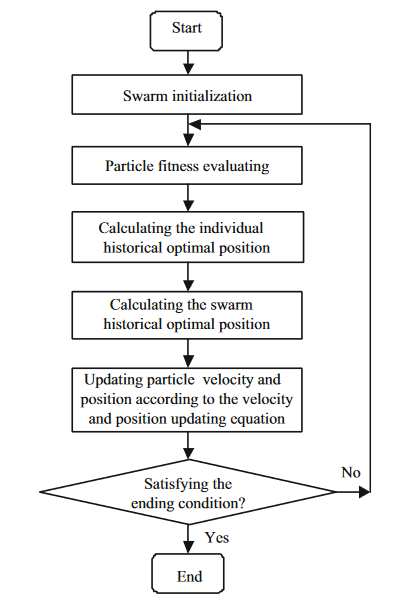
\includegraphics[scale=0.6]{Images/PSO_Flow.png}
    \caption{Flow Diagram of Particle Swarm Optimisation Algorithm \protect\cite{wang_tan_liu_2017}}
    \label{fig:Flow Diagram of Particle Swarm Optimisation Algorithm}
\end{figure}

We can see from the above explanation that PSO shares many elements of other artificial intelligence types, such as evolutionary computation, and genetic algorithms. The particles are manipulated according to the following equations: 
\begin{equation}
V_{id} = W * V_{id} + C_l * Rand( ) * ( P_{id} - X_{id} ) + C_2 * Rand( ) * (P_{gd} - X_{id})
\end{equation}
\begin{equation}
X_{id} = X_{id} + V_{id}
\end{equation}
Where Cl and C2 are two positive constants, Rand() is a random function in the range [0,1], and w is the inertia weight \cite{shi1998parameter}. A particle's new velocity can be calculated using equation 2.1, using its previous velocity and the distances of its current position from its own best experience (position) and the group's best experience. Equation 2.2 calculates the particles new position after its updated velocity. 

\subsubsection{Fitness Function}
When talking about PSO we must also talk about a fitness function. A fitness function is a function that maps the values in particles to a real value that must reward those particle that are closer to the optimisation criterion. Essentially this is the optimisation function to find the minimum or maximum value of. For instance if we wished to find the global minimum of the Beale Function, and optimisation test function we could use PSO. Beale function can be defined as:
\begin{equation}
f(x, y) = (1.5-x+xy)^2+(2.25-x+xy^2)^2+(2.625-x+xy^3)^2
\end{equation}
Using this fitness function the global minimum could be found, in this case it would equate out to be $f(x*)=0$ at $x*=(3,0.5)$ \cite{bingham}. Its important to note that as PSO is a heuristic algorithm, its solution results are not necessarily optimal. PSO will find an answer to a fitness function, but it may not be the best answer to the function. In addition, some problems may have multiple global minimum values, in which case the PSO can only find one answer at a time.

\section{PSO Implementations}
Since James Kennedy and Russell Eberhart original paper there has been significant research into the original algorithm \cite{piotrowski_napiorkowski_piotrowska_2020, bai_2010, imrantextordfeminine2013overview, wang_tan_liu_2017} its applications \cite{hereford_2006, beni_2005, blum_li, raquel2005effective} and its performance \cite{yin_yu_wang_wang_2006, kennedy_1999}. There is also a large body of research into the use of swarm algorithms in distributed environments \cite{akat_gazi_2008, salza_ferrucci_2019, peleg_2005} and centralised environments \cite{trelea_2003, xie2003overview, poli2007particle}, which will be discussed more in the following section. PSO has also been improved upon, with some newer implementations updating the topology or some other underlying principle of the algorithm, examples including SPSO, APSO, TRIBES, Cyber Swarm etc \cite{zhou2009gpu, oca_stutzle_birattari_dorigo_2009, cooren2009performance, yin2010cyber}.

In terms of implementing PSO there have been multiple studies into the uses of swarm intelligence in robotics system \cite{sa_nedjah_mourelle_2016, meng_gan_2008, hereford_2006}. Some other studies also look at interesting use cases PSO and swarm intelligence can be applied to, such as scheduling systems and analysis of distributed systems \cite{li_yang_su_lu_yu_2019, moradi_fotuhi-firuzabad_2008, nouiri_bekrar_jemai_niar_ammari_2015, sahin2007fault}. 

\subsection{Stopping Criteria}
When utilising the PSO algorithm, it is important to identify how and when the algorithm should termninate. The most simple form of stopping criteria is implementing a max number of iterations/epochs check. This is a simple stopping criteria, however it carries with it a risk of stopping the algorithm before a global optimum value has been found. It also must be predefined prior to the algorithms inception, which leaves little leeway for change during runtime.

An alternate to this approach is a check for "when the chance of achieving significant improvements in further iterations is extremely low" \cite{bassimir2020self}. Effectively this is checking to see when the particles are no longer actively moving in the search space, when they have settled at a particular answer. Within the literature there has been some research into more adaptive stopping criteria, for example Zielinski and Laur 2007 paper \cite{zielinski2007stopping}. In this paper a list of upper limit-based and adaptive termination criteria is presented and tested against a real world problem, "optimizing a power allocation scheme for a Code Division Multiple Access (CDMA) system"\cite{zielinski2007stopping}. Both of these approach's offer a more dynamic and adaptive method of stopping the algorithm than the more straightforward maximum iteration check criteria. 

\subsection{Parameter Selection}
As mentioned in earlier sections, there are multiple input parameters for any PSO algorithm, the basic ones being inertia, cognitive and social weightings. Parameters are usually tuned for individual optimisation functions, but there are some basic selecting parameters that are normally used. When looking at the inertia weighting, according to Yan He et al. inertia should be kept within the following range \(w_{min} = 0.4, w_{max} = 0.9\) \cite{he2016parameters}.
When it comes to both cognitive and social weightings, there is a little less consensus, with some research saying both values should be equal to 2 \cite{kennedy_eberhart_1995}, and other literature mentioning that the values should range between 1 and 3 \cite{ZHANG20143576}. It is also suggested that the sum of these constants should not exceed 3 \(i.e s+c \leq 3\) \cite{kan2012convergence}. What is conclusive across all the literature is that each optimisation problem will require its on fine tuning with all three values. 

\subsection{Topology adjustments}
Since its original inception, several adjustments have been proposed in literature to alter some implementation details around PSO. One reoccurring change is a change to the population topology or sociometry. It is well established that these factors play an important role in improving the performance of population-based optimization algorithms by enhancing population diversity when solving multiobjective and multimodal problems \cite{LYNN201824}. Global version PSO (GPSO) and local version PSO (LPSO) are two common neighbor topologies. 
\subsubsection{G-PSO}
In  the  gbest  population,  the trajectory  of  each  particle’s  search  is  influenced  by  the best point found by any member of the entire population\cite{kennedy2002population}. What this means is that the particle uses its experience (the best position achieved so far), and uses the knowledge of the best particle in the swarm to influence its movement strategy. It prioritises the global best value when updating its position.  However, the drawback of this approach is that if the best particles is far  from global optimum, the  swarm can  be  trapped in  local optima since the swarm cannot explore other areas in the search space \cite{azab_hady_hefny_2016}

\subsubsection{L-PSO}
The  lbest  population  allows  each  individual  to  be  influenced  by  some  smaller  number  of  adjacent  members  of the  population  array. Typically  lbest  neighborhoods comprise exactly two neighbors, one on each side: a ring lattice.\cite{kennedy2002population}. The same update function is used by particles in the two topologies, however lbest is generally considered to be the slower topology. Its advantage is that it's much less likely to get stuck in the local optima, and therefore finds the target value far more frequently. 

\begin{figure}[H]
    \centering
    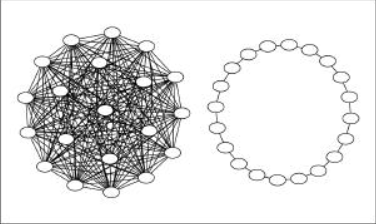
\includegraphics[scale=1.0]{Images/NeighborhoodTopology.png}
    \caption{GBest(Left) and LBest(Right) sociometric patterns.\protect\cite{kennedy2002population}}
    \label{fig:GBest(Left) and LBest(Right) sociometric patterns.}
\end{figure}

\subsection{Multi Swarm PSO}
As mentioned previously there has been a wide body of research conducted into variants of the original PSO algorithm. One such area has been in using multiple swarms, with researches finding some success with their implementations. One such implementation is the MSPSO(multi-swarm particle swarm optimization).  MSPO "\textit{is based on multiple swarms framework cooperating with the dynamic sub-swarm number strategy (DNS), sub-swarm regrouping strategy (SRS), and purposeful detecting strategy (PDS)}" \cite{XIA2018126}. Using these strategies allows MSPSO to balance its exploration and the exploitation ability, resulting in good performance, in terms of solutions accuracy. It however does suffer from an increased time complexity when compared to several other PSO implementations. 
IPSO(Improved  particle  swarm  optimization   algorithm) is another mutli swarm technique that "\textit{adopts   a   new   mutation  operator  and  a  new  method  that  congregates  some  neighboring  individuals  to  form  multiple  sub-populations  in  order  to  lead  particles  to  explore  new  search space}" \cite{zheng2007improved}. Subdividing out the population into multiple neighborhoods, or swarms allows the algorithm to divide up the problem space, and thereby improve performance. Utilising the mutation factor also allowed the implementation to "\textit{enhance the efficiency of advantageous direction of flying particles, so particles can fly to feasible region more quickly and more efficiently}".
\begin{figure}[H]
    \centering
    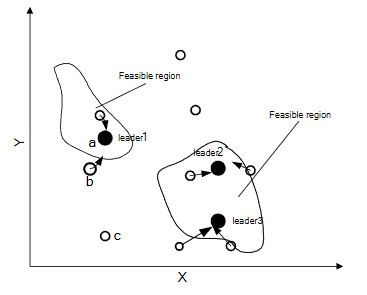
\includegraphics[scale=1.0]{Images/IpsoFormingSwarms.png}
    \caption{IPSO multi-populations being formed .\protect\cite{zheng2007improved} }
    \label{fig:IPSO multi-populations being formed.}
\end{figure}

\subsection{Distributed PSO}
\subsubsection{dPSO}
As mentioned in chapter one, there will be a limit to the number of particles and swarms any one computer can support, the limiting factor being the amount of memory or computational power. To avoid this bottle neck there has been a significant body of research into creating a distributed implementation of the PSO algorithm.  One such area of research is in robotics, using PSO as a search algorithm distributed across many particles, in reality acting as particles in the PSO. In James M. Hereford paper, "\textit{A Distributed Particle Swarm Optimization Algorithm for Swarm Robotic Applications}" a distributed PSO algorithm is proposed, which he calls the dPSO \cite{hereford_2006}. Listing 2.1 shows the pseudo code used to implement the algorithm. 

\begin{lstlisting}[language=inform, caption=Herefords dPSO Code Flow]
pbest = -1; gbest = -1; % Initialize pbest and gbest 
While (target not found or time not expired) 
	% Make measurement and update, if necessary 
    meas = make_measurement();  
    if (meas > pbest) % Update pbest, if true
    	Up_pbest(); %Update pbest value and location
        if (meas > gbest) % Update gbest, if true
        	Set gflag; % set a flag 
            Up_gbest(); %Update gbest value and location
        end 
     end 
     Move(); % Move bot based on PSO update equation  
     % For simulation, constrain bot movement 
     % Two conditions: 
     %   (1) Magnitude of velocity must be < Vmax 
     %   (2) Direction must be within in max turn angle
     If (new gbest found) %broadcast new gbest value       
     	Broadcast(gbest);  
     end
     If (gbest is global gbest) %broadcast gbest location      
     	Broadcast(gbest_location);  
     end
  End while
\end{lstlisting}

In the paper Hereford designed the algorithm for robotic operators, using search algorithms to find specific targets within a search space. From the pseudo code we can see that once a new global best has been found by an operator, that best value is broadcast to all particles in the swarm. 
This creates a truly distributed model, with no reliance on a central operator to process the results of all the particles. Particles must maintain an active list of all particles in the swarm, in order to broadcast the new global best value. So if a new particle(robot) is added to the swarm, all particles must be updated to be made aware of that new particle. 
In his results he found a good deal of success, with the robots finding there target 99\% of the time. Additionally he found that as you increase the number of particles in the swarm the time to find the solution considerably reduces. 
\begin{figure}[H]
    \centering
    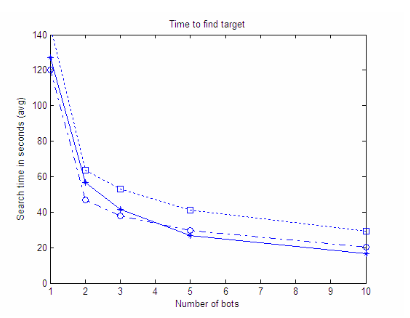
\includegraphics[scale=0.9]{Images/HerefordResults.png}
    \caption{dPSO Time to find Target \protect\cite{hereford_2006} }
    \label{fig:dPSO Time to find Target}
\end{figure}

\subsubsection{AGLDPSO}
In Wang et als. paper "Adaptive Granularity Learning Distributed Particle Swarm Optimization for Large-Scale Optimization" a distributed implementation is proposed, called AGLDPSO(Adaptive granularity learning distributed particle swarmoptimization) \cite{wang2020adaptive}. AGLDPSO uses a master-slave relationship when creating distributed particles, which is significantly different to Herefords distributed model, whereby all particles are peers within a swarm, there is no orchestration or master controller. Each particle, or robot was aware of all other robots in the swarm and updated accordingly. In AGLDPSO, a master acts as the intermediary and updates all particles in the population. This works very well for their implementation, but creates a network bottle neck that dSPO altogether avoids. When tested against multiple other optimisation algorithms the authors found that AGLDPSO "\textit{achieves a promising and satisfying performance when solving the large-scale optimization problems.}". 
\begin{figure}[H]
    \centering
    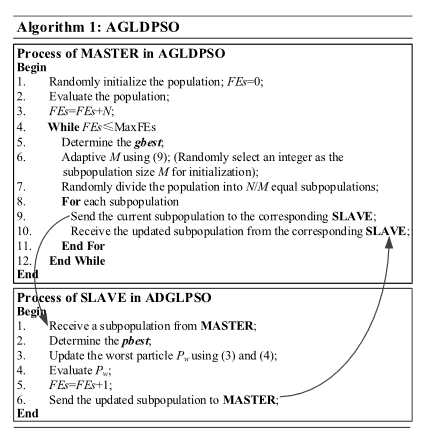
\includegraphics[scale=0.8]{Images/AGLDPSO.png}
    \caption{Flow Diagram of AGLDSPO \protect\cite{wang2020adaptive} }
    \label{fig:Flow Diagram of AGLDSPO}
\end{figure}

\section{Evaluating performance}
\subsection{Benchmarking}
Benchmarking, also referred to as "best practice benchmarking" or "process benchmarking", is  a  method  of  conducting  necessary  actions  and  activities  in  order  to evaluate  how  a  given  piece  of  software  or  a  system  is  going  to perform  once  it  is deployed and used in the field \cite{vokolos1998performance}. When speaking of software performance we general refer to throughput, stimulus, response time, or some combination of the two\cite{vokolos1998performance}.  It is also a way of assessing the system’s availability. Meaning that whenever the system undergoes high levels of stress, be it increasing the number of processed requests (throughput), or high resource consumption (machine resources), the system still processes these requests or events in acceptable numbers\cite{vokolos1998performance}.  Usually benchmarking involves predicting how a technology will behave once its used in regular every day life, for instance benchmarking a web server will allow organisations to predict how well it will cope with increased web traffic. The predictions allow organisation to anticipate potential limitations, and can lead the organisation to a plan to overcome those limitations. Utilising a benchmarking evaluation strategy the study will compare the two proposed PSO implementations, providing insights into the performance of a distributed implementation. 
 
\section{Research Gaps}
As outlined above there has been a large amount of research in the area of Swarm intelligence over the past 20 years. We can see in J. F. Schutte et. al article they had a comprehensive cover of using parallel PSO \cite{schutte2004parallel}, however to limit network connection time the used a parallel processor for running the algorithm. This would certainly cut down on networking connection times, however it can not be described as a truly distributed algorithm. S. Burak Akat and Veysel Gazi focused much more on the distributed aspect of the algorithm, but no effort was made at running comparisons between the distributed version and a non distributed version of the algorithm \cite{akat_gazi_2008}. James M. Hereford again focused on the distributed aspect of the algorithm, with no relative benchmarks comparing it to a non distributed version. \cite{hereford_2006}

The gap identified for this research is the performance benefits of running a PSO algorithm in distributed environments vs centralised environments. As you can see from the above there has been plenty of research into crafting and testing distributed implementations of the PSO algorithm, but there has been no published literature testing the PSO algorithm in distributed environments vs a centralised environments and comparing the results, with an emphasis on finding a point where a distributed implementation is more time efficient than a centralised implementation. 

\section{Conclusion}
In this chapter an overview of PSO was presented, along with some more in depth research into parameter selection and different PSO implementations where discussed. Multi swarm PSO was discussed at a high level and two distinct distributed PSO implementations where presented and discussed.
Research gaps where identified and discussed, along with the evaluation metric that will be used in this study. 

The next chapter will focus on the experiment design and methodology. It will also cover the aim of the research and provide a basic overview of the experiment implementation details.


% Design and methodology chapter
% ============================================================= %
\chapter{Experiment design and methodology}
\section{Introduction}
This chapter presents the design used to craft the experiment and the methodologies used to test the results from that experiment. The chapter will cover the aim of the research, the design and implementation of the experiment, data output design and will conclude with design conclusions. 
\section{Aim of Research}
The aim of this paper is to find out if a point exists when scaling a PSO algorithm, that it becomes more efficient to run a distributed algorithm instead of a centralised algorithm. Increasing the number of active particles in a PSO algorithm can lead to a decline in performance, as for each iteration or epoch the machine must dedicate more and more computational power to recalculate particles positions and best evaluations. In a distributed model this burden can be divided across a number of machines, however in order to calculate the global best value network communications must occur between machines, thus forming the swarm. Network communications are inherently slower than local connection communications, however at high levels of active particles this speed decrease may be alleviated by the increased computational power available. 

\section{Hypothesis}
\subsubsection{Null Hypothesis H\textsubscript{0}:}
The time taken to find a stabilised result from using a distributed network of swarms never exceeds the time lost from the network communications needed to update swarms of each others presence and activities.

\subsubsection{Alternate Hypothesis H\textsubscript{1}:}
The increased speed to solution time from using a distributed network of swarms exceeds the time lost from the network communications needed to update swarms of each others presence and activities once the number of particles and/or swarms has reached a sufficient level.

\section{Design overview}
In order to create the data required to prove/disprove the hypothesis two code base's will need to be created. One code base will need to handle generating the data required for a centralised PSO,and the other will need to generate the data from a distributed PSO implementation. Each will need to be able to run the same fitness functions, and operate nearly identically, except the distributed implementation, which will need to call other PSO nodes to run swarms rather than running them on the local system. 
The coded system will need to be run multiple times with the same inputs in order to account for the random element inherit in the PSO algorithm. After each run the system will need to output all generated data, and a data aggregator will need to sort, average and output all the data in order for it to be evaluated.

\begin{figure}[H]
    \centering
    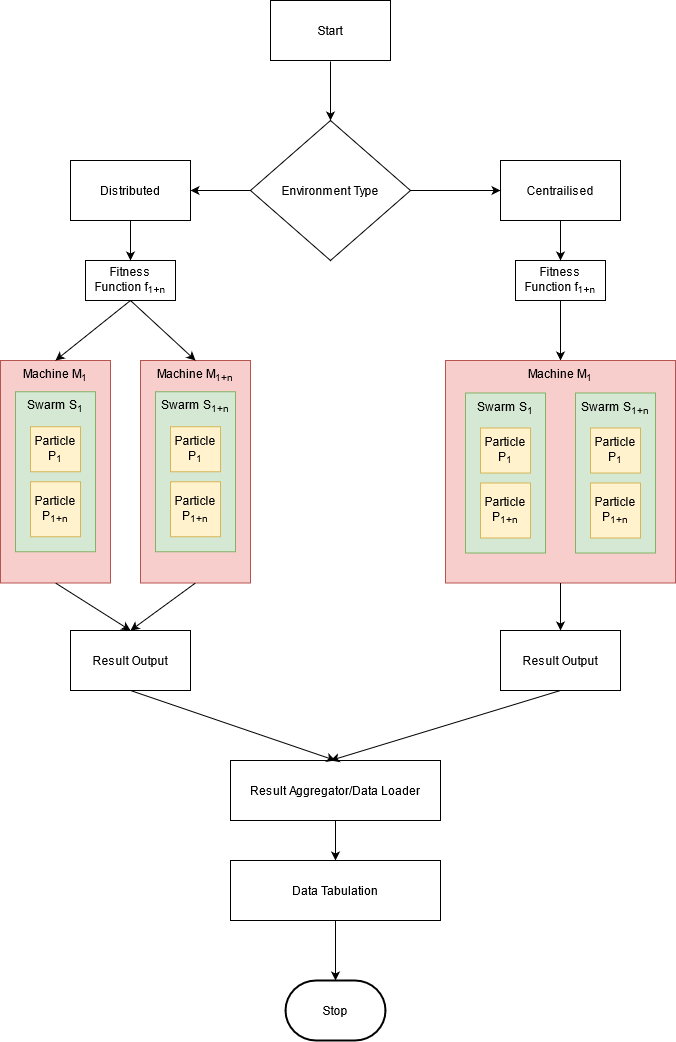
\includegraphics[scale=0.6]{Images/ExperimentFlow.png}
    \caption{Experiment Design Flow Chart}
    \label{fig:Experiment Design Flow Chart}
\end{figure}
Figure \ref{fig:Experiment Design Flow Chart} displays the flow of the experiment. First the environment type will be chosen, then from that point the required fitness function will be chosen. To give greater breath to the results three different fitness functions will be used, with varying degrees of complexity. Once the fitness function has been chosen, the swarms and particles can be initialised with the function implementation. In the case of the centralised implementation this will be the same machine, in the decentralised implementation swarm nodes will be contacted and initialised. Once each environment type has completed its run and found a stable answer the implementations will return a data response object. 

At this point the data aggregator will pull in the results from both implementations, with corresponding configuration details and generate a data output file useful for data comparison. This data file will be loaded into a data tabulation tool, whereby the results can be inspected and comparisons can be drawn up. At this point the study will be able to draw conclusions on whether the alternate hypothesis can be accepted or rejected.  

\subsection{Centralised PSO Design}
Expanding on the design overview, the centralised implementation will need to perform several steps in order to generate the required results set. Firstly it will initialise and create a parameterised number of swarms, each with a parameterised number of particles. At this point the first iteration will begin for all swarms. This will all occur on the one node. The iteration will follow the same format as what was discussed in section 2.2.1. Each swarm will attempt to find its group best value. All swarms will then report the group best value. At this point the controller class, which will also be the class that instantiates the swarms, will try and calculate if a "settled" group best value has been found. What this means is that at a certain point the algorithm will settle on a particular value, the global minimum. This will be the optimum solution to the fitness function. In this context settled means that for a certain number of iterations the same group best value will be returned across all swarms. So the system will need to record past values and compare against returned values to see if the same value has been returned for multiple iterations in a row. When this has occurred the domain controller will calculate the time to arriving at this optimal solution, and the number of iterations it took to find that value, this being the TTS (Time to solution) value. 
The basic flow of Centralised implementation is shown below in figure \ref{fig:Flow Diagram of Centralised Particle Swarm Algorithm}. 
\begin{figure}[H]
    \centering
    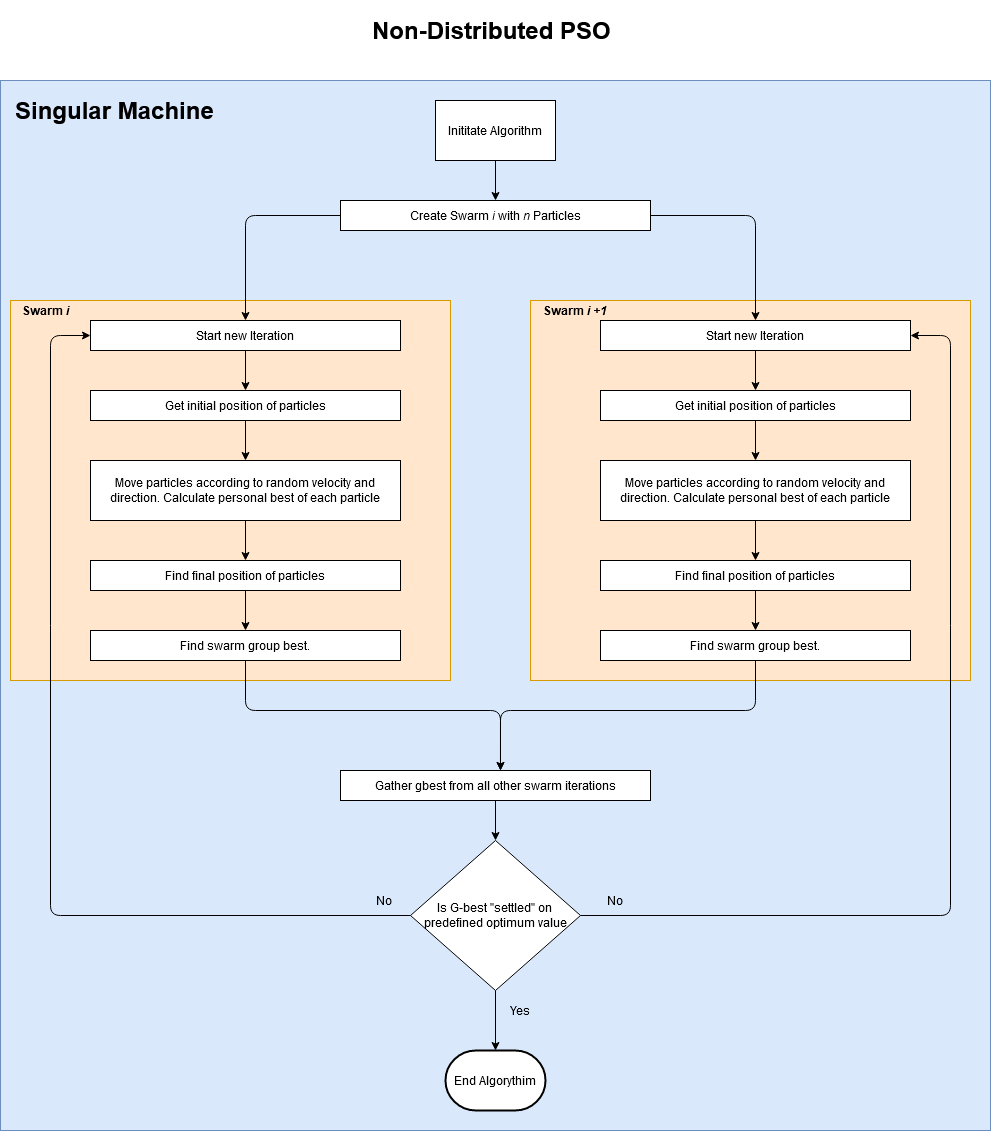
\includegraphics[scale=0.4]{Images/FlowDiagramNonDistibutedPSO.png}
    \caption{Flow Diagram of Centralised Particle Swarm Algorithm}
    \label{fig:Flow Diagram of Centralised Particle Swarm Algorithm}
\end{figure}

\subsection{Distributed PSO Design}
\begin{figure}[H]
    \centering
    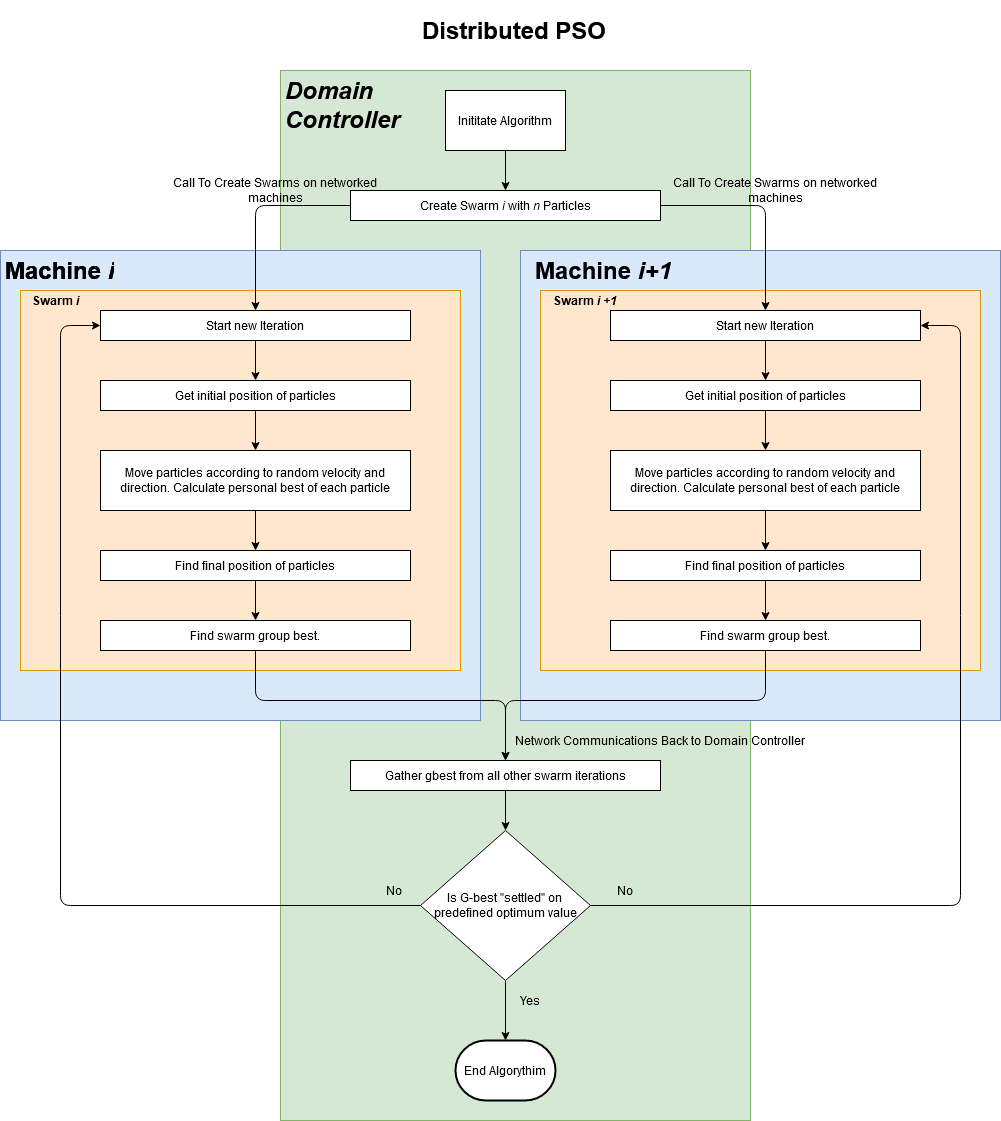
\includegraphics[scale=0.4]{Images/FlowDiagramDistibutedPSO.png}
    \caption{Flow Diagram of Distributed Particle Swarm Algorithm}
    \label{fig:Flow Diagram of Distributed Particle Swarm Algorithm}
\end{figure}
As discussed in the overview, the distributed implementation will function similarly to the centralised implementation to keep differences in results to a minimum. The only functional difference will be that swarms will be logically separated across multiple machines in the distributed implementation. Where the centralised implementation will be running a domain controller, and all swarm instances, the distributed implementation will feature a domain controller on a single node, calling out to other networked nodes, that will startup and iterate individual swarms with a parameterised number of particles. Once an iteration ends the node will communicate back to the domain controller, which will collect responses from all active swarms, and check to see if the swarms have "settled" on the parameterised global minimum value. 
If they have the domain will stop the nodes from running any further iterations, collect resulting values, ie. number of iterations and time to solution. Network time will be accounted for in the time to solution value.

\section{Distributed environment}
In order to create a distributed environment for the distributed implementation for this project a cloud provider was used. Using these cloud providers a virtual machine can be created and initialised, allowing the end user or developer to install custom software and applications. In this instance it allows the distributed implementation and centralised implementation to be deployed and run in a containerised environment. Snapshots where used to ensure consistency between the two implementations, and between the nodes of the distributed implementation. To facilitate this a number of different providers where considered, including AWS(Amazon Web Services), Google cloud and Digital Oceans. Each had a containerised virtual machine product that allowed the deployment of custom applications, along with unique domain names and other internet connection utilities, however only one provider was required and Digital Ocean was chosen as the provider for this project. 

\subsection{DigitalOcean}
Digital Ocean is an Infrastructure as a Service(IaaS) platform for software developers. It allows developers to create containers in a simple and quick manner. To deploy Digital Ocean's IaaS environment, developers launch a virtual machine instance, which DigitalOcean calls a "droplet.". This is containerised, and a number of operating systems can be chosen to initialise the doplet. The OS's available to developer include: Ubuntu, CentOS, Debian, Fedora, CoreOS or FreeBSD. Digital ocean also offer the ability to choose the geographic region the droplet will be created in, and some other configuration options such as the amount of dedicated ram, number/quality of CPU, and the size of the on-board hard drive. Once initialised the developer may install their own custom software, or use some prepared packages from digital ocean to help speed along deployment. 

Once the droplet has been created developers have the ability to monitor activity from their browser using digital oceans control panel. They also have the ability to update the domain name, and create a VPN(Virtual Private Network) for the droplet. Snapshots of the droplet can be taken at any time and used to recreate it if required. Digital ocean is a very affordable option among its peers, with basic containers costing at minimum 0.00744\$ an hour, working out at 5\$ a month. \footnote{https://www.digitalocean.com/pricing} For that price digital ocean provide a container with one gigabyte of RAM, one core CPU and twenty gigabytes of on-board storage.

\subsection{Container and Network Design}
As previously mentioned the distributed provider used for this project will be digital ocean. Utilizing the containerisation service previously mentioned, a number of droplets will be created. Droplets will contain the implementation code in order to act as a domain controller and as a swarm node. However each node will only ever act as a domain controller or a swarm node. This design can be seen in figure \ref{fig:ContainerDesignOverview}. When running the distributed implementation the domain controller node will be called using the same request as the non-distributed method, however instead of an integer defining the number of swarms to be used, a list of IP address will be passed in. These IP address will correspond with the IP address's for the droplets running swarm nodes. The domain controller will then connect with each of these droplets, initialise the swarm node with the passed in configuration values, begin iterating and collecting response from all connected swarm nodes.

\begin{figure}[H]
    \centering
    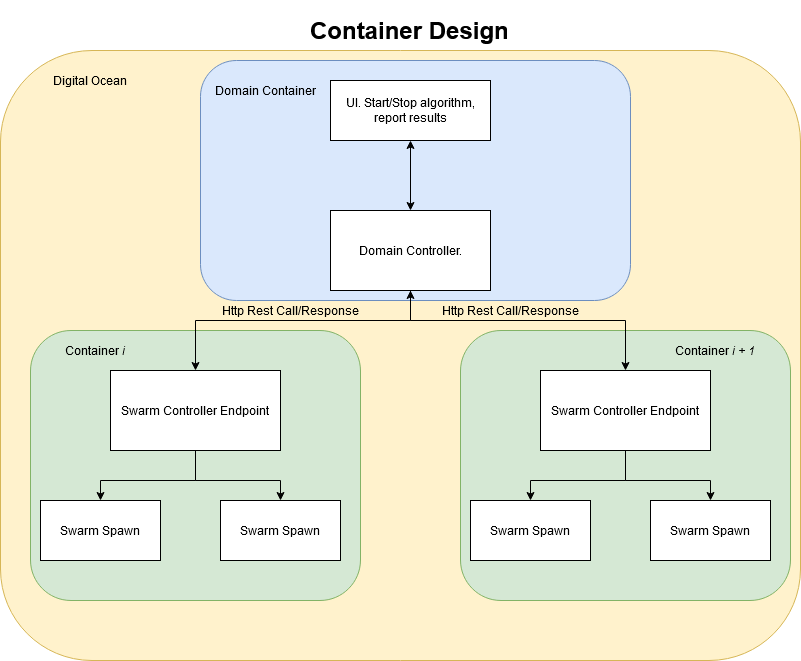
\includegraphics[scale=0.4]{Images/ContainerDesign.png}
    \caption{Container Design Overview}
    \label{fig:ContainerDesignOverview}
\end{figure}

This design does feature a core flaw in that it creates a central dependency in the domain controller. However in order to keep the results as consistent and in line with the centralised implementation, the domain controller will be the same droplet size as all other swarm nodes. 

\section{Data Design and Data Capture Overview}
For the purpose of this project the following variables will be recorded for comparison. 
\begin{table}[H]
  \centering
    \begin{tabular}{| c | c | c |}
    \hline
     & \textbf{Variable Description} & \textbf{Data Type} \\ \hline
    \textbf{Time} & Time taken to get to solution & Integer \\ \hline
    \textbf{N-Particles} & Number of active Particles  & Integer \\ \hline
    \textbf{N-Swarm} & Number of active Swarms. & Integer \\ \hline
    \textbf{Environment-Type} & Distributed or Centralised & String \\ \hline
    \textbf{Iterations} & Total number of iterations to reach a solution & Integer \\ \hline
    \textbf{finalGroupBest} & Final group best from all swarms & Integer \\ \hline
    \textbf{averageBestX} & Average best X value across all swarms  & Integer \\ \hline
    \textbf{averageBestY} & Average best Y value across all swarms & Integer \\ \hline
    \end{tabular}
  \caption{Data output variables}
  \label{tab:data_output_design}
\end{table}
Starting with the first variable in table \ref{tab:data_output_design}, the time variable, this will represent the amount of time it took the specific test to calculate an answer, essentially this is the TTS value. This will be recorded in milliseconds, and it will be calculated by the domain controller, starting from the time it initialise the swarms in either the distributed implementation or the centralised implementation, and ending when either implementation arrives at a settled answer. The number of particles and swarms will be specified in the request when running the algorithm, but will also be recorded as part of the output for ease of comparison of results. Again environment type will be specified in the request, and recorded in the output for comparison. The Iterations variable will be used to record the number of iterations or epochs it took to reach a settled solution. This will also include the defined number of iterations for a result to be considered settled, which will inflate the total number of iterations, however as this affects all test runs it will have no significant impact on the final values. Final group best value will record the final gbest answer. All iterations should come to the same value, as the fitness functions used will contain only one global minimum, however it was recorded to see if there was any variation in the results between implementation types. Similarly with average best x and y all implementations types should conclude with the same values, but they where recorded to see if there was any variation.
This data will be outputted to a JSON(JavaScript Object Notation) file at the end of each test run. The JSON file will be named in the following convention:

\verb|<Function-Name>_<SwarmNumber>_<ParticleNumber>.results.json|


\subsection{Data Aggregation}
As mentioned in section 3.4 Design overview, due to the random element of the PSO algorithm, an average of results with the same parameters will need to be taken. Therefore multiple data output files will be generated for tests with the same inputs. In combination with multiple tests with varied numbers of particles and swarms, a large number of output files will be generated. To deal with this a data aggregation system will need to be created. This aggregation system will load in results with the same input variables, create an average values for the time to solution variable, number of iterations, finalGroupBest, and averageBestX/Y values. Values will then be outputted  into a single data file, with results from the distributed and centralised implementation being directly compared.

\section{Design and Methodology Summary}
This chapter presented an overview of the design and methodology used for this research. It discussed the overarching design of the experiment, with subsequent sections going into a more detailed design of specific elements of the research. Data output and capture was also discussed, with a data output design presented in some detail. 
The next chapter will focus in on the implementation detail, providing coded examples of the design presented in this chapter. 

% Experiment Implementation details(The only fun chapter really) 
% ============================================================= %
\chapter{Experiment Implementation}

\section{Introduction}
This chapter will expand on the previous chapter and cover the implementation details in more depth. Coding examples will be provided for more clarity on how the two PSO implementations function. Additionally the test harness and data loader that where created for this experiment will be expanded upon and coded examples of each will be given.

\section{PSO Implementations}

\subsection{Java}
For the purpose of this study Java will be used as the implementation language. Java is a mature language, with its initial 1.0 release in 1995. Since then its gone through multiple iterations and major version changes. It has been largely adopted by enterprise organisations due to its stability and feature rich ecosystem. Java was chosen due to the "deploy anywhere" model that allows for applications to be run on any operating system that supports a JVM(Java Virtual Machine). This will be a benefit when the application is deployed to a distributed environment. Other advantages of using Java are its quite performant \footnote{https://www.infoq.com/presentations/java-8-13-performance/} \footnote{https://www.toptal.com/back-end/server-side-io-performance-node-php-java-go}, has a large set of supported libraries and extensions, along with a very active community and a wide range of supporting tools and documentation.

\subsection{Spring Boot}
Spring Boot is an open source Java-based framework, that includes many utilities and libraries that allows a developer to quickly create a "production-grade"\footnote{https://spring.io/projects/spring-boot} application and is developed by Pivotal team. Spring boot is configured with an embedded servlet container, contains many auto-configurations features for ease of development, and provides plenty of additional tools for crafting microservices. 

Spring boot was used in this experiment because of its mature and stable nature, and the ability to easily create REST(Representational state transfer) based services. Due to the distributed nature of the experiment, REST API calls where used to facilitate the messaging between swarm nodes and the domain controller. More on this will be discussed in the following sections. Spring boot allows developers to quickly configure REST API's, and is reasonable performant during runtime \footnote{https://spring.io/blog/2018/12/12/how-fast-is-spring}. Spring boot also allows developers to easily configure a number of different logging tools and frameworks to aid in debugging runtime errors and exceptions, which was a requirement during the development phase of this experiment. 


\subsection{Centralised Implementation}
Using spring boot a basic rest controller was created, whereby the swarm could be initialised and run by calling one POST endpoint with a request object that contains the configurable values. Listing \ref{listing:CentralisedRestController} shows the coded example of this. 
\begin{lstlisting}[basicstyle=\footnotesize, language=Java]
@PostMapping("/runSwarm")
public Response runCentralisedSwarm(@RequestBody Request request) throws Exception {
    return centralisedService.runSwarm(request);
}
\end{lstlisting}
\captionof{lstlisting}{Centralised Rest Controller}\label{listing:CentralisedRestController}

Once the endpoint in the rest controller receives a request, it will call out to a service method which will initialise the swarms and particles and begin the running the algorithm. Listing \ref{listing:CentralisedSwarmInitialisation} is an extract of how these swarms are initialised in the service method. The swarm and particle objects are abstracted out of the service class, so that the distributed service class can reuse the same methods, with some modifications. The service class also handles generating the response object with all necessary data points discussed in Chapter three. 

\begin{lstlisting}[basicstyle=\footnotesize, language=Java]
List<Swarm> multiSwarm = new ArrayList<>();
...
/* Initialize all swarms and particle with supplied configuration */
for(int swarmId = 0; swarmId<request.getNumberOfSwarms(); swarmId++) {
    multiSwarm.add(utils.createSwarm(swarmId, request.getNumberOfParticles(), request.getConfigVariables()));
}
\end{lstlisting}
\captionof{lstlisting}{Centralised Swarm initialisation}\label{listing:CentralisedSwarmInitialisation}

Listing \ref{listing:CentralisedIterationMethod} shows an extract of the swarm iteration code in the centralised service. Once the swarms are initialized the service class moves onto iterating through each swarm. We can see in the extract this is done through a while loop. In the while loop each iteration of all swarms is done through a for loop. Each iteration of the while loop counts as a full iteration for all swarms. In the listing we can also see the code records a start time and a stop time. Once completed the time between entering the service class and completing the while loop is calculated. This is used to accurately calculate the time taken only for the PSO code to run, rather than the time to get a response from the rest controller. This is returned as the TTS value. 

\begin{lstlisting}[basicstyle=\footnotesize, language=Java]
Instant start = Instant.now();
...
while(!targetFound) {
    ...
    for(int swarmId = 0; swarmId<request.getNumberOfSwarms(); swarmId++) {
        Result result = utils.runSwarmIteration(multiSwarm.get(swarmId), stepCount);
        ...
    }
    ...
    stepCount++;
}
Instant finish = Instant.now();
long timeElapsed = Duration.between(start, finish).toMillis();
...
\end{lstlisting}
\captionof{lstlisting}{Centralised Iteration Method}\label{listing:CentralisedIterationMethod}

Within the main while loop the code contains the stopping criteria. Listing \ref{listing:CentralisedStoppingCriteria} shows an extract of this code. The code loops through each of the swarms responses and each of their responses are compared to the a previous value, and if the exact same global best has been found for the configured number of times (The \verb|TARGET_NUMBER_OF_EXACT_ANSWERS| variable) then the while loop forcibly ends. This is done through the use of an array list. If th array list is not null, the code checks if the array list contains the current swarms gbest value. If it does, the value is added to the array list, and the code checks the size of the array list, and if its the same as the \verb|TARGET_NUMBER_OF_EXACT_ANSWERS| variable then the while loop ends. If the value isnt present than the array list resets itself to ensure all swarms return the exact same answer the same number of times. If the step count ie. the number of iterations reaches a certain threshold(The \verb|MAX_NUMBER_OF_STEPS| variable) the while loop is also terminated, to prevent the system from becoming trapped in an unending loop. This is assumed to be the worst case scenario, and is not expected to regularly happen. 

\begin{lstlisting}[basicstyle=\footnotesize, language=Java]
/* Check if the same answer has been found multiple times */
for(int swarmId = 0; swarmId<request.getNumberOfSwarms(); swarmId++) {
    if (settledList.size() == 0) {
        settledList.add(bestEvaluation[swarmId]);
    } else {
        if (settledList.contains(bestEvaluation[swarmId])) {
            settledList.add(bestEvaluation[swarmId]);
        } else {
            settledList = new ArrayList<>();
        }
    }
    if (settledList.size() == TARGET_NUMBER_OF_EXACT_ANSWERS) {
        TARGET_NUMBER_OF_EXACT_ANSWERS);
        targetFound = true;
    }
}
\end{lstlisting}
\captionof{lstlisting}{Centralised Stopping Criteria}\label{listing:CentralisedStoppingCriteria}

\subsubsection{Swarm Creation and Initialisation}
Listing \ref{listing:SwarmCreation} has an extract of the swarm creation method. From the method createSwarm we can see how it creates a fitness function based on an enum ("An enum type is a special data type that enables for a variable to be a set of predefined constants" \footnote{https://docs.oracle.com/javase/tutorial/java/javaOO/enum.html}) passed in, allowing for the system to be extended with new fitness functions with a low amount of code change. Fitness function are defined in the request sent into the service, and it initialises the swarm with the number of particles and other configuration values.

\begin{lstlisting}[basicstyle=\footnotesize, language=Java]
public Swarm createSwarm(int swarmId, int numberOfParticles, ConfigVariables configVariables) throws Exception {
    ...
    if(configVariables.getFunctionType().equals(FunctionType.BOOTHS_FUNCTION)){
        function = new BoothsFunction();
    } 
    ...
    return new Swarm(numberOfParticles, configVariables, function);
}
\end{lstlisting}
\captionof{lstlisting}{Swarm creation}\label{listing:SwarmCreation}

Listing \ref{listing:SwarmInitialisation} shows how the swarm object is initialised. Best position and best evaluation are both set to the positive infinity, as this PSO is trying to find the global minimum of optimisation functions. If instead the object was to find global maximums this would need to be set to negative infinity. Inertia, cognitive and social parameters are set using configured values. Particles are initialised within the function defined in \ref{listing:SwarmCreation}

\begin{lstlisting}[basicstyle=\footnotesize, language=Java]
public Swarm (int numberOfParticles, ConfigVariables configVariables, Function function) {
    double infinity = Double.POSITIVE_INFINITY;
    bestPosition = new Vector(infinity, infinity, infinity);
    bestEval = Double.POSITIVE_INFINITY;
    this.particles = this.initialiseParticles(numberOfParticles, function);
    this.inertia = configVariables.getInertia();
    this.cognitive = configVariables.getInertia();
    this.social = configVariables.getSocial();
}
\end{lstlisting}
\captionof{lstlisting}{Swarm Initialisation}\label{listing:SwarmInitialisation}

\subsubsection{Swarm Iteration}
Each swarm iteration is triggered by the service class calling it. Within the swarm object there's a run swarm method, which iterates through each particle, updating its personal best and the global best value. Once that's completed the swarm updates all particles velocity and then moves each particle to its new position based on that velocity. A response object is created based on the iteration/epoch number including the global best value and best x/y values. Listing \ref{listing:SwarmIteration} shows this method in detail. 
\begin{lstlisting}[basicstyle=\footnotesize, language=Java]
public Result runSwarm(int epoch) {
    for (Particle particle : particles) {
        particle.updatePersonalBest();
        updateGlobalBest(particle);
    }

    for (Particle particle : particles) {
        updateVelocity(particle, this.inertia, this.cognitive, this.social);
        particle.updatePosition();
    }

    return createResultObject(epoch);
}
\end{lstlisting}
\captionof{lstlisting}{Swarm Iteration}\label{listing:SwarmIteration}

The swarm, particle and vector models, along with the swarm velocity update function where adapted from  LazoCoder's Particle-Swarm-Optimization implementation. \footnote{\texttt{Particle-Swarm-Optimization} codebase: \url{https://github.com/LazoCoder/Particle-Swarm-Optimization}.}. The codebase was heavily adapted in order to support the mutliswarm and distributed implementations, along with the required output data. 

\subsection{Distributed Implementation}
Similar to the centralised implementation listing \ref{listing:DistributedRestController} shows the REST controller for the distributed implementation. Unlike the centralised implementation there are three endpoints. When running the algorithm from the beginning, the \textit{"/distributedImplementation"} endpoint is used. The node that this endpoint was hit with will become the domain controller, and will call out to all other swarm nodes established in the network.

The other two endpoints present are used by the system to run the algorithm. The endpoint \textit{"/initialiseSwarm"} initialises the swarm with passed in variables. The code retains a copy of the swarm in its initialised state through the use of global variables. Then the domain controller will call the endpoint \textit{"/runSwarmIteration"} which will take the in in memory swarm object and run one iteration, returning the response values from it to the calling domain controller.

\begin{lstlisting}[basicstyle=\footnotesize, language=Java]
 @PostMapping("/initialiseSwarm")
public Boolean initialiseSwarm(@RequestBody DistributedRequest request) throws Exception {
    return distibutedService.setInitialisedSwarm(request.getSwarmId(), request.getNumberOfParticles(), request.getConfigVariables());
}

@PostMapping("/runSwarmIteration")
public Result runSwarmIteration(@RequestBody DistributedRequest request) {
    return distibutedService.runSwarmIteration(request.getEpoch());
}

@PostMapping("/distributedImplementation")
public Response distributedImplementation(@RequestBody DistributedRequest request) {
    return distibutedService.runDistributedCallingSystem(request.getNumberOfParticles(), request.getBaseUrls(), request.getConfigVariables());
}
\end{lstlisting}
\captionof{lstlisting}{Distributed Rest Controller}\label{listing:DistributedRestController}

Similar to the centralised implementation, the distributed rest controller calls out to a service class, which initiates all the swarms and runs the iteration steps. Listing \ref{listing:InitialisationMethod} is an extract of that initialisation part of this class. We can see this differs to the centralised implementation in that it uses an entirely different method to initialise the swarms. This method is used to call out to the remote nodes to initialise the swarms there.

\begin{lstlisting}[basicstyle=\footnotesize, language=Java]
    for(int swarmId=0; swarmId < numberOfSwarms; swarmId++){
        ...
        callInitialiseSwarms(swarmId, baseUrls.get(swarmId), distributedRequest);
    }
\end{lstlisting}
\captionof{lstlisting}{Distributed Initialisation Method}\label{listing:InitialisationMethod}

Listing \ref{listing:DistributedIterationLoop} shows an extact of the iteration loop code for the distributed implementations. There is more required here than in the centralised implementation. Here the code must craft a request to send to each swarm node. Each request will contain all configuration values and the swarm ID, which will need to be returned by the swarm node to identify it when formatting the results response object. Again the while loop persists until a target number of the same answers has been recorded, or the step count(epoch/iteration number) exceeds a specified threshold. Once the while loop is complete the timer stops and the time to solution is recorded and a response object is formed. The response object for the distributed implementation is the exact same as the centralised implementation. This means the stopping criteria will function identically to the extract found in figure \ref{listing:CentralisedStoppingCriteria}.

\begin{lstlisting}[basicstyle=\footnotesize, language=Java]
while(!targetFound) {
    ...
    for(int swarmId = 0; swarmId<numberOfSwarms; swarmId++) {
        DistributedRequest distributedRequest = new DistributedRequest();
        distributedRequest.setSwarmId(swarmId);
        distributedRequest.setConfigVariables(configVariables);
        Result result = callRunSwarm(swarmId, baseUrls.get(swarmId) ,distributedRequest);
        multiSwarmResults.get(swarmId).getResults().add(result);
        bestEvaluation[swarmId] = result.getBest();
    }
\end{lstlisting}
\captionof{lstlisting}{Distributed Iteration Loop}\label{listing:DistributedIterationLoop}

\subsubsection{Rest calls to swarm nodes}
As seen in the above section, the service class calls out to an additional method to handle the REST call for initialising the swarms. Listing \ref{listing:DistributedInit} shows this method, and in it we can see it calls out to the swarm node based on the passed in URL. The endpoint, port and http protocol will be the same for all the nodes, so this is hardcoded in the method. The method passes the configuration details to the swarm node, and returns a Boolean to acknowledge whether the initialisation was successful. If any swarm was not successful the entire system aborts the run. This would be considered the worst case scenario, and is not expected to happen frequently. 

\begin{lstlisting}[basicstyle=\footnotesize, language=Java]
private Boolean callInitialiseSwarms(int swarmId, String baseUrl, DistributedRequest distributedRequest) {
    String fullUrl = "http://" + baseUrl + ":8080/swarm/initialiseSwarm";
    ...
    HttpEntity<DistributedRequest> request = new HttpEntity<>(distributedRequest);
    try {
        ResponseEntity<Boolean> responseEntity = restTemplate.exchange(fullUrl, HttpMethod.POST, request, Boolean.class);
        return responseEntity.getBody();
    } catch (Exception ex) {
        return false;
    }
}
\end{lstlisting}
\captionof{lstlisting}{Rest call to initialise swarm}\label{listing:DistributedInit}

Listing \ref{listing:DistributedIteration} shows the code snippet for calling the swarm nodes to run a single iteration. Similarly to the initialise method it calls out to the swarm using a fixed url scheme, only amending the base url according to the swarm node. It does, however expect a response back that details the iteration number, time to solution, global best variable and best x and y variables. This response will be added to the general response object returned once the test run is complete. If an exception occurs during the test run the whole run is aborted, again this is a worst case scenario and is not expected to happen frequently. 

\begin{lstlisting}[basicstyle=\footnotesize, language=Java]
private Result callRunSwarm(int swarmId, String baseUrl, DistributedRequest distributedRequest) {
    String fullUrl = "http://" + baseUrl + ":8080/swarm/runSwarmIteration";
    log.info("Calling endpoint {} to run swarm with id {}", fullUrl, swarmId);
    HttpEntity<DistributedRequest> request = new HttpEntity<>(distributedRequest);
    try {
        ResponseEntity<Result> responseEntity = restTemplate.exchange(fullUrl, HttpMethod.POST, request, Result.class);
        return responseEntity.getBody();
    } catch (Exception ex) {
        ...
        throw new Exception("Error calling service to iterate swarm", ex);
    }
}
\end{lstlisting}
\captionof{lstlisting}{Rest call to run swarm iteration}\label{listing:DistributedIteration}

On the swarm nodes receiving end the distributed service has simple methods for using the exact same initialisation and iteration methods as the centralised implementation. As mentioned previously this was done in order to keep the PSO algorthim code differences between the two implementations to an absolute minimum. The only difference being that the swarm state is kept in memory once the method has completed, through the use of global variables. Listing \ref{listing:Distributedinitialisation} shows how this works for initialisation. The swarm is initialised and stored in memory through the global variable \textit{initialisedSwarm}. Each swarm iteration simply references this global variable and uses the same iteration command as the centralised implementation, shown in listing \ref{listing:SwarmIteration}.

\begin{lstlisting}[basicstyle=\footnotesize, language=Java]
private Swarm initialisedSwarm;
public boolean setInitialisedSwarm(int swarmId, int numberOfParticles, ConfigVariables         
        configVariables) throws Exception {
    this.initialisedSwarm = 
        utils.createSwarm(swarmId, numberOfParticles, configVariables);
    ....
}
\end{lstlisting}
\captionof{lstlisting}{Distributed swarm initialisation}\label{listing:Distributedinitialisation}

\subsection{Fitness Functions overview}
In order to thoroughly test the hypothesis three fitness functions where chosen. The three functions ranged in computational complexity in order to give a greater breathe of results to draw conclusions from. All functions have only one global minimum, and all are two dimensional only. The first optimisation function chosen was the Easom function, equation \ref{eq:easom} represents this \footnote{\url{http://www.sfu.ca/~ssurjano/easom.html}}. The easom optimisation function has a global minimum value of -1 where X and Y are equal to $\pi$. 

\begin{equation}\label{eq:easom}
f(x,y)=-cos(x)cos(y)exp(-(x-\pi)^2-(y-\pi)^2)
\end{equation}

The next equation chosen was the beale function, equation \ref{eq:beale} represents this\footnote{\url{http://www.sfu.ca/~ssurjano/beale.html}}. Beale function has a global minimum value of 0 where X is equal to 3 and Y is equal to 0.5. 

\begin{equation}\label{eq:beale}
f(x, y) = (1.5-x+xy)^2+(2.25-x+xy^2)^2+(2.625-x+xy^3)^2
\end{equation}

The final equation chosen was Booths function, equation \ref{eq:booths} represents this \footnote{\url{http://www.sfu.ca/~ssurjano/booth.html}}. Booths function has a global minimum value of 0 where X is equal to 1 and Y is equal to 3. 

\begin{equation}\label{eq:booths}
f(x,y)=(x+2y-7)^2+(2x+y-5)^2
\end{equation}


\section{Test Harness}
As described in chapter three, a test harness was created in order test the PSO implementations. Separating out the testing element from the code implementation allowed for greater flexibility in testing, allowing for tests to be updated independently of the code deployments to the containers within Digital Ocean. The test harness was designed to be flexible with its parameter's, along with being able to run multiple tests while saving the responses from each test run into a results folder.

\subsection{Postman/Newman and NodeJs}
\begin{figure}[H]
    \centering
    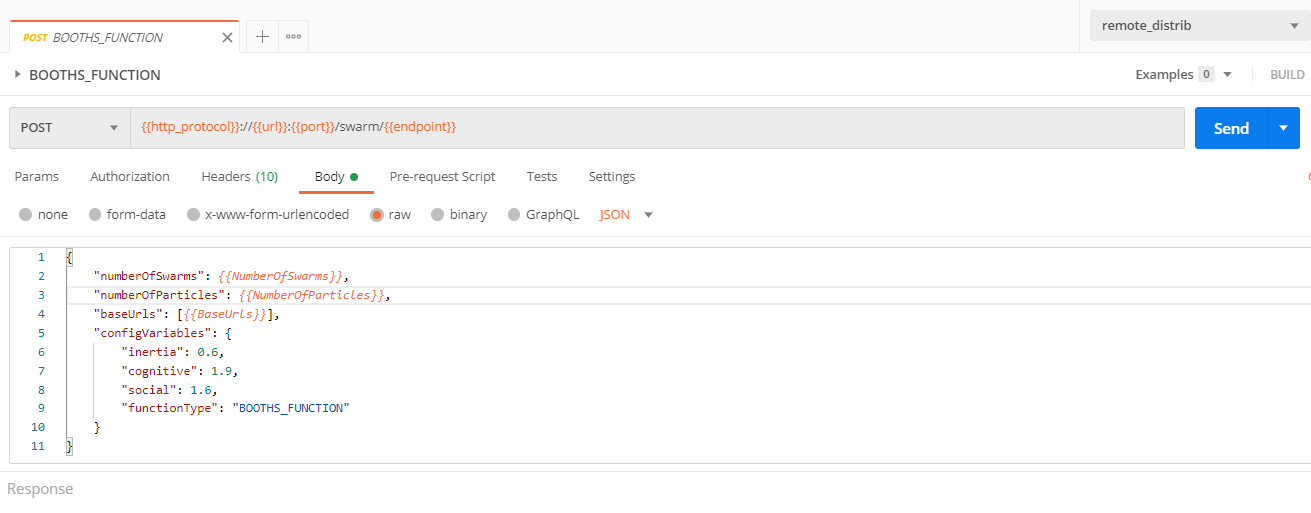
\includegraphics[scale=0.5]{Images/PostmanTest.png}
    \caption{Postman Test}
    \label{fig:PostmanTest}
\end{figure}
In order to accomplish that goal postman was chosen to create the tests with, and newman was used as the test runner. Postman is a "scalable API testing tool that quickly integrates into CI/CD pipelines."\footnote{\url{https://www.guru99.com/postman-tutorial.html}}. Postman allows you to easily define a test for a remote API HTTP endpoint, specifying headers, body parameters etc, and display the response from that API. Postman comes equipped with plenty of development tools, for example it supports environment selection and parameters, allowing developers to substitute values based on the environment they have chosen. Figure \ref{fig:PostmanTest} shows an image of a postman test opened in the Postman application. In the figure it can be seen how the URL can be parameterised using the curly brackets operators \verb|{{Parameter_Name}}|, which can also be applied to body variables.  Postman can organise a series of tests into what it call a test collection, which can be exported to json files and saved locally. 


Newman is the command line implementation of postman. Newman can take these JSON test collection and run them in a batch format. Newman runs on NodeJs, and is installed through NPM. NodeJs is a "an asynchronous event-driven JavaScript runtime, Node.js is designed to build scalable network applications." \footnote{\url{https://nodejs.org/en/about/}}. NPM(Node package manager) is a command line package manager tool that allows developers to download and install javascript libraries to their local development environment. While newman is mainly described as a CLI tool, it has a full API available for developers to use through node. Utilising this API allows for developers to create programs utilising postman test suites, while being able to programatically change parameters as required. 

\subsection{Implementation}
The test harness was split into two main methods for looping, one for the centralised run, and one for the distributed run, however they only differ in one aspect. When adding additional swarms the distributed implementation builds up a list of IP address corresponding to the swarm nodes. The centralised implementation only adds adds the required number swarms to the request. Listing \ref{listing:TestHarness} shows how this loop functions. This is specifically the centralised method, however the distributed method is nearly identical except for some minor configuration changes. The harness first iterates through each fitness function i.e. Beale, Booths and Easom function. For each fitness function test set, the number of swarms is gradually increased from two to ten, and the total number of particles across all swarms in each test increases from 100,000 to 1,000,000. So for example when the test is for two swarms, each swarm will increase from 50,000 particles to 100,000, to 150,000 etc. until the total number of particles is 1,000,000. Each of these tests will keep the same configuration values, and will be run three times so that an average across results may be obtained. The harness is configured to wait for each request to return a response object before moving onto the next request, to avoid overloading the droplets. Newman by default runs asynchronously, so the harness was configured to check every second if a file with the expected test name was written to the disk, and if it has move on, if not keep looping. 

\begin{lstlisting}[basicstyle=\footnotesize, language=JavaScript]
async function centralisedRun() {
    for(var functionId = 0; functionId<= functionNames.length-1; functionId ++) {
        for (var swarmNumber = 1; swarmNumber <= maxNumberSwarms; swarmNumber++) {
            particleIncrement = 1000;
            for (var particleNumber = particleStartNumber; particleNumber <= maxNumberParticles; particleNumber += particleIncrement) {
                runNewmanCode("NON_DISTRIB", functionNames[functionId], "Remote", swarmNumber, particleNumber, baseUrlStringsNonDistributed, nonDistribEndpoint);
                var moveOntoNextTest = false;
                while (!moveOntoNextTest) {
                    moveOntoNextTest = checkIfFilesExist("NON_DISTRIB", functionNames[functionId], swarmNumber, particleNumber);
                    await new Promise(resolve => setTimeout(resolve, 1000));
                }
            }
        }
    }
}
\end{lstlisting}
\captionof{lstlisting}{Test Harness Main Loop}\label{listing:TestHarness}

Listing \ref{listing:NewmanImplShort} shows the newman node implementation code. The implementation allows for a lot of reuse, by accepting parameters for changing the PSO implementation type, number of swarms/particles and fitness function type. The code uses the function name to load up the correct postman collection type, there's only one test in each collection. Utilising the newman API, and correctly loading up the test collection and environment variables file, the method calls out to the remote domain controller and records the responses. Errors are gracefully handled through newmans inbuilt error handling system. This is repeated until all tests have been run across all fitness functions. 

\begin{lstlisting}[basicstyle=\footnotesize, language=JavaScript]
function runNewmanCode(envName, testCollectionName, environmentName, numberOfSwarms, numberOfParticles, baseUrlsSting, endpoint) {
    newman.run({
        collection: require('./Requests/' + testCollectionName + '.postman_collection.json'),
        environment: require('./EnvVariables/' + environmentName + '.postman_environment.json'),
        reporters: 'cli',
        globalVar: [{ "key":"NumberOfSwarms", "value":numberOfSwarms }, {"key":"endpoint", "value": endpoint}, { "key":"NumberOfParticles", "value": numberOfParticles}, { "key":"BaseUrls", "value": baseUrlsSting}]
    }).on('request', function (error, args) {
            fs.writeFile( dir + testCollectionName + "_" + numberOfSwarms + "_" + numberOfParticles + '.result.json', args.response.stream, function (error)
        }
    });
}
\end{lstlisting}
\captionof{lstlisting}{Newman Implementation Code}\label{listing:NewmanImplShort}

Once the method receives a response back from the service, it will use the function name, number of particles/swarms to write out the response to a file with those parameters. Those para maters will be used in its name, allowing each response to be uniquely named, and avoiding overwriting the output file with each new response. 

\section{Data aggregator implementation}
As mentioned in chapter three, multiple test iterations will be run to get averages from the results. In this experiment each function was tested three times for the two implementation types, with swarms increasing from one to ten, and particles in all swarms increasing from one thousand to one hundred thousand. In order to aggregate all the results a simple data aggregation tool was created. The data aggregator needed to load data from each of these three tests runs, get an average value for the following values; Number of iterations, Time to solution and final group best. 

NodeJs was used to load the data and generate the average values, and the system writes the result out as a CSV(Comma separated value) file. Listing \ref{listing:DataAggregationShort} shows the code extract for this. In the listing we can see there is a set header string that will always be outputted at the beginning of the program, this is simply for ease of reading when the CSV is imported into excel. The program iterates through each function, swarm and particle number, and loads the JSON output file. Once it loads the result file for all three test runs, for both implementations it calculates the centralised averages and creates an output string in the CSV format. Once the centralised output string has been generated the program generates the same output string for the distributed implementation. The output string is built up for the same fitness function tests, and then outputted to the file system. 

\begin{lstlisting}[basicstyle=\footnotesize, language=JavaScript]
var outputString = "SWARM_NUMBER,PARTICLE_NUMBER,CENTRALISED_ITERATIONS,CENTRALISED_TIME_TO_SOLUTION,CENTRALISED_FINAL_GROUP_BEST,DISTRIBUTED_ITERATIONS,DISTRIBUTED_TIME_TO_SOLUTION,DISTRIBUTED_FINAL_GROUP_BEST\n";

for (var swarmNumber = 1; swarmNumber <= numberOfSwarms; swarmNumber++) {
    for (var particleNumber = 1000; particleNumber <= maxNumberParticles; particleNumber += particleIncrement) {
        ....
        let centralised_RUN1 = fs.readFileSync(fileUrlCentralised_RUN1);
        ...
        let centralised_data_RUN1 = JSON.parse(centralised_RUN1);
        ...
        var averageCentralisedTTS = Math.round((centralised_data_RUN1.timeToSolution + centralised_data_RUN2.timeToSolution + centralised_data_RUN3.timeToSolution)/3);
        ...

        outputString = outputString + swarmNumber  + "," + particleNumber + "," + averageCentralisedIterations + "," + averageCentralisedTTS + "," + averageCentralisedGbest + ",";
        .....
}
\end{lstlisting}
\captionof{lstlisting}{Data aggregation Implementation}\label{listing:DataAggregationShort}

\section{Implementation conclusion}
This chapter covered in depth how the PSO code implementations where developed, with a specific focus towards coded examples. Each implementation was discussed in detail, along with how the distributed implementation specifically calls swarm nodes on the network. The test harness and data aggregation tools where also covered in depth, with plenty of code extracts supplied. Test un implementation was discussed in some detail, the next chapter will cover this in more detail along with the results obtained from the tests.





% Results, evaluation and discussion chapter 
% ============================================================= %
\chapter{Results, evaluation and discussion}
\section{Introduction}
This chapter discusses the results obtained from running the experiment described in detail in chapters three and four. Results from the centralised and distributed implementations will be presented and compared. As discussed in chapter three, several fitness functions where tested in this experiment, this chapter will expand on each for both implementations, with a primary focus on the time to solution value. This chapter will also evaluate the results, with some discussion taking place. 

\section{Centralised Testing and Results}
Chapter three and four described the process of running the experiment in detail, in this section the results from those experiment runs will be presented. Each fitness function will be examined and results will be presented. All results are an average of three tests runs in order to compensate for the random element in PSO. Results were compared in a like for like manner, meaning when we compare the number of particles between a two swarm test and a ten swarm test, we are comparing the total number of particles in the test, not how many particles on each swarm. To further expand on that example, when comparing 100,000 particle tests, we look at there being 50,000 particles on each swarm in the two swarm test, and 10,000 particles on each swarm in the 10 swarm tests. This goes for both the centralised and distributed implementation tests. 

\subsection{Easom Function}
The first function to cover is the centralised Easom test runs. Figure \ref{fig:Centralised_TTS_Easom_Results} shows the results when looking at the time to solution(TTS). In the results we can see that as the number of particles increases, the time to solution increases at a disproportionate rate. TTS for each swarm tends to increase at the same rate, except for the ten swarm test runs, where the TTS is slightly longer at the beginning, but increases at a much greater degree closer to the 1,000,000 particles tests.

\begin{figure}[H]
    \centering
    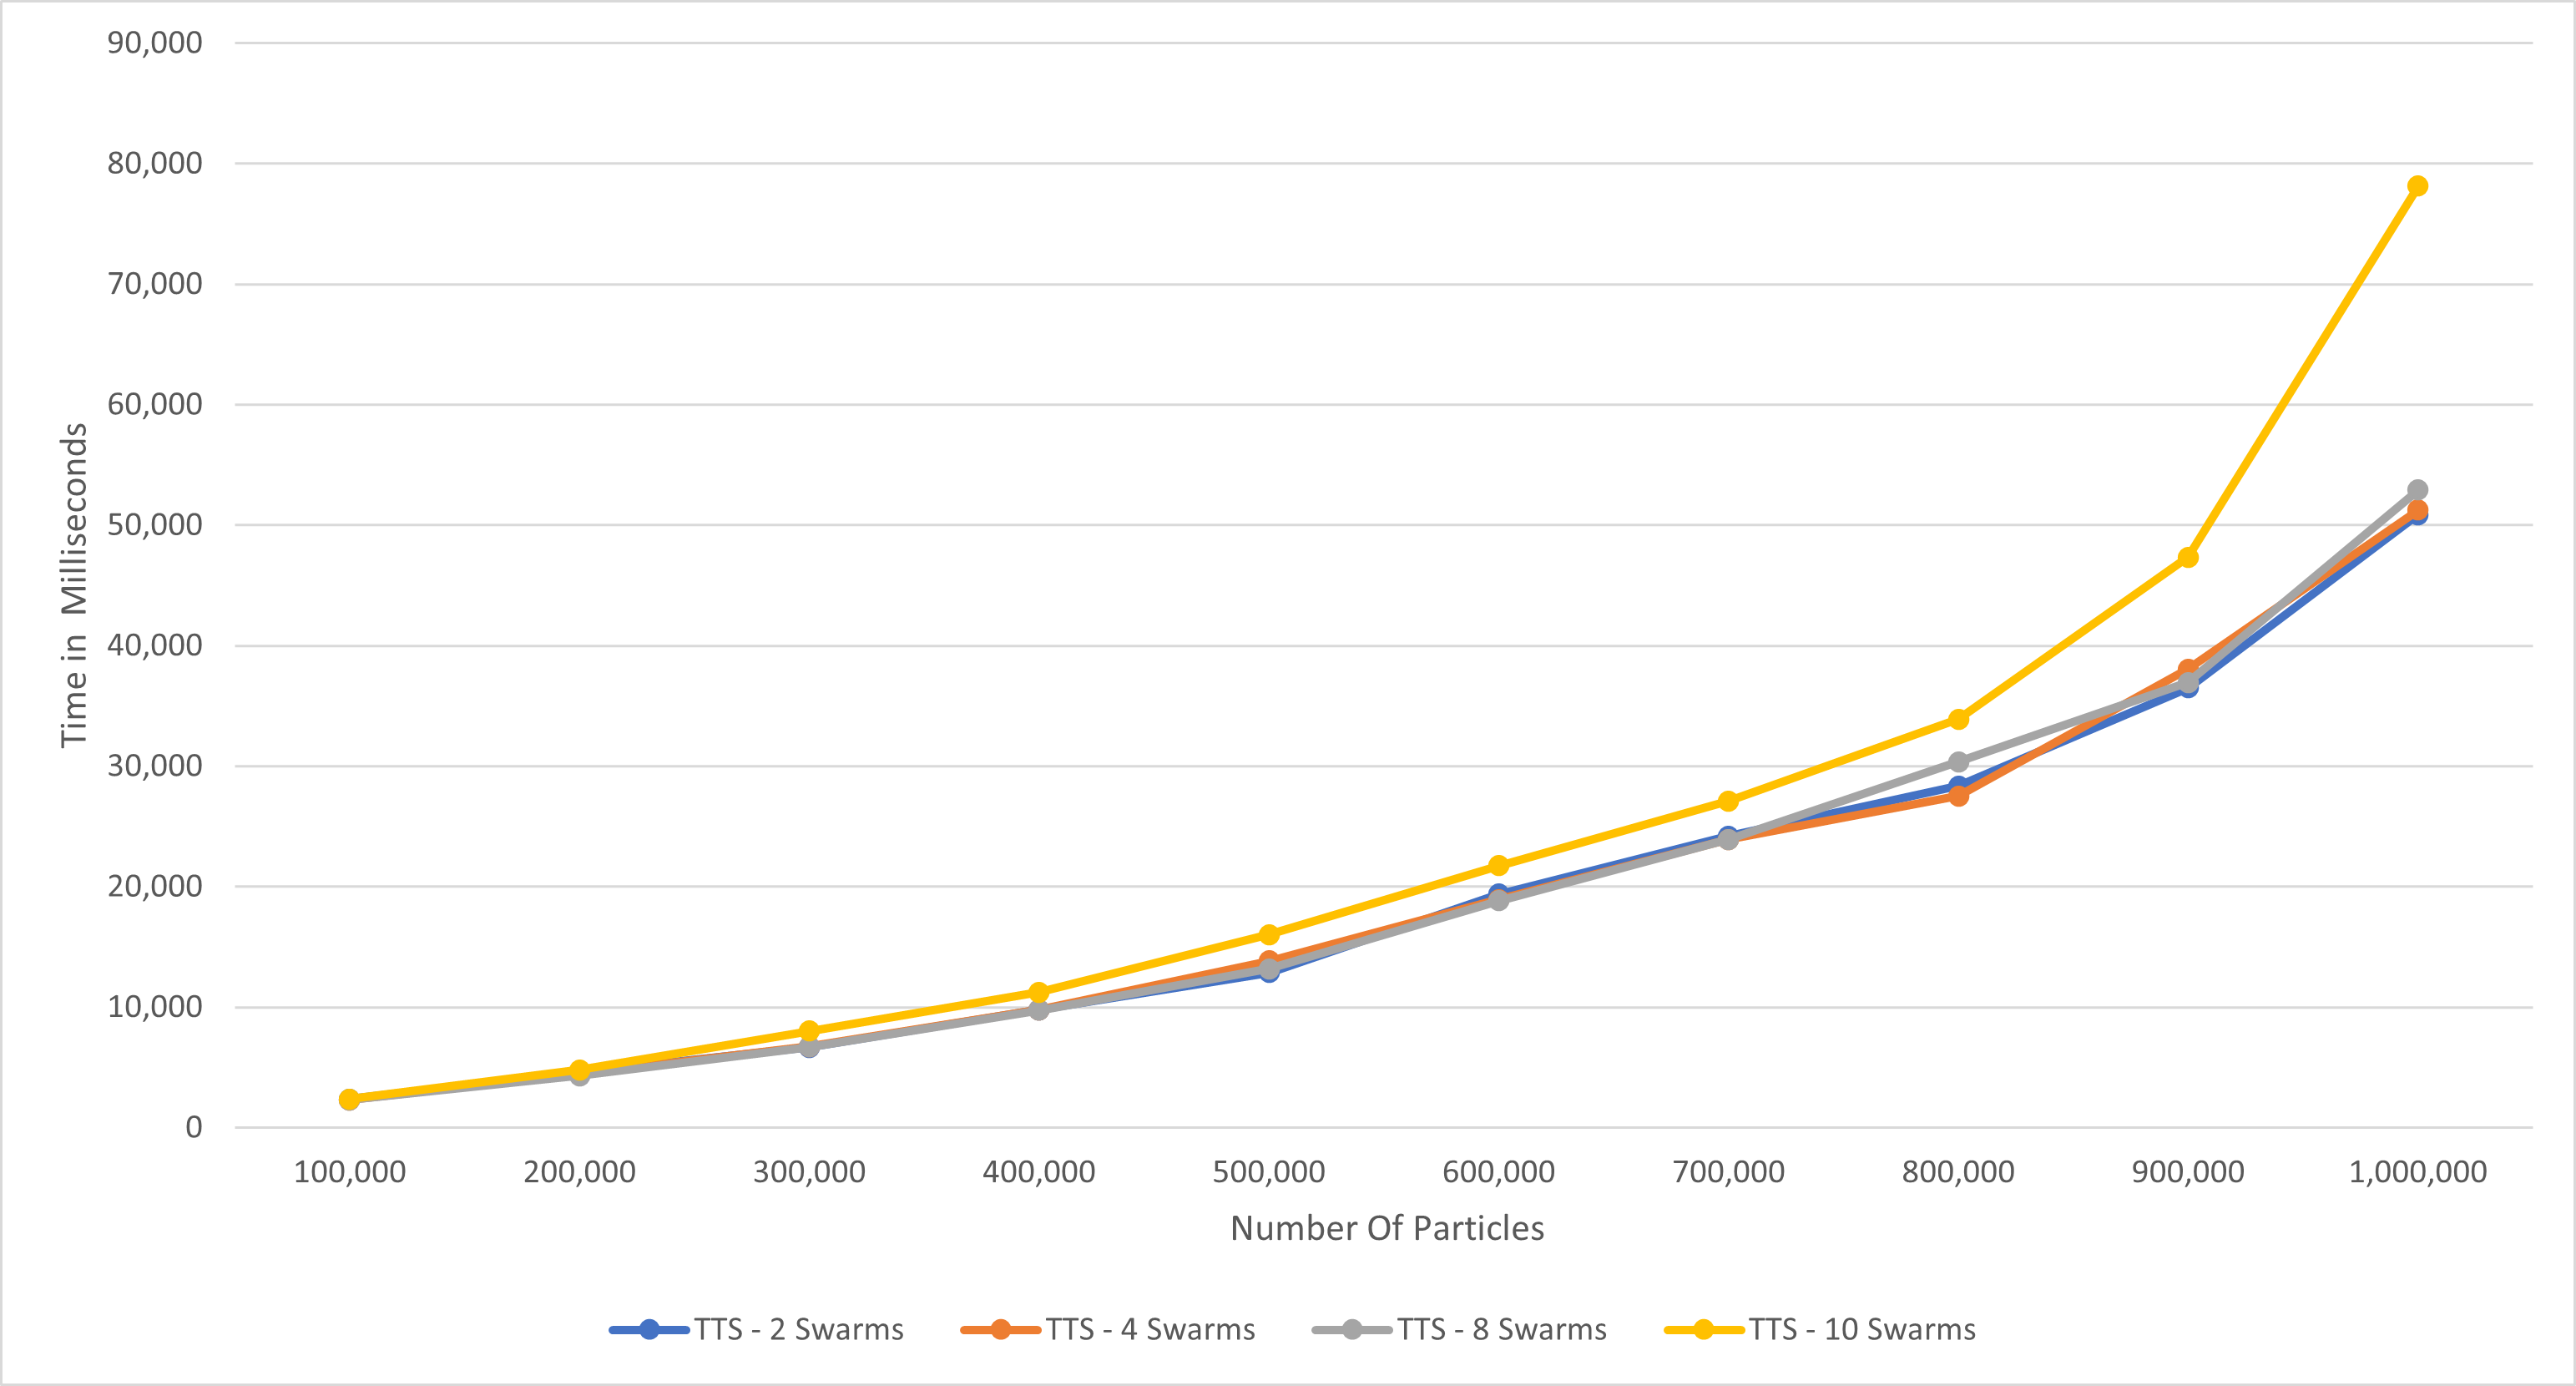
\includegraphics[scale=0.45]{Images/Graphs/CentralisedEasomTTS.png}
    \caption{Centralised TTS Easom Results}
    \label{fig:Centralised_TTS_Easom_Results}
\end{figure}

Figure \ref{fig:Centralised_Epoc_Easom_Results} shows the number of epochs or iterations taken to reach a solution for each of the swarms. All swarms display a downward trend in the number of iterations it takes to reach a solution, with the two and four swarms coming in at the lowest number of iterations at the maximum number of particles, one million particles. From the figure it can be seen that the number of iterations, while on a downward trend, can have a lot of variance as the particles increase in the tests, ie in the two swarm test the average iterations jumps from 114 iterations for 600,000, to 120 iterations for 700,000 particles. As the swarms increase the variance between particles increments decreases. 

\begin{figure}[H]
    \centering
    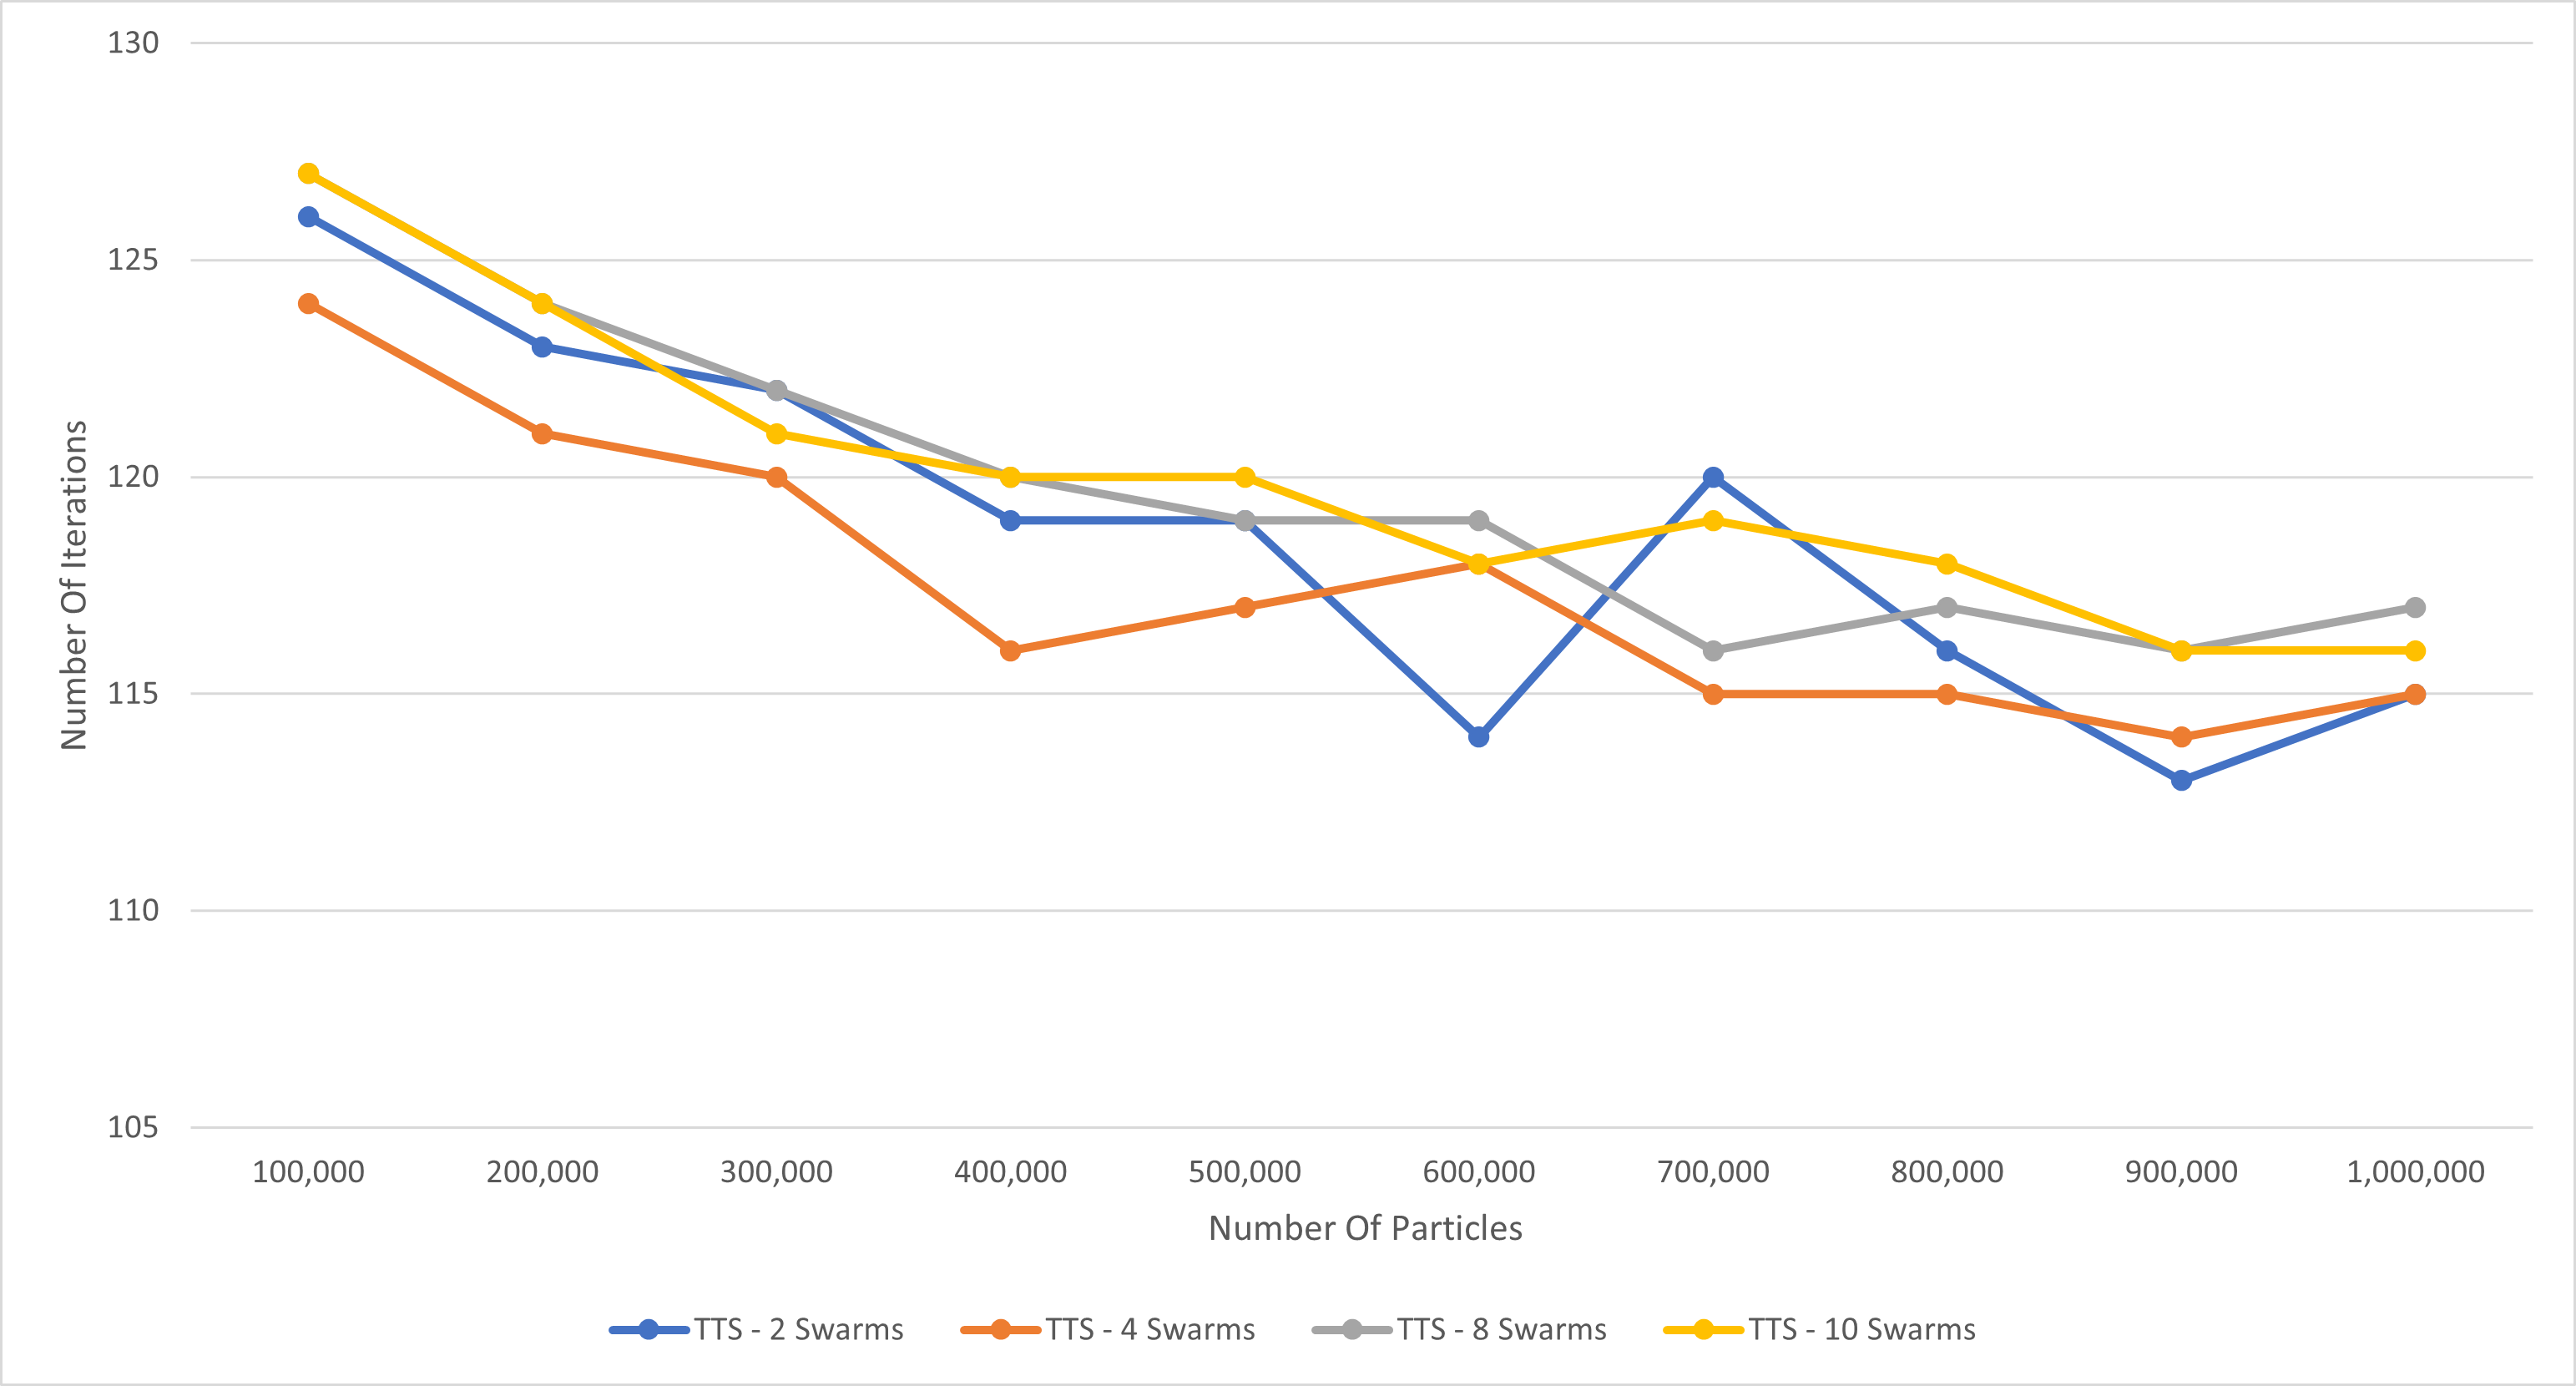
\includegraphics[scale=0.45]{Images/Graphs/CentralisedEasomEpoch.png}
    \caption{Centralised Iterations Easom Results}
    \label{fig:Centralised_Epoc_Easom_Results}
\end{figure}

\subsection{Booths Function}
Looking at the Booths function results in figure \ref{fig:Centralised_TTS_Booths_Results} we see it closely follow the Easom function results, in that the general trend on the results looks to be at an exponential increase. Once again the the test runs where ten swarms are used show a slight increase in the TTS at lower numbers of particles, and a large increase towards the one million particles run.

\begin{figure}[H]
    \centering
    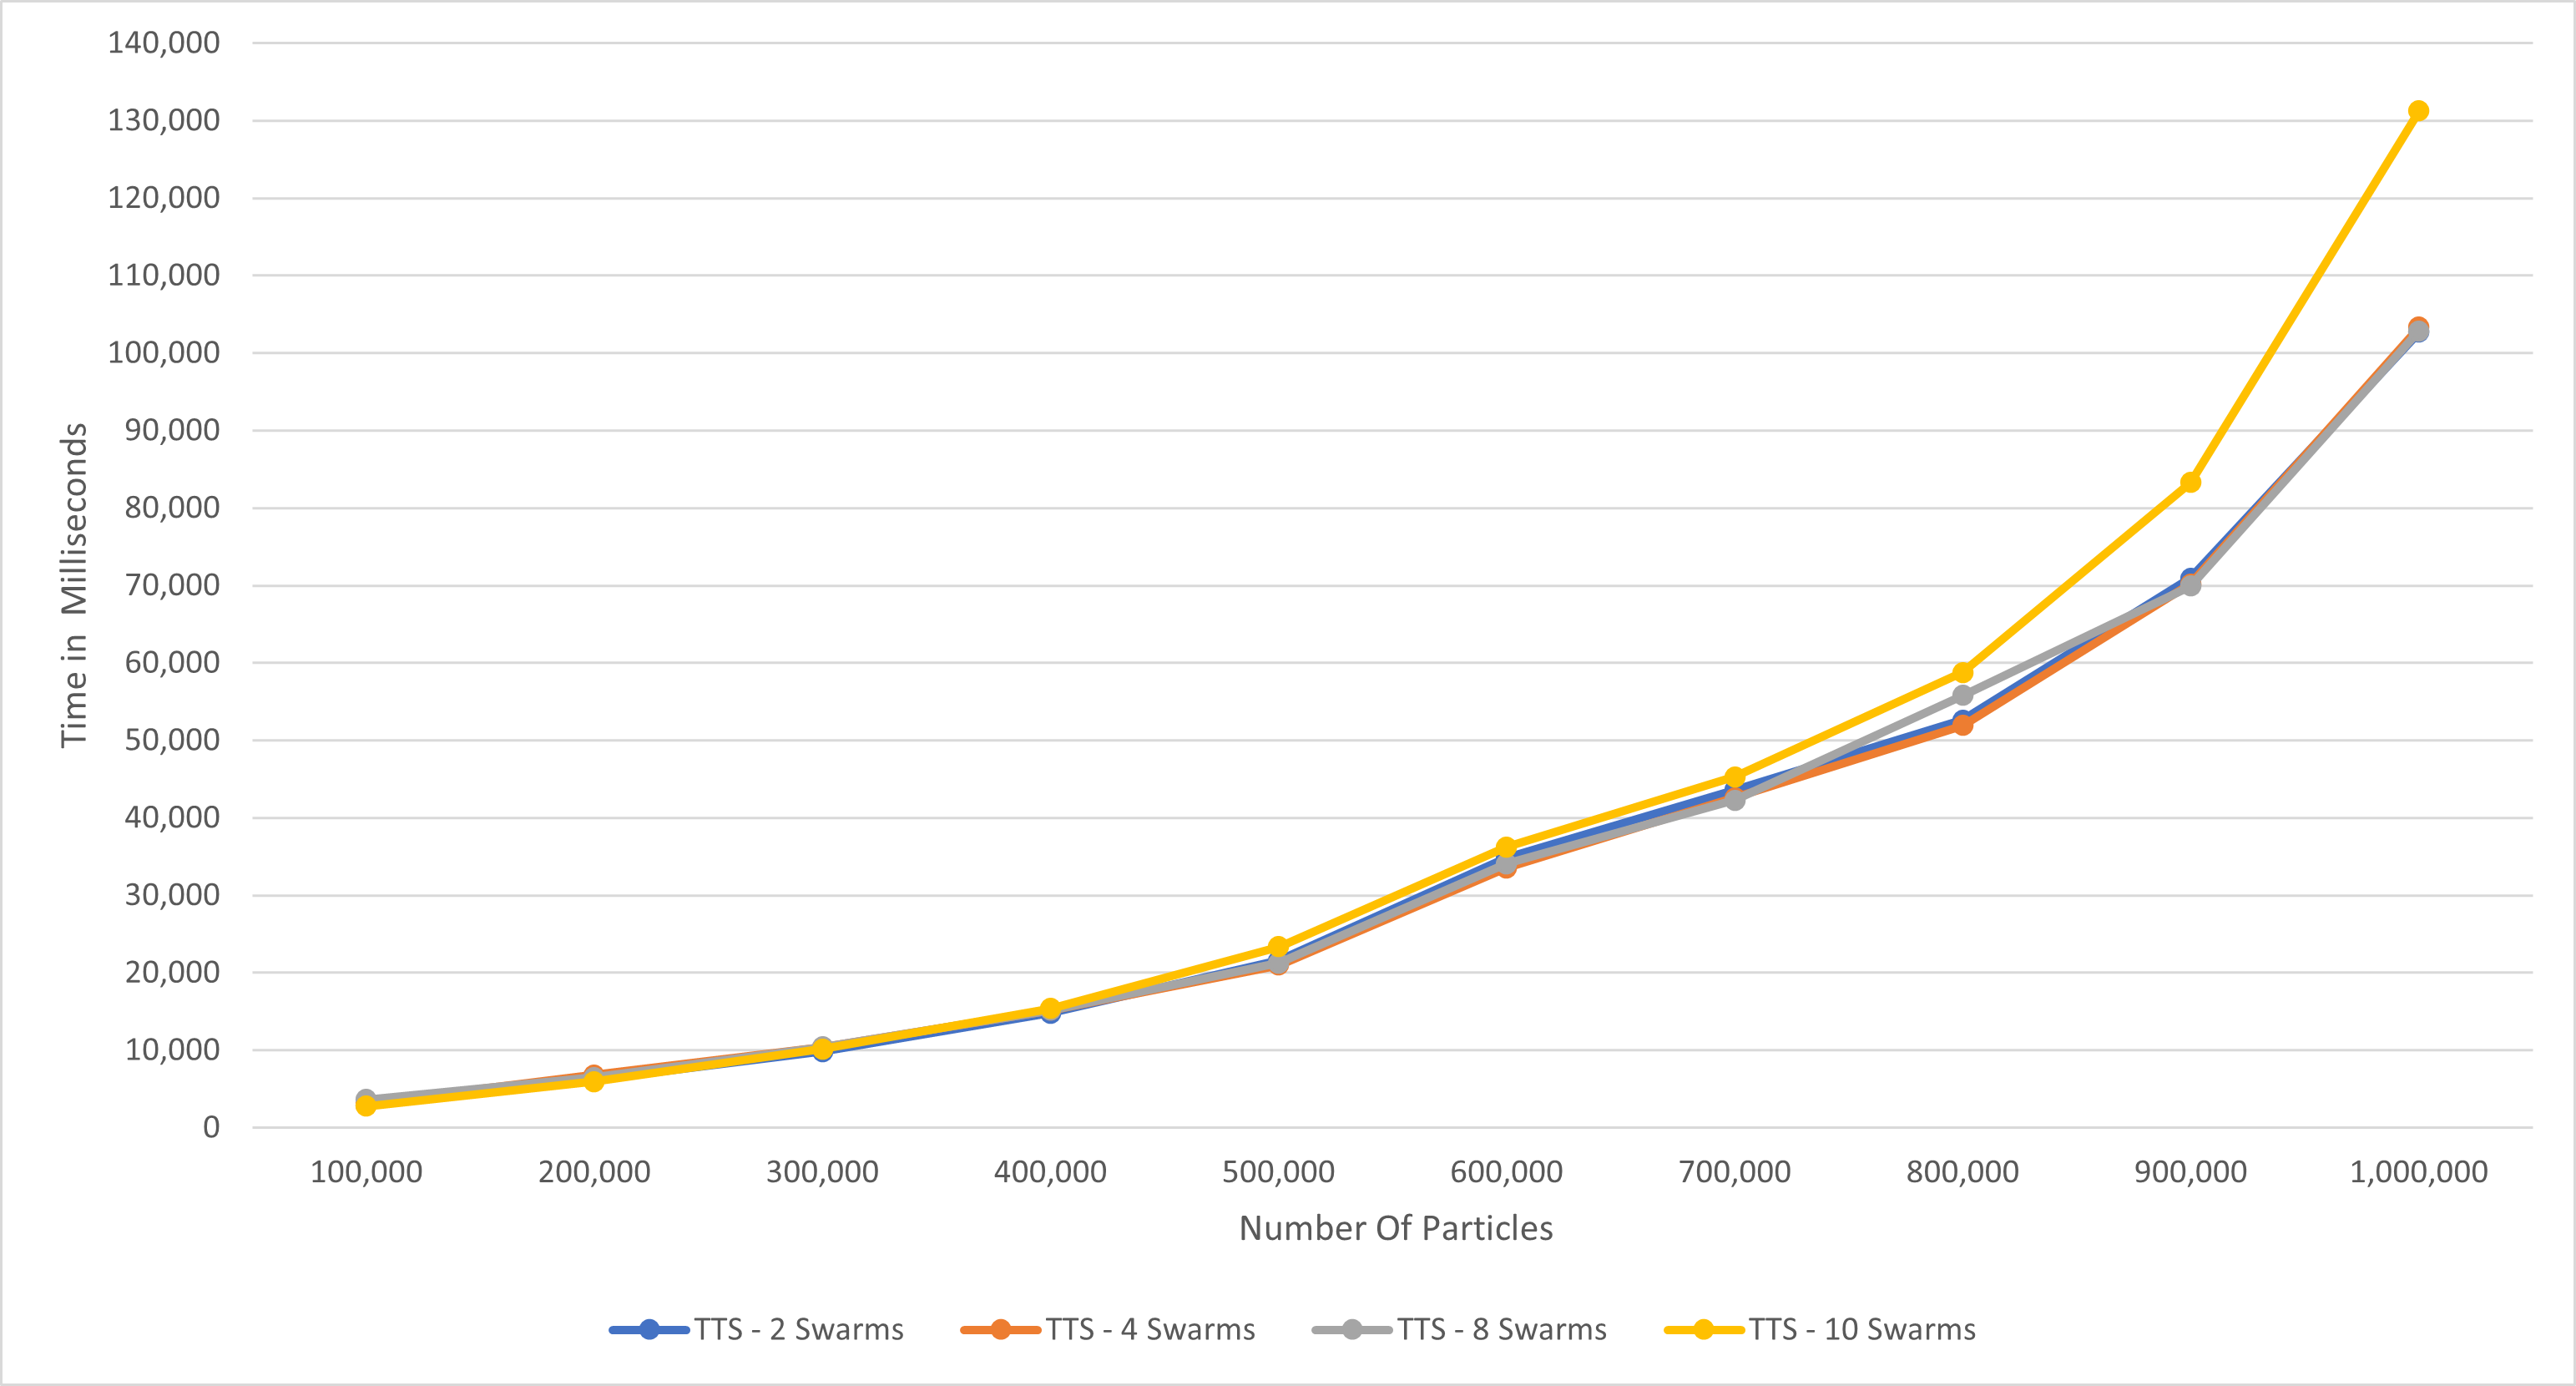
\includegraphics[scale=0.45]{Images/Graphs/CentralisedBoothsTTS.png}
    \caption{Centralised TTS Booths Results}
    \label{fig:Centralised_TTS_Booths_Results}
\end{figure}

Figure \ref{fig:Centralised_Epoc_Booths_Results} shows the results of the average iterations obtained by each swarm in testing. Similar to the Easom results the figure showcases a downward trend in the number of iterations as particles increase. Again the results show that the lower number of swarms, two and fours swarms, obtained a lower number of iterations at the higher number of particles. 

\begin{figure}[H]
    \centering
    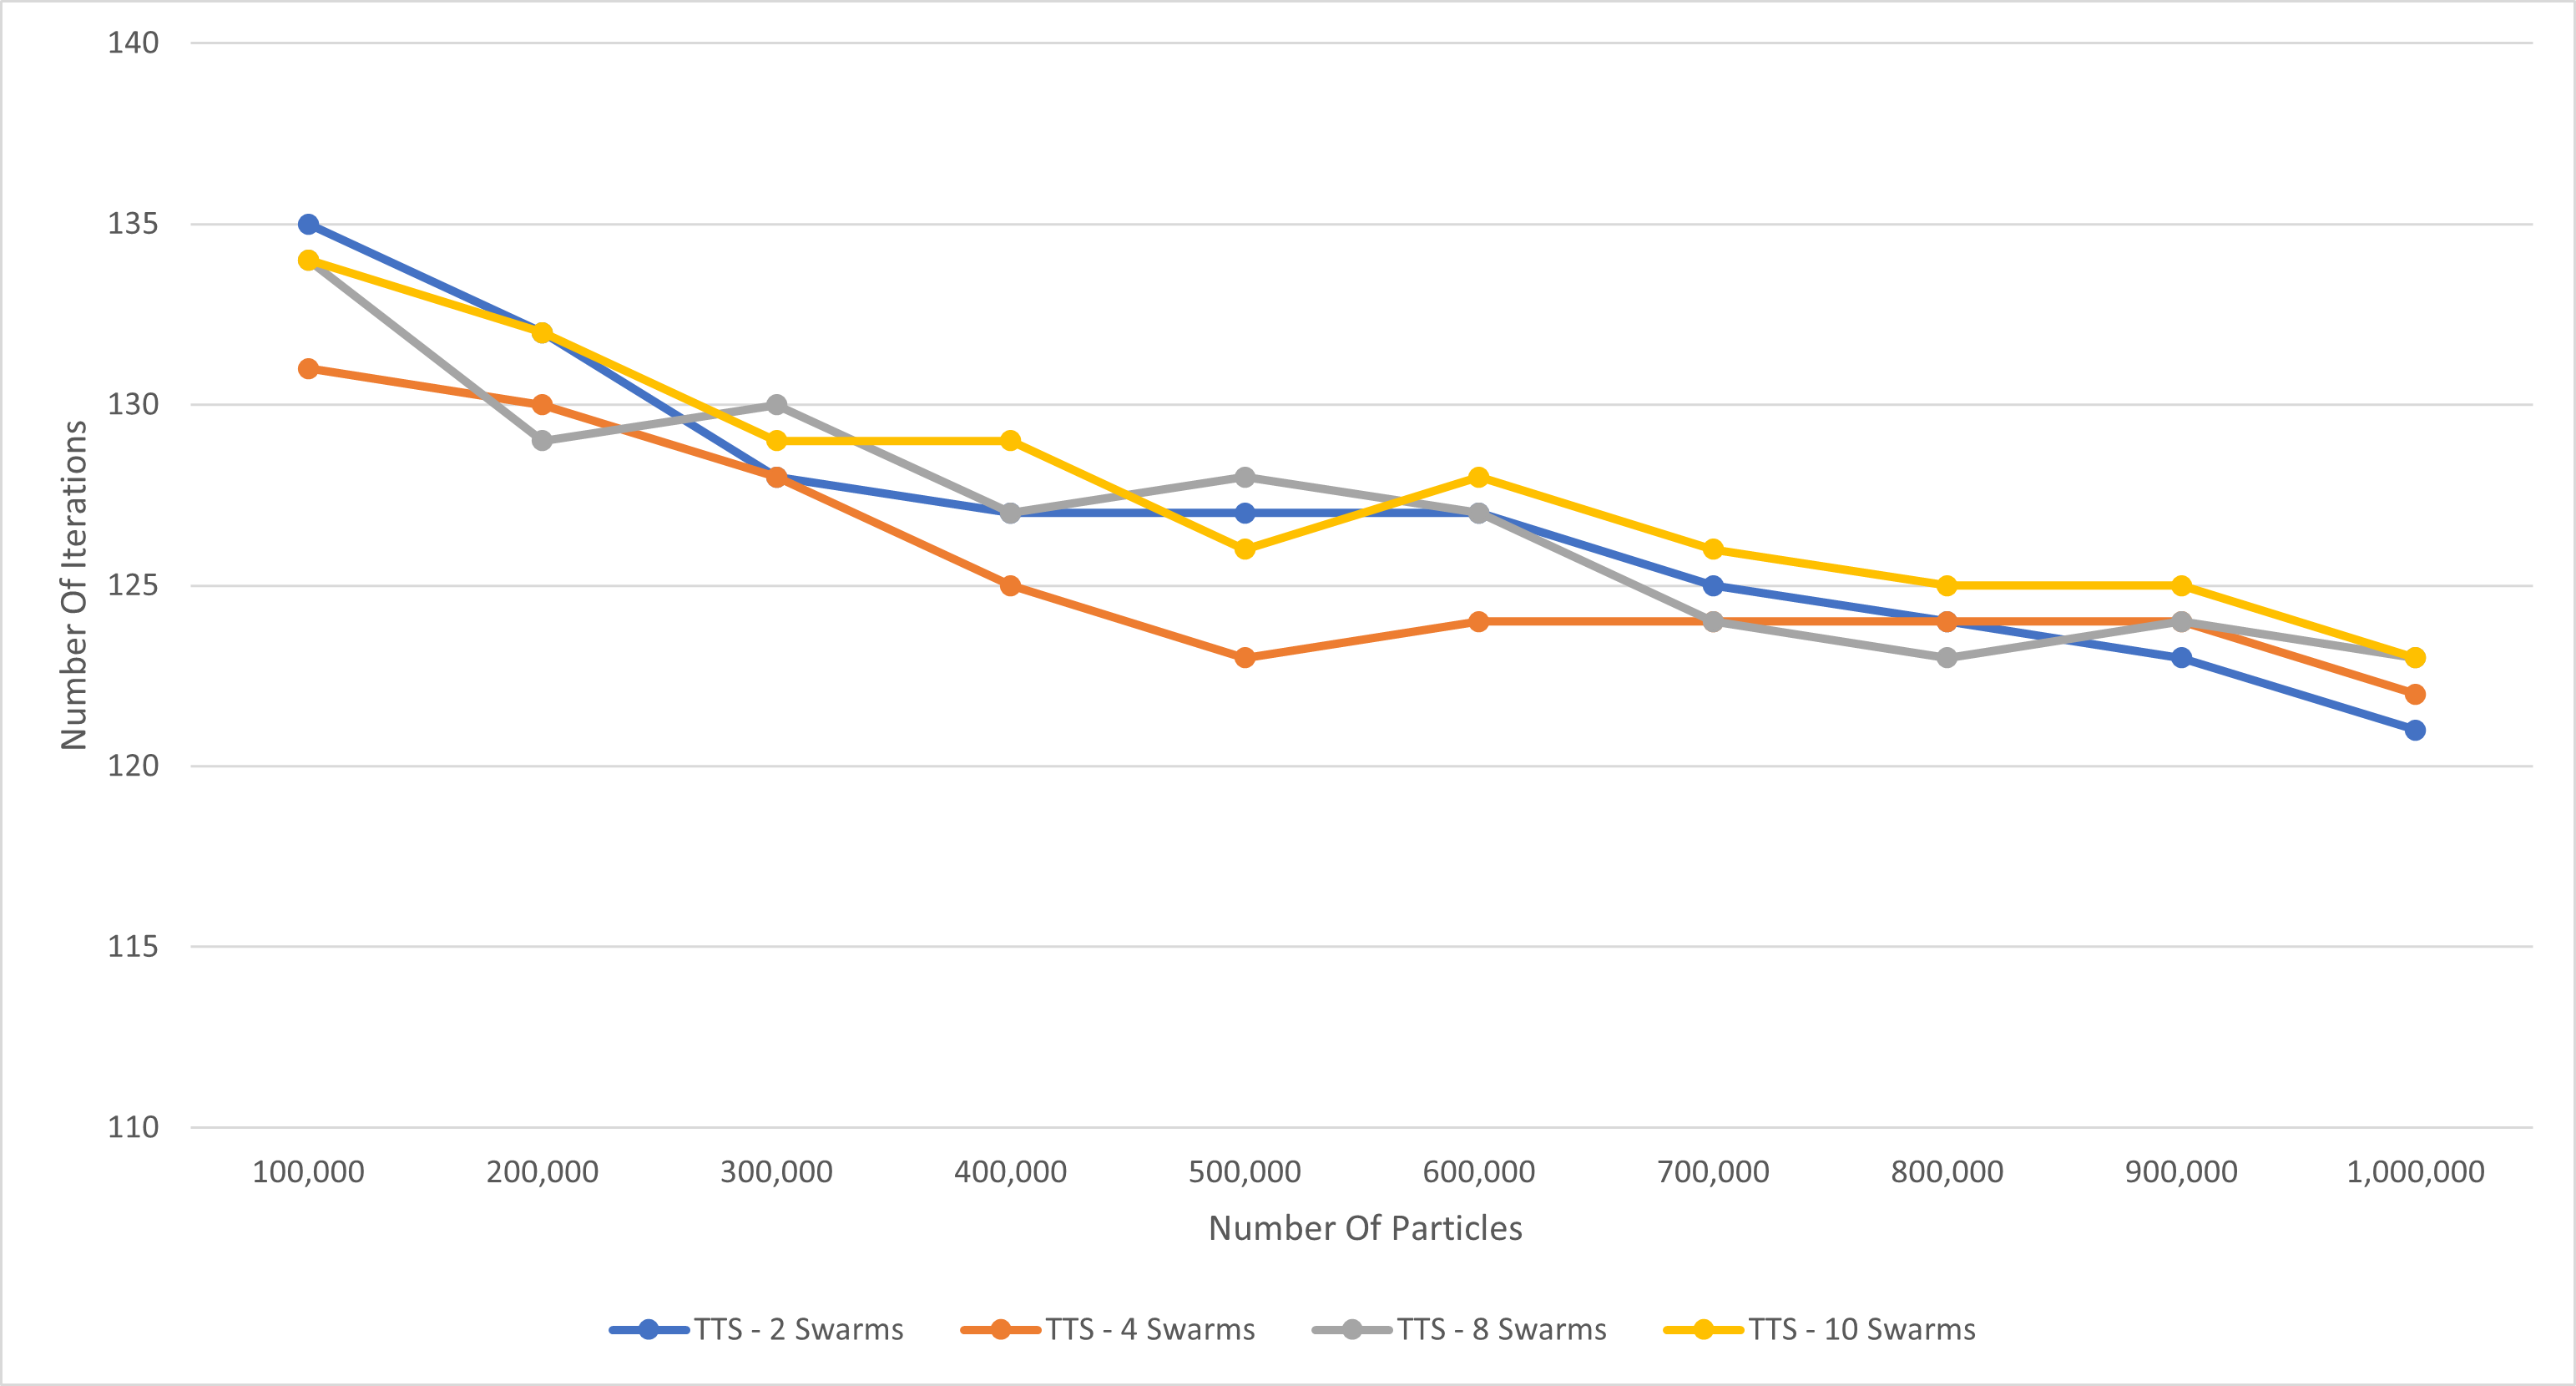
\includegraphics[scale=0.45]{Images/Graphs/CentralisedBoothsEpoch.png}
    \caption{Centralised Iterations Booths Results}
    \label{fig:Centralised_Epoc_Booths_Results}
\end{figure}

\subsection{Beale Function}

Looking at the Beale TTS results in figure \ref{fig:Centralised_TTS_Beale_Results}, the same general trends from Easom and Booths function can be seen, with the general trend looking to be exponential. Again the higher number of swarms tends to end up with a higher TTS as particles increase. 

\begin{figure}[H]
    \centering
    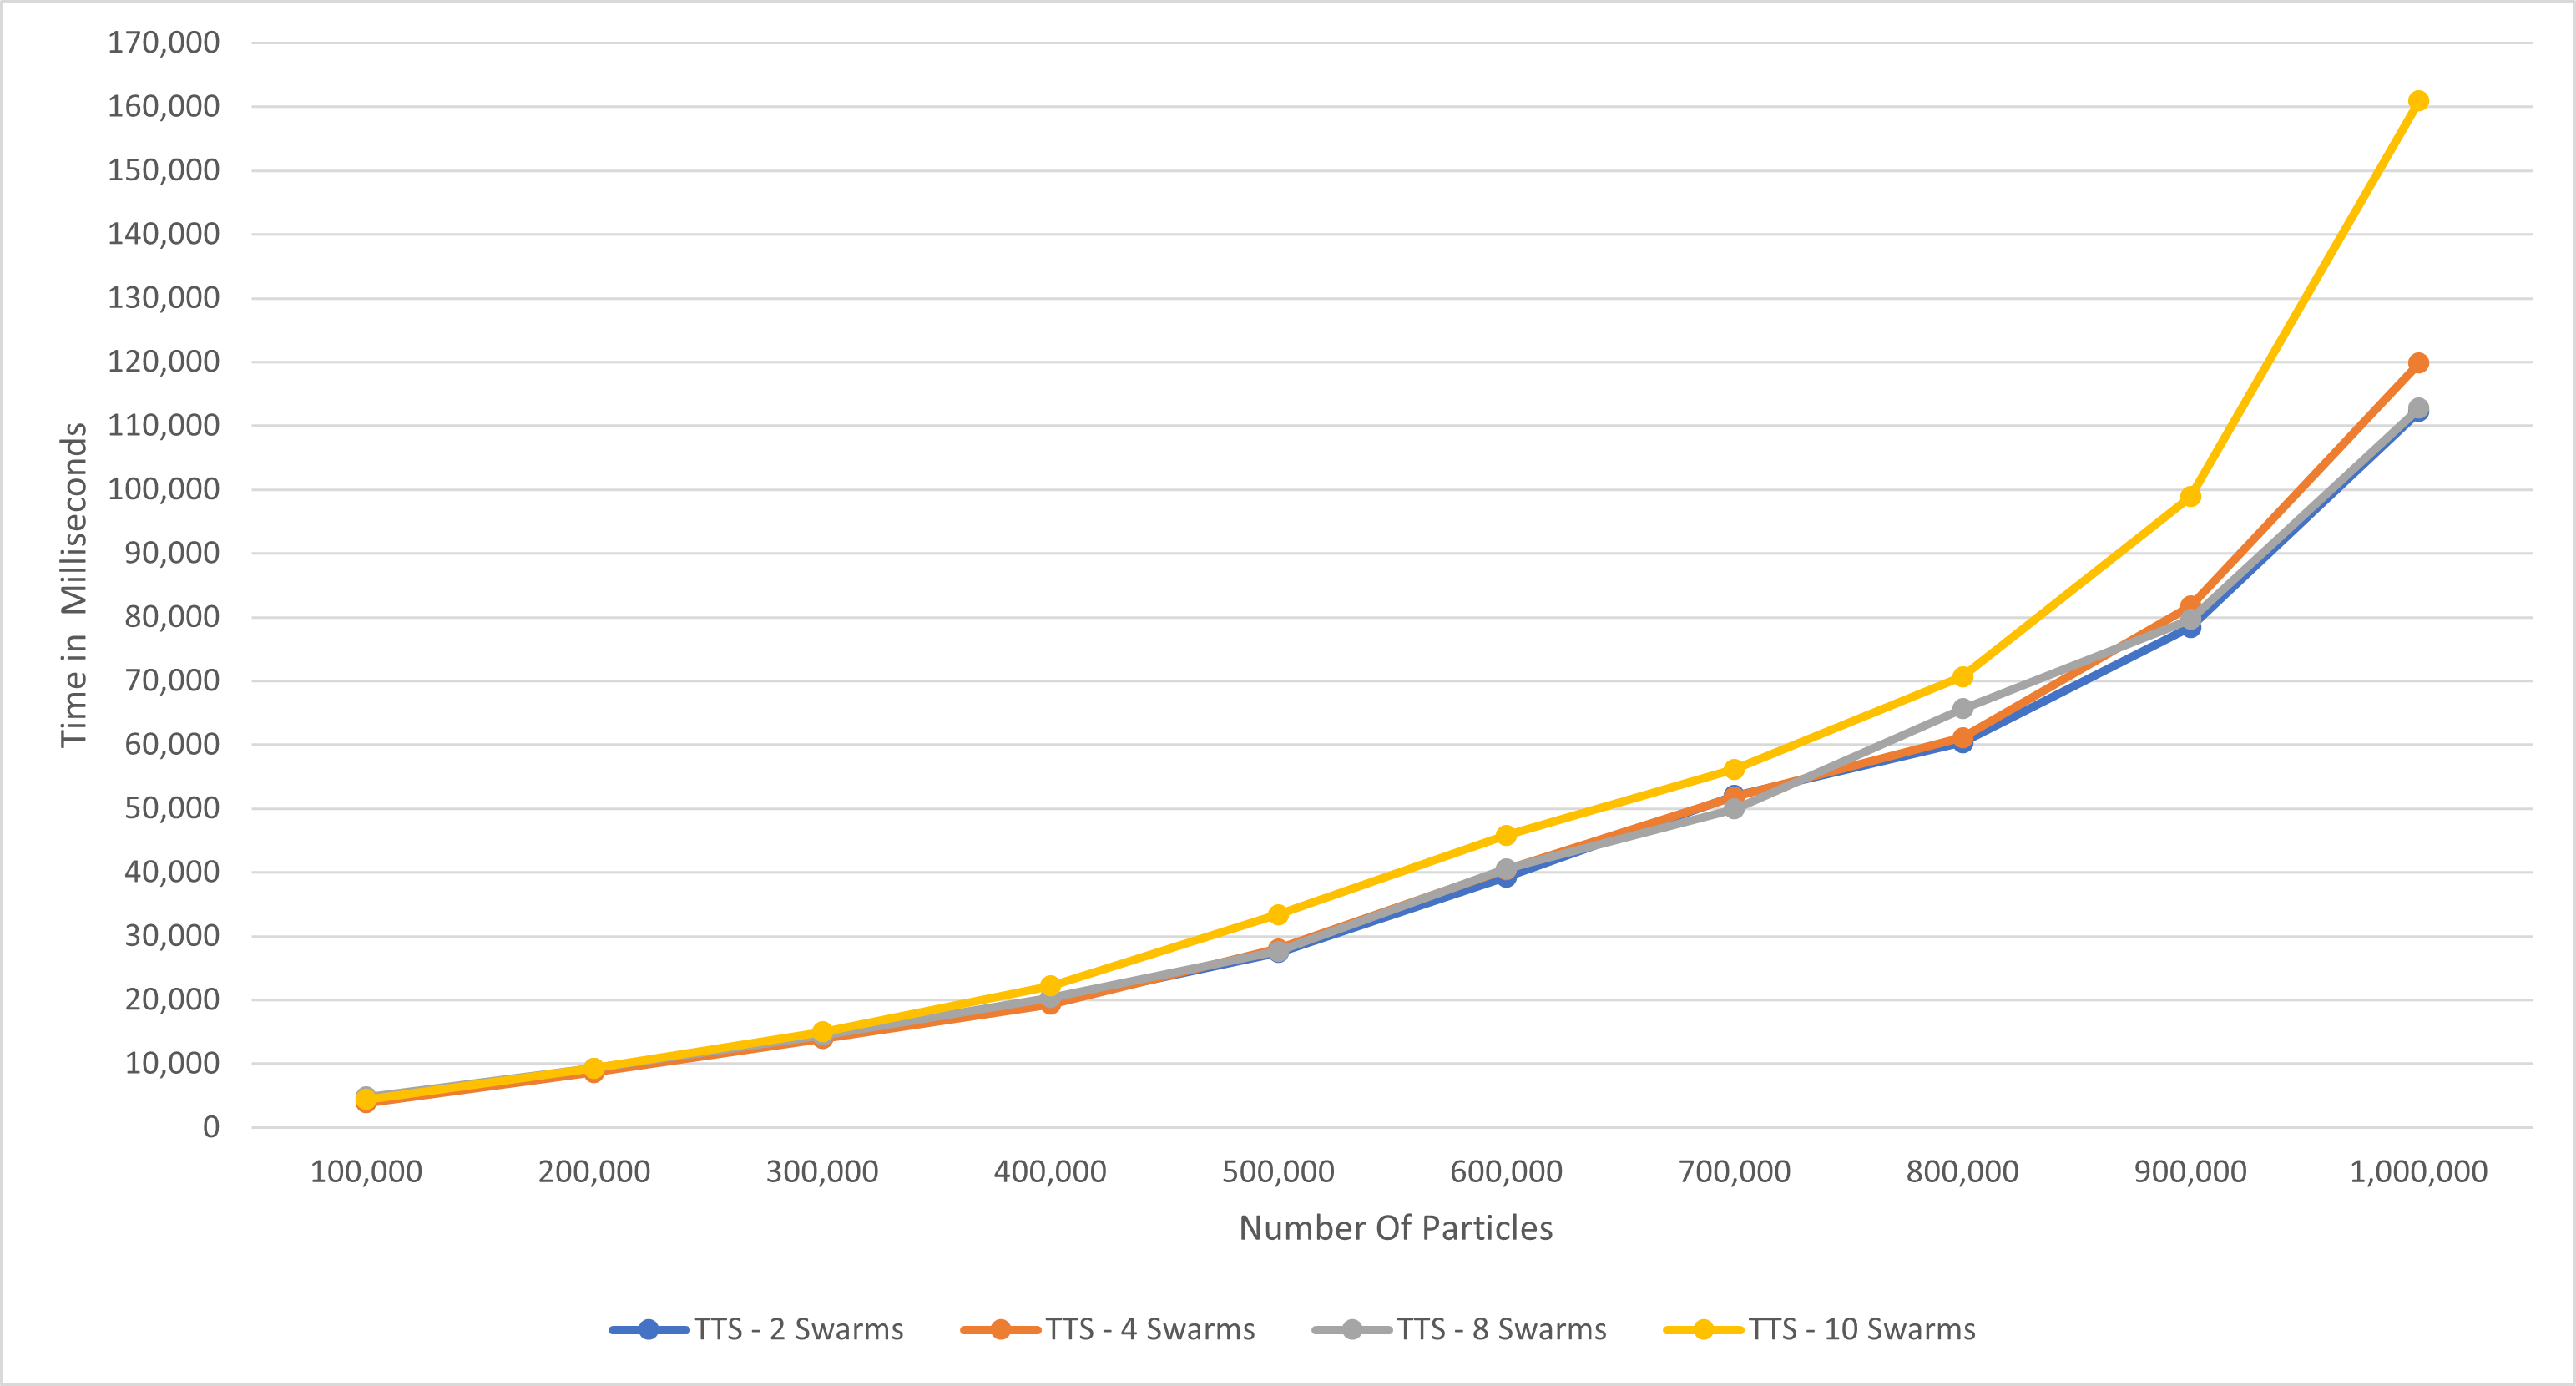
\includegraphics[scale=0.45]{Images/Graphs/CentralisedBealeTTS.png}
    \caption{Centralised TTS Beale Results}
    \label{fig:Centralised_TTS_Beale_Results}
\end{figure}

Figure \ref{fig:Centralised_Epoc_Beale_Results} shows the number of epochs each swarm took to get to a solution. Once again the general trend is that the number of epochs decreases with the increased number of particles, with some variations between the particle increments. Similar to Booths and Beale function the lower number of swarms, two and four swarms had, on average, a lower number of epochs to reach a solution.  

\begin{figure}[H]
    \centering
    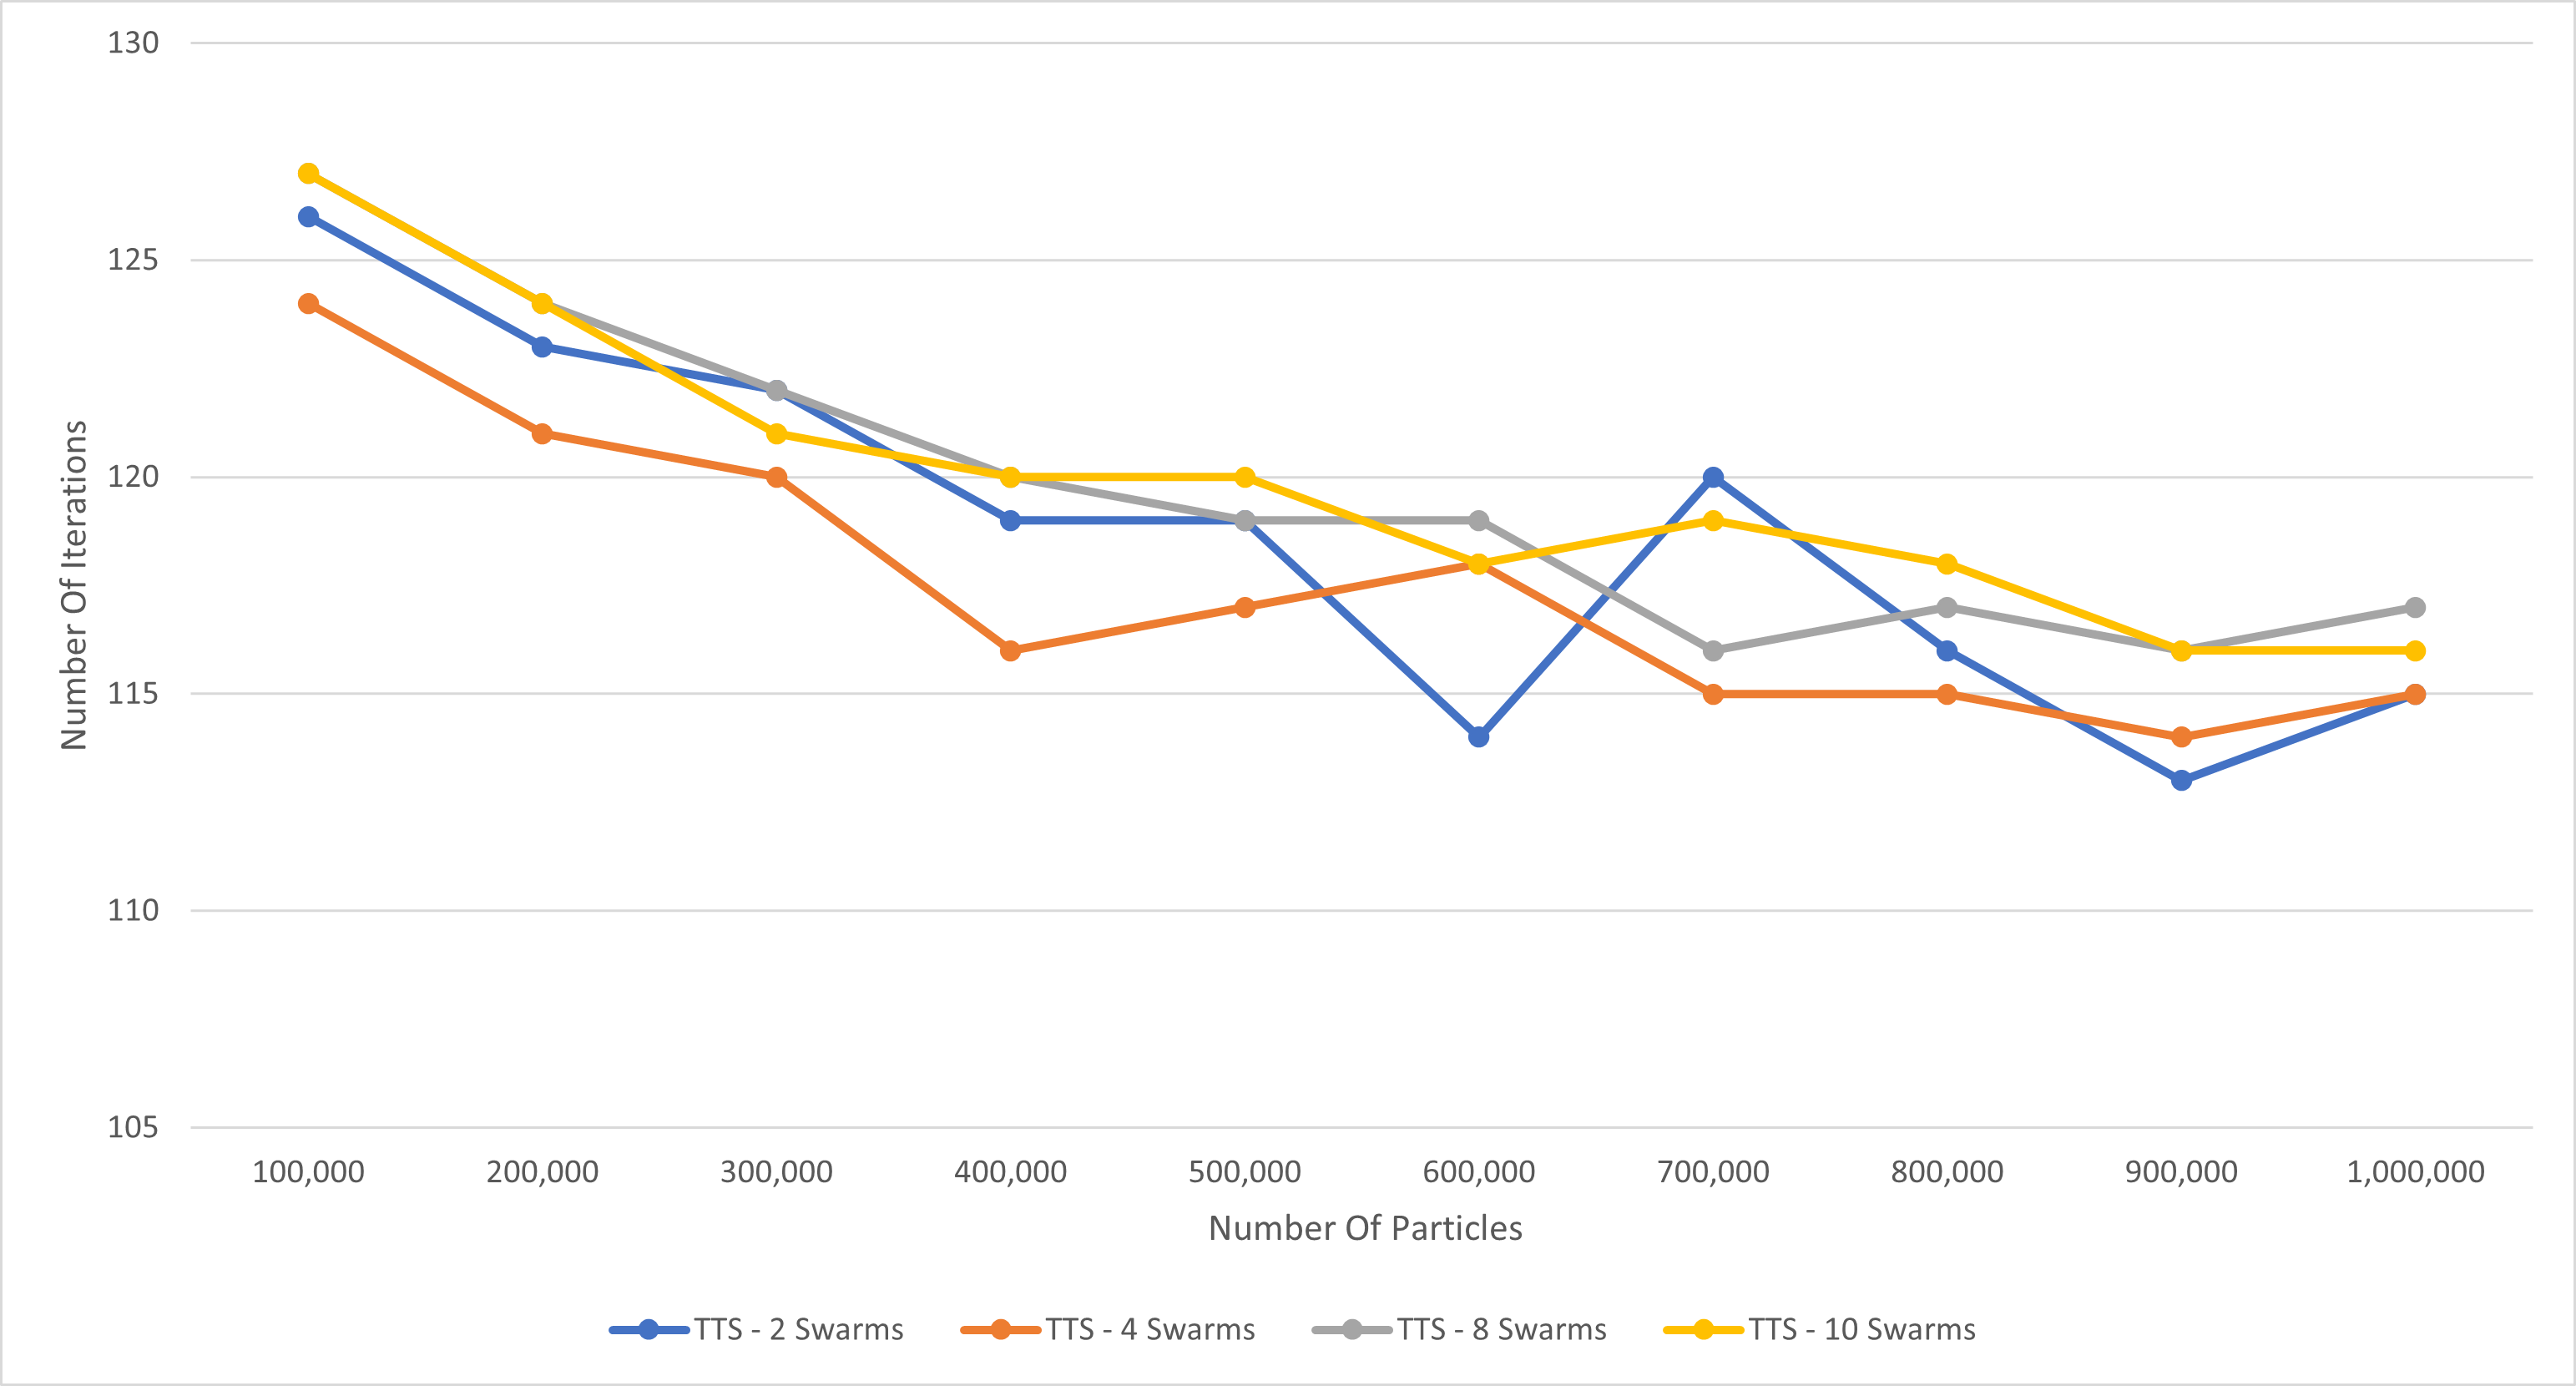
\includegraphics[scale=0.45]{Images/Graphs/CentralisedBealeEpoch.png}
    \caption{Centralised Iterations Beale Results}
    \label{fig:Centralised_Epoc_Beale_Results}
\end{figure}

\section{Distributed results}
This section examines the results from the distributed implementation tests, using the same format as the centralised results section. Each fitness function's results will be presented the, primarily focusing on the TTS and number of Epochs to solution, along with a small amount of commentary on these results. 

\subsection{Easom Function}
Looking at the Easom function first, figure \ref{fig:Distributed_TTS_Easom_Results} shows the TTS results. TTS appears to linearly increase with the number of particles, across all number of swarms. At the upper end of the experiment bounds, with one million particles the two swarm tests appear to increase at a great rate than the four, eight and ten swarm tests, all of which appear to continue the same rate of increase in TTS. There are some variations in this linear increase, most notably the eight swarm tests show a large decrease in TTS at the 800,000 particle point, but otherwise the variations are relatively minor. 

\begin{figure}[H]
    \centering
    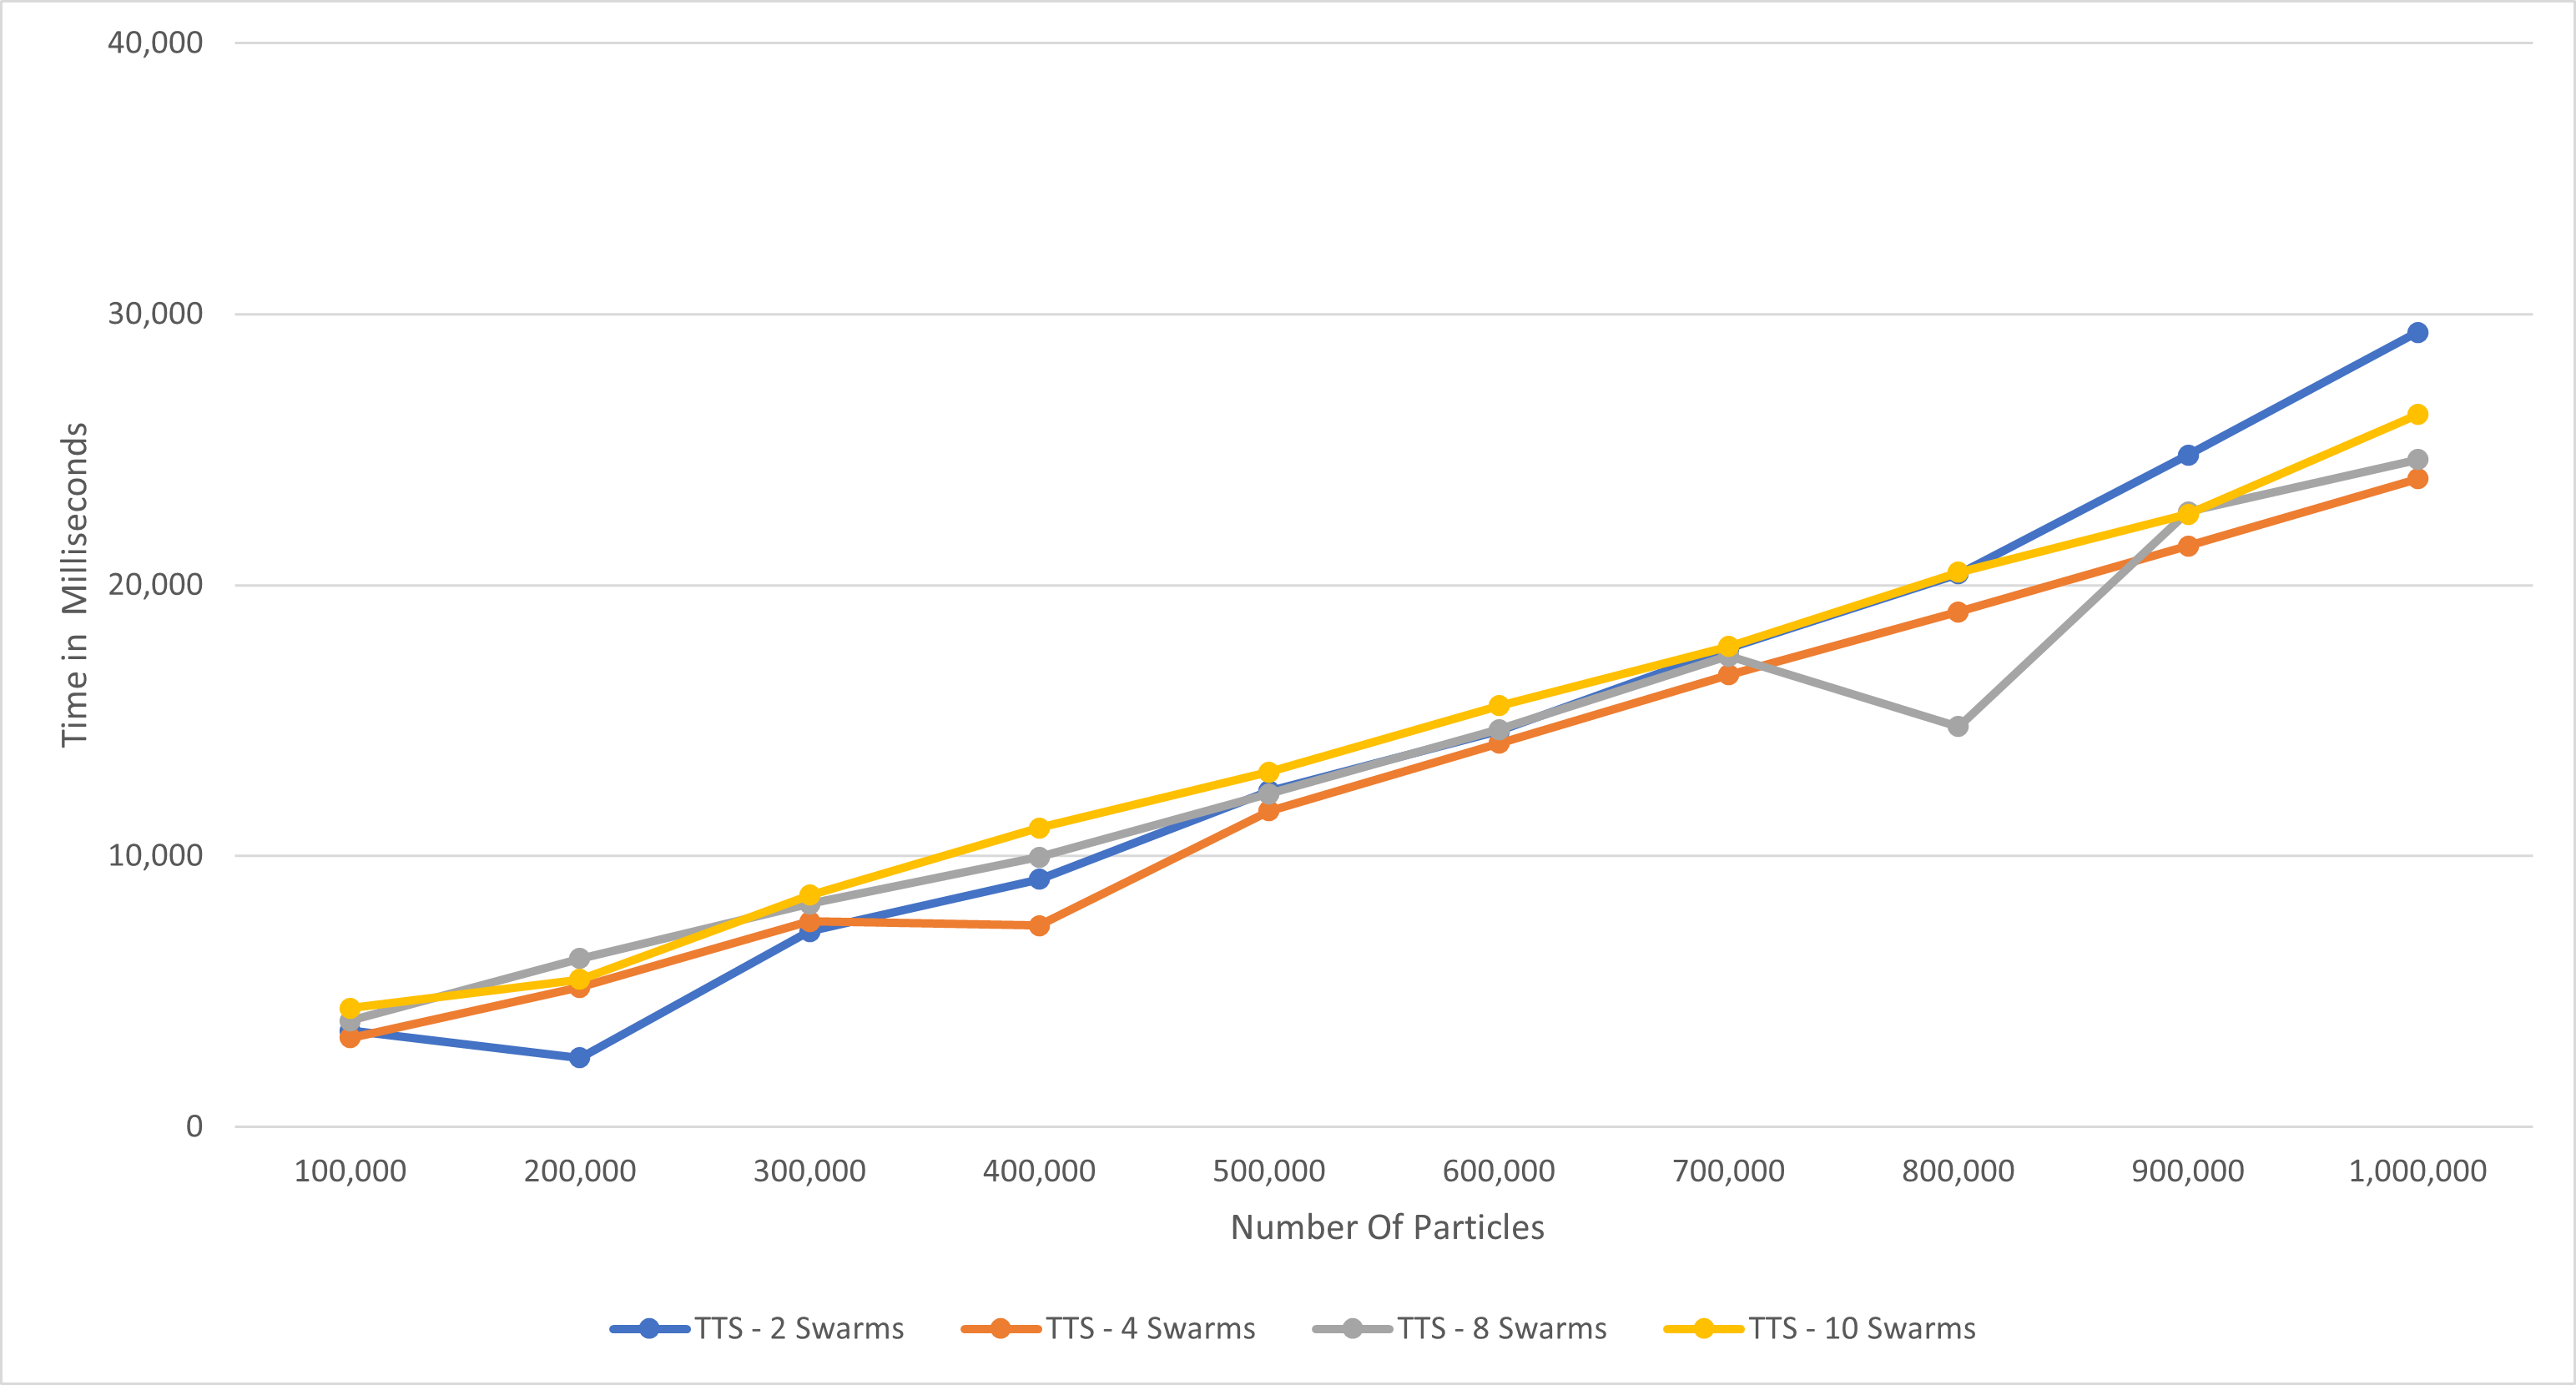
\includegraphics[scale=0.45]{Images/Graphs/DistributedEasomTTS.png}
    \caption{Distributed TTS Easom Results}
    \label{fig:Distributed_TTS_Easom_Results}
\end{figure}

Figure \ref{fig:Distributed_Epoc_Easom_Results} shows the number of epochs to solution results. From that we can see the general trend is a linear decrease, however it is a very slight decrease. The two swarm and ten swarm tests show the least amount of change in results, with the two swarm tests decreasing by two epochs from start to finish, and the ten swarm tests decreasing by three epochs. The eight and four swarm tests showed a greater deal of variance, with the eight and four swarm tests decreasing by nine iterations.

\begin{figure}[H]
    \centering
    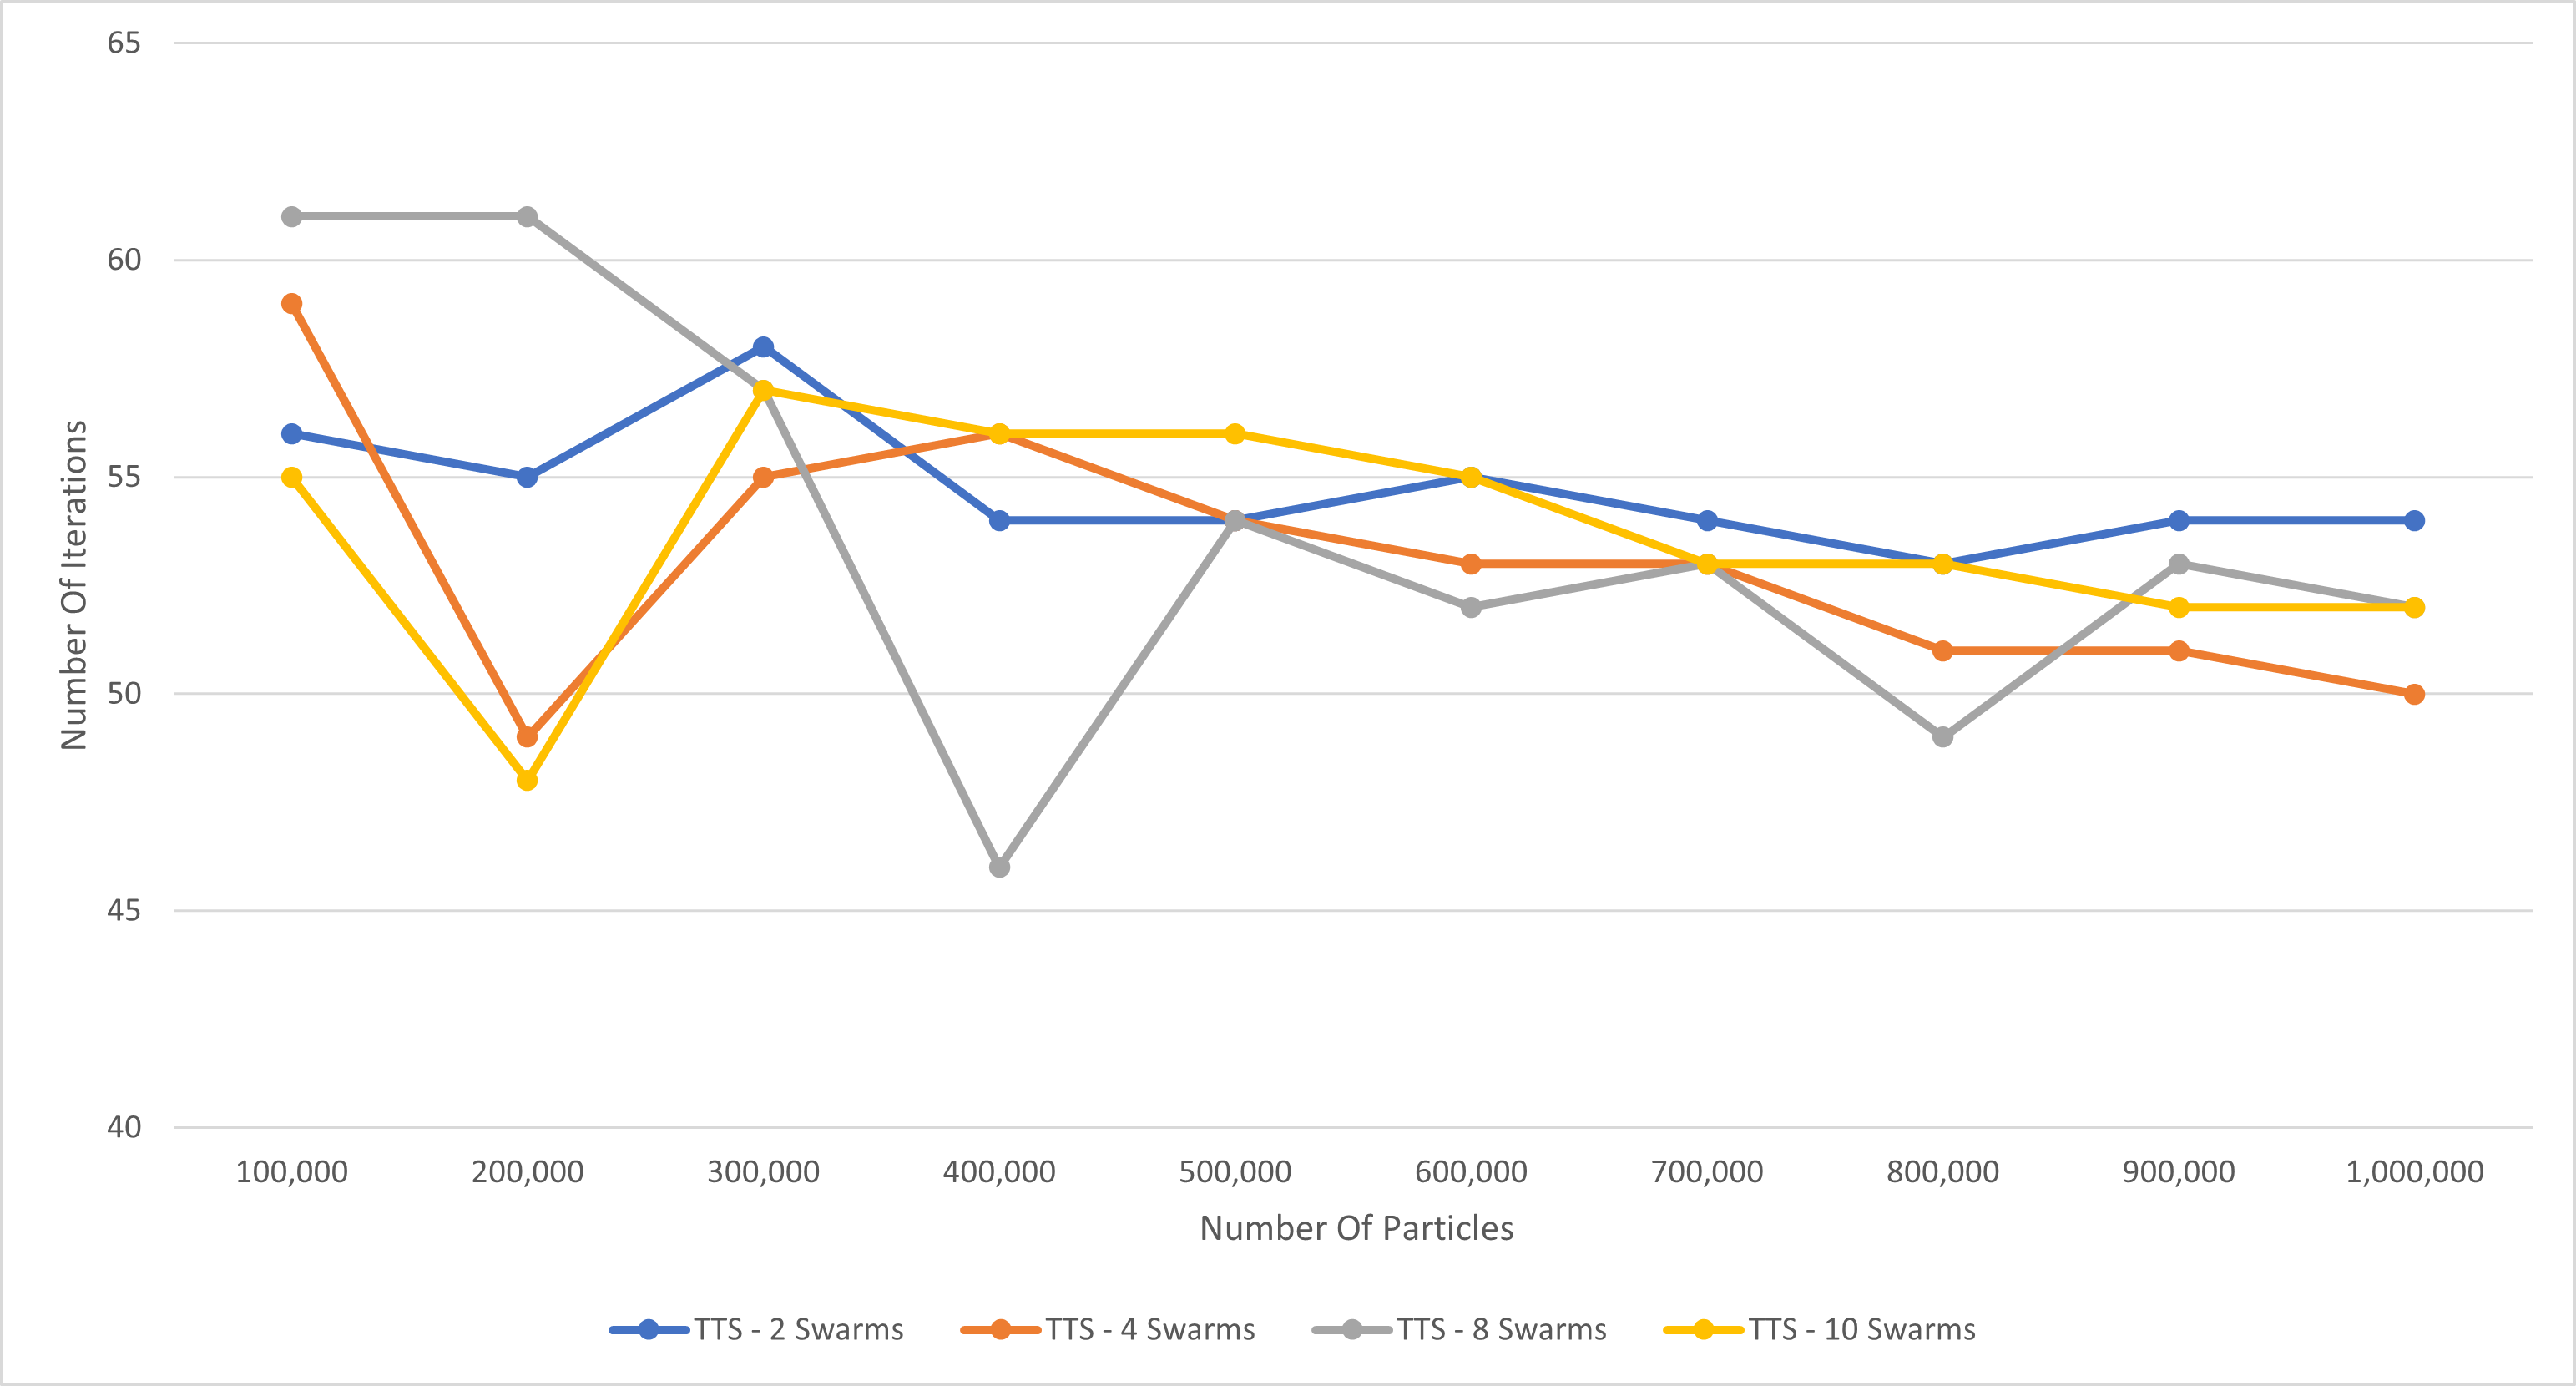
\includegraphics[scale=0.45]{Images/Graphs/DistributedEasomEpoch.png}
    \caption{Distributed Iterations Easom Results}
    \label{fig:Distributed_Epoc_Easom_Results}
\end{figure}

\subsection{Booths Function}
Looking next at booths function figure \ref{fig:Distributed_TTS_Booths_Results} shows the TTS results. Looking at the results shows similar trends as the Easom function results, with the overall trend appearing to be a linear increase in TTS as the number of particles increases. Two swarm tests once again appear to increase at a more aggressive rate towards the upper particle numbers. The ten swarm tests show an overall higher TTS than any other number of swarms. Eight swarm tests showed a large decrease in TTS at the 800,000 particles interval, but resumes the same trend at the next interval. 

\begin{figure}[H]
    \centering
    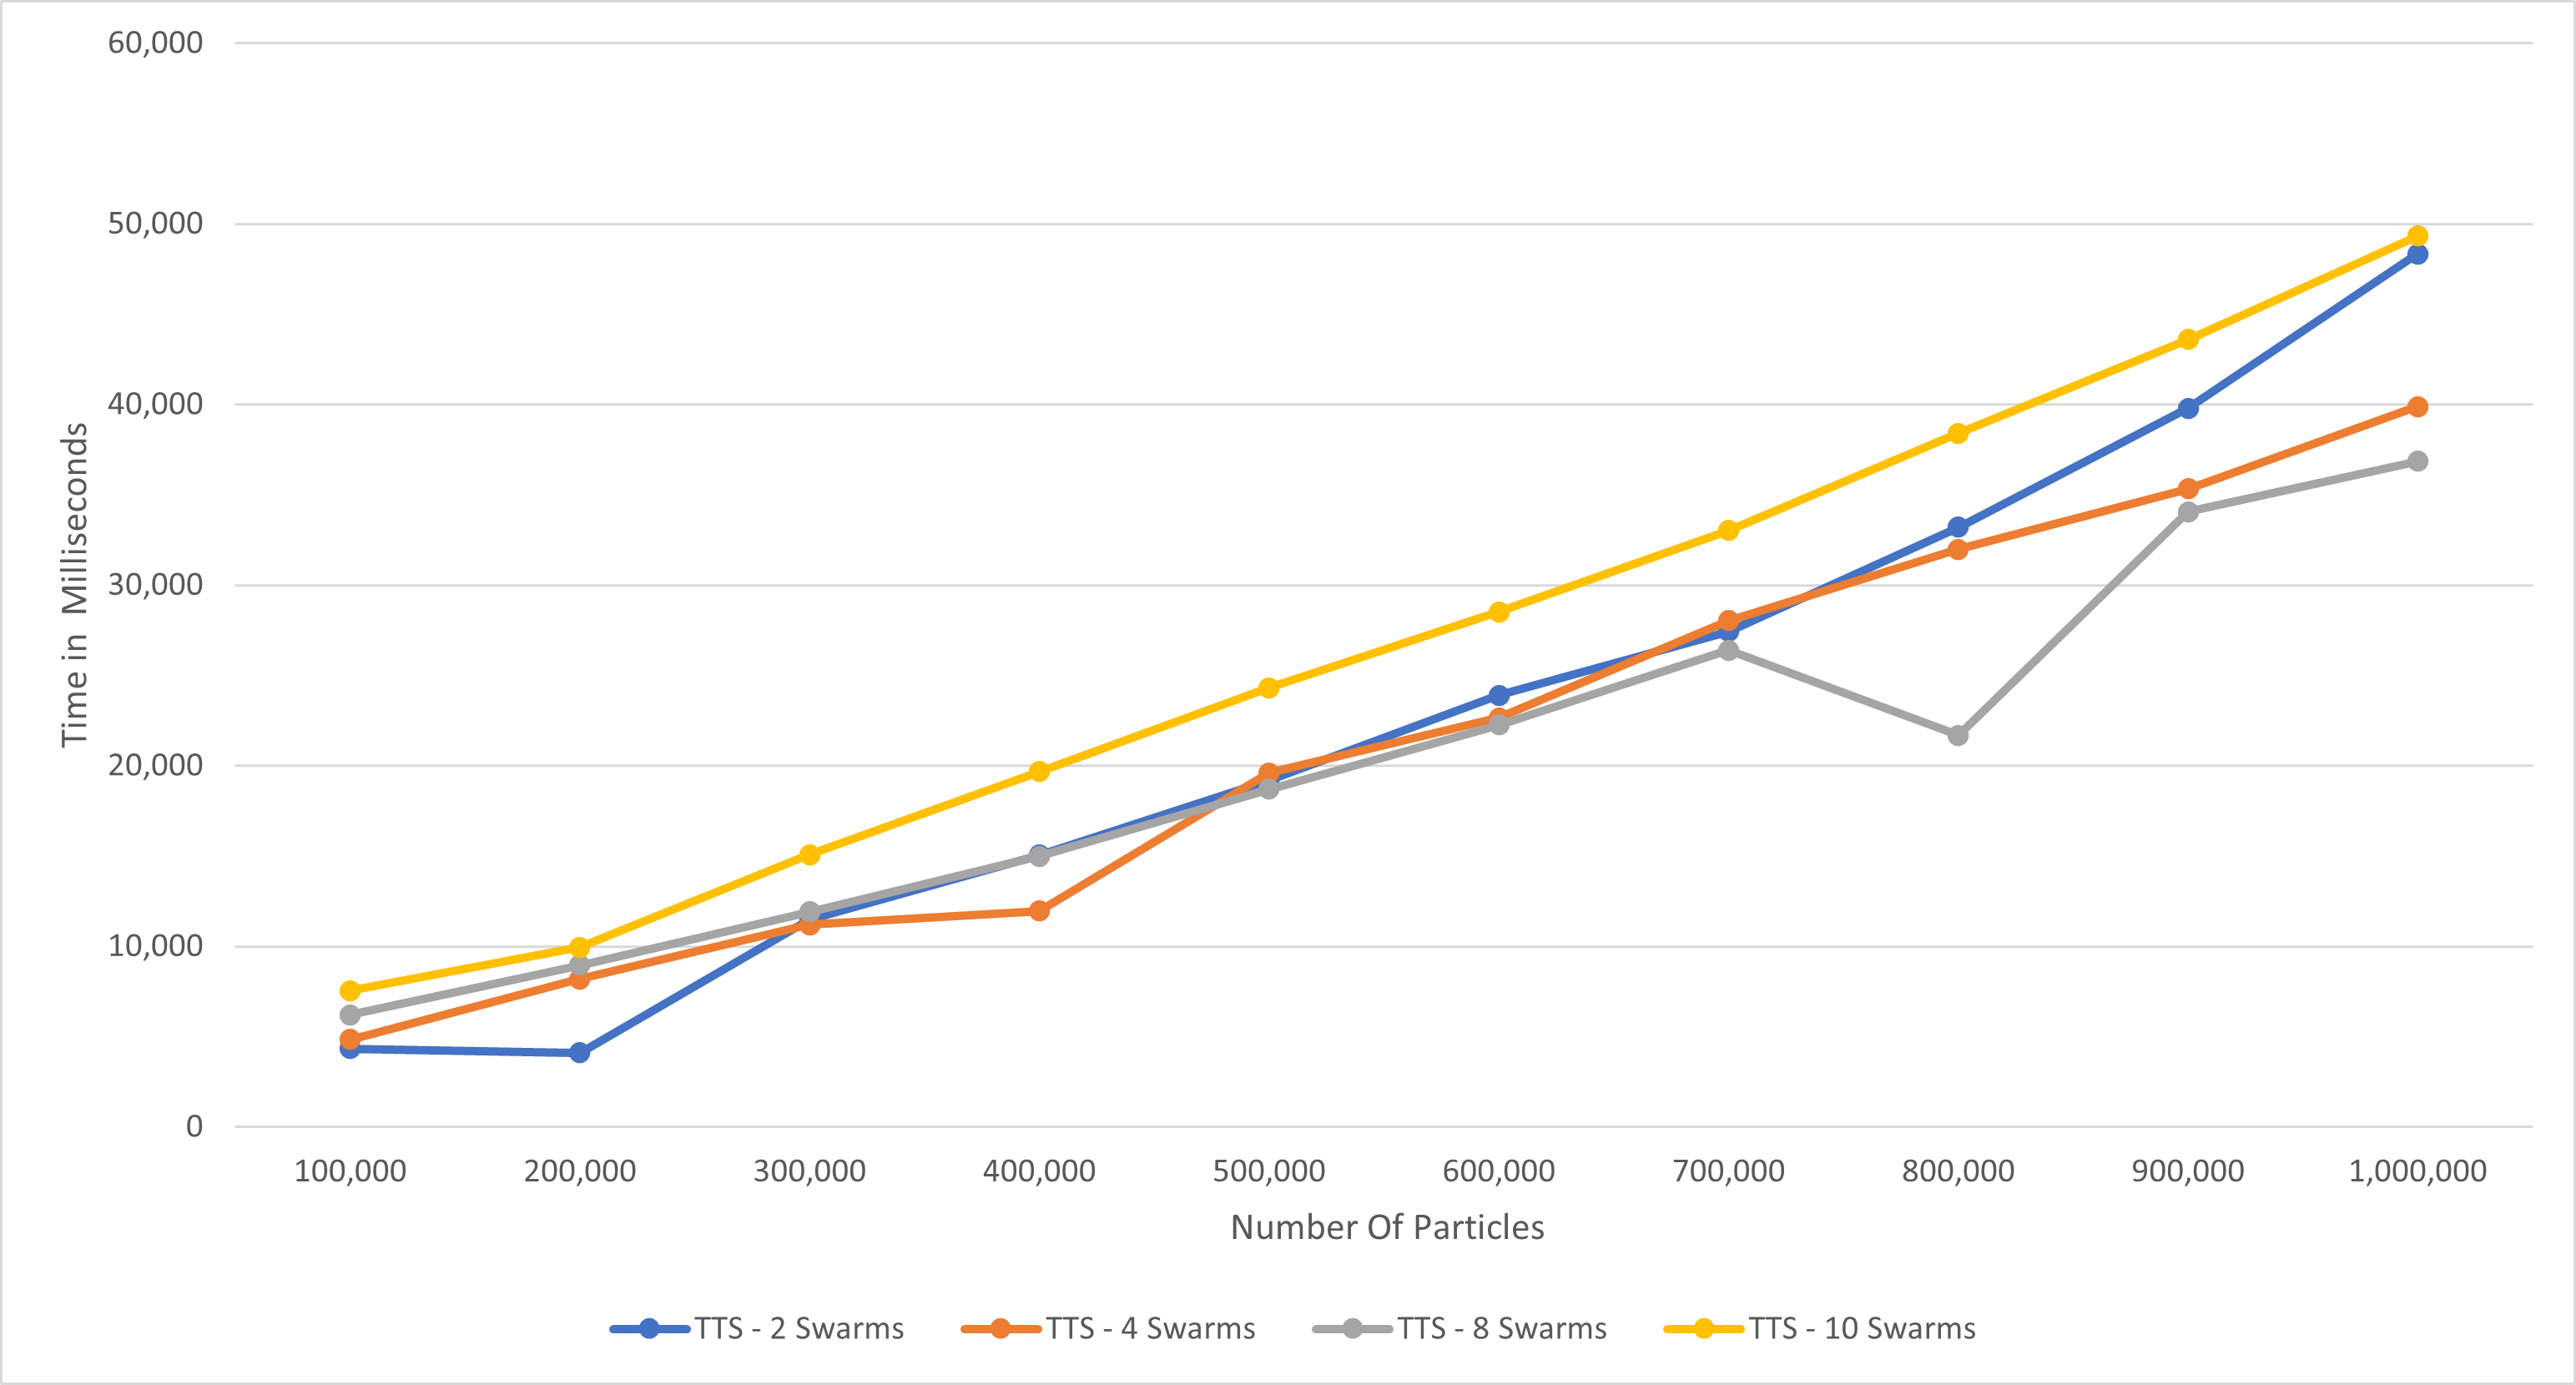
\includegraphics[scale=0.45]{Images/Graphs/DistributedBoothsTTS.png}
    \caption{Distributed TTS Booths Results}
    \label{fig:Distributed_TTS_Booths_Results}
\end{figure}

Figure \ref{fig:Distributed_Epoc_Booths_Results} shows the epochs to solution results. Unlike Easom results, the results are a bit more mixed. The two and ten swarm tests start off at a lower number of epochs at the beginning of the tests, with both starting at 108 iterations and ending at 117 iterations for ten swarms, and 114 iterations for the two swarm tests. Both the four and eight swarm tests show a more linear decrease, from start to finish, however both show a great deal of variance at various intervals in the testing. 

\begin{figure}[H]
    \centering
    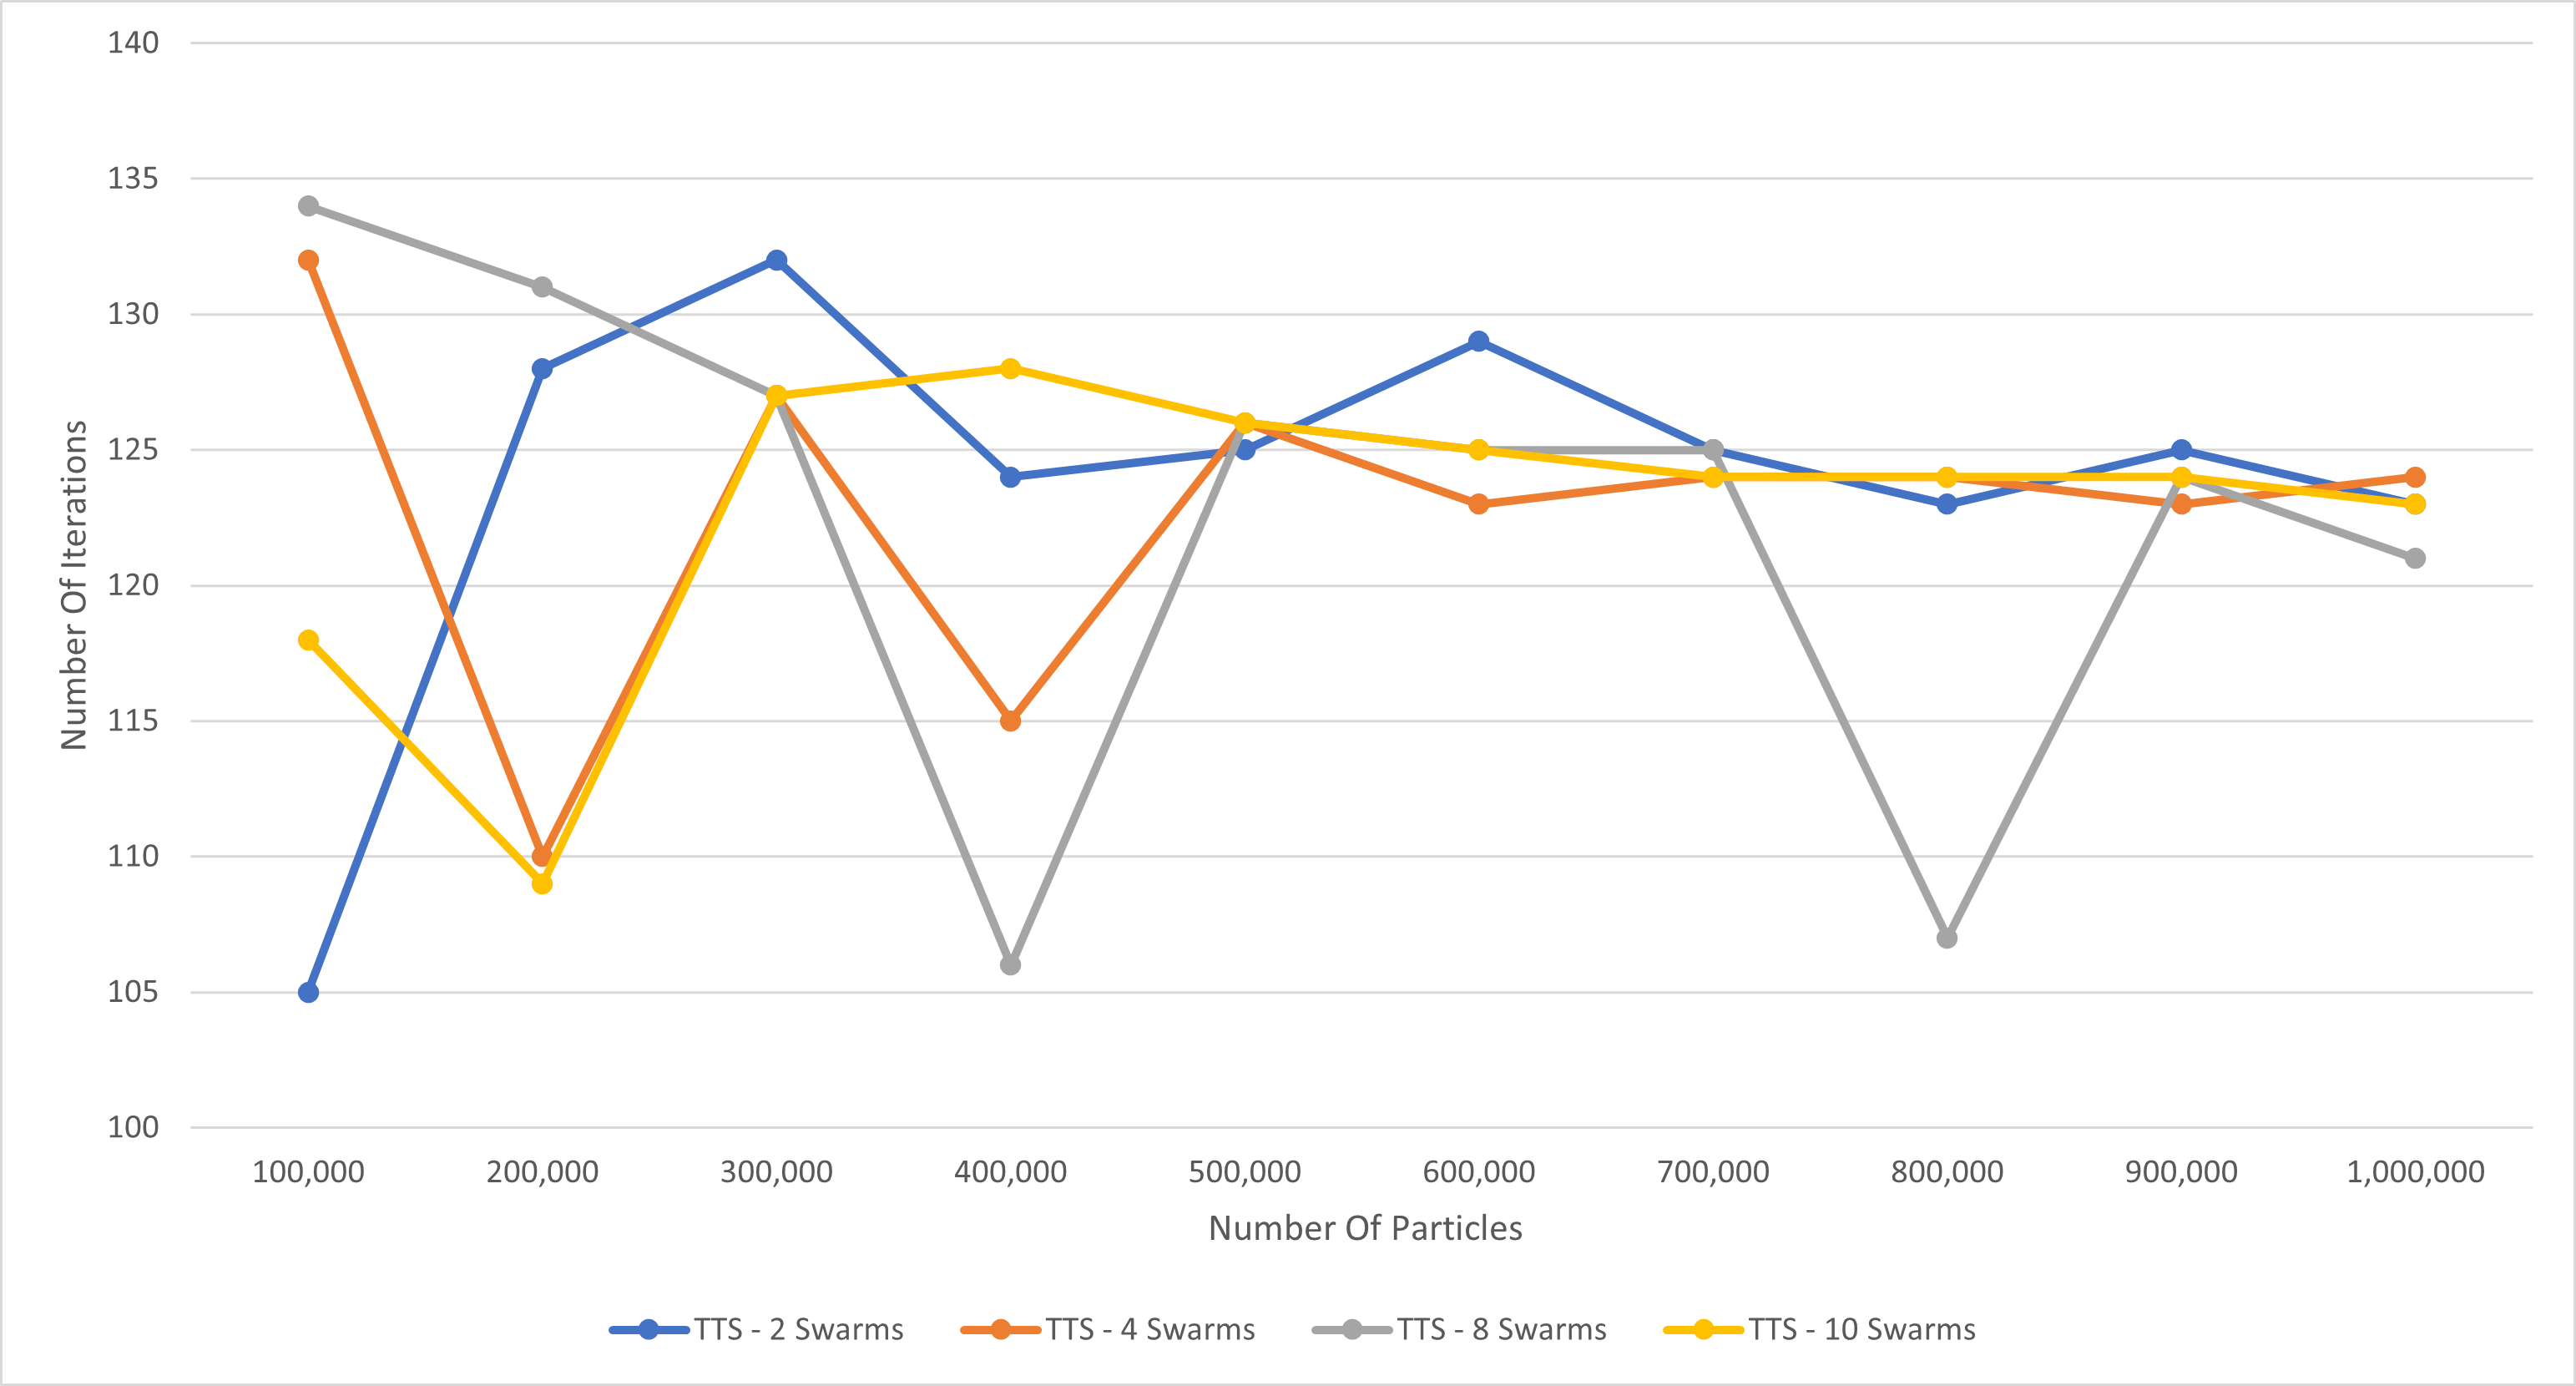
\includegraphics[scale=0.45]{Images/Graphs/DistributedBoothsEpoch.png}
    \caption{Distributed Iterations Booths Results}
    \label{fig:Distributed_Epoc_Booths_Results}
\end{figure}

\subsection{Beale Function}
Finally, looking at figure \ref{fig:Distributed_TTS_Beale_Results} we can see the TTS results for the Beale function. Again this follows the same trends as Booths and Easom functions, however its even less erratic, with little to no variance in the swam tests. Again the two swarm test runs show signs of it increasing at more than a linear increase at the higher number of particles, 900,000 and 1,000,000 particle tests. 
\begin{figure}[H]
    \centering
    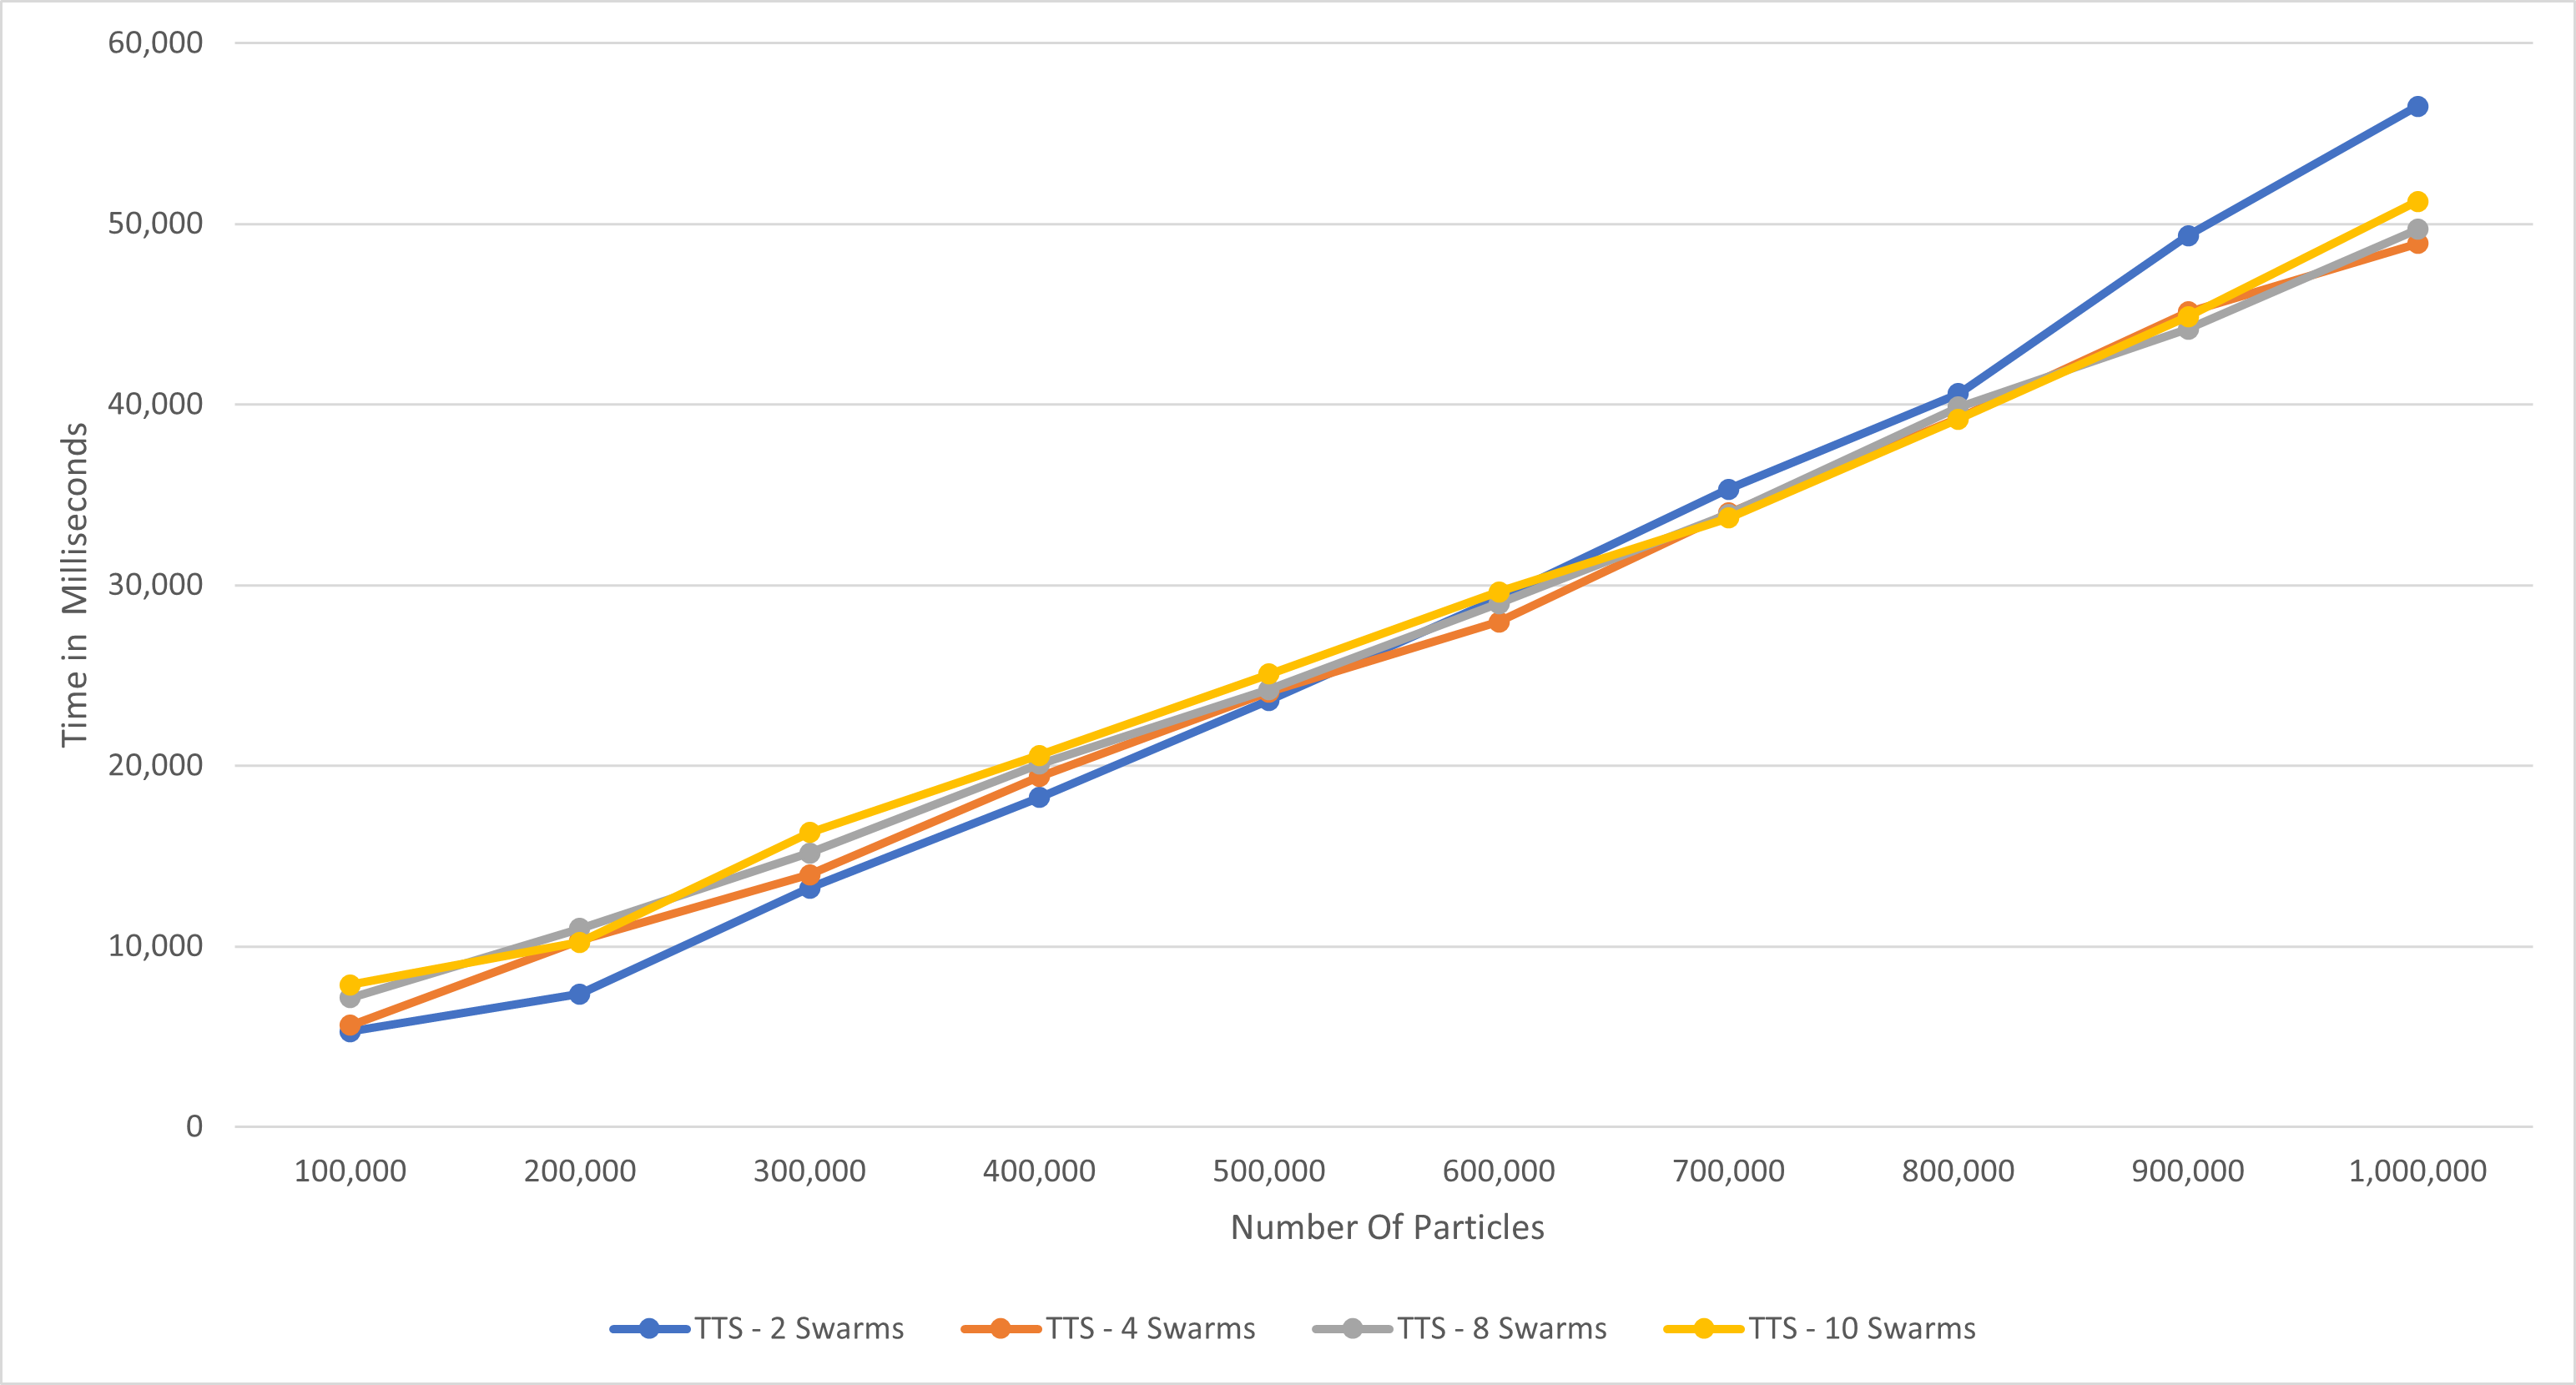
\includegraphics[scale=0.45]{Images/Graphs/DistributedBealeTTS.png}
    \caption{Distributed TTS Beale Results}
    \label{fig:Distributed_TTS_Beale_Results}
\end{figure}

Looking at figure \ref{fig:Distributed_Epoc_Beale_Results} we can see that once again the results show a great deal of variance when it comes to the number of epochs to reach a solution. Similar to the Booths function results, swarms two and ten start at a much lower number of epochs, but at the higher number of particles have much more similar results to the eight and four swarm results. Eight and four swarm results show a more gradual and consistent decline in epochs as the number of particles increases. 

\begin{figure}[H]
    \centering
    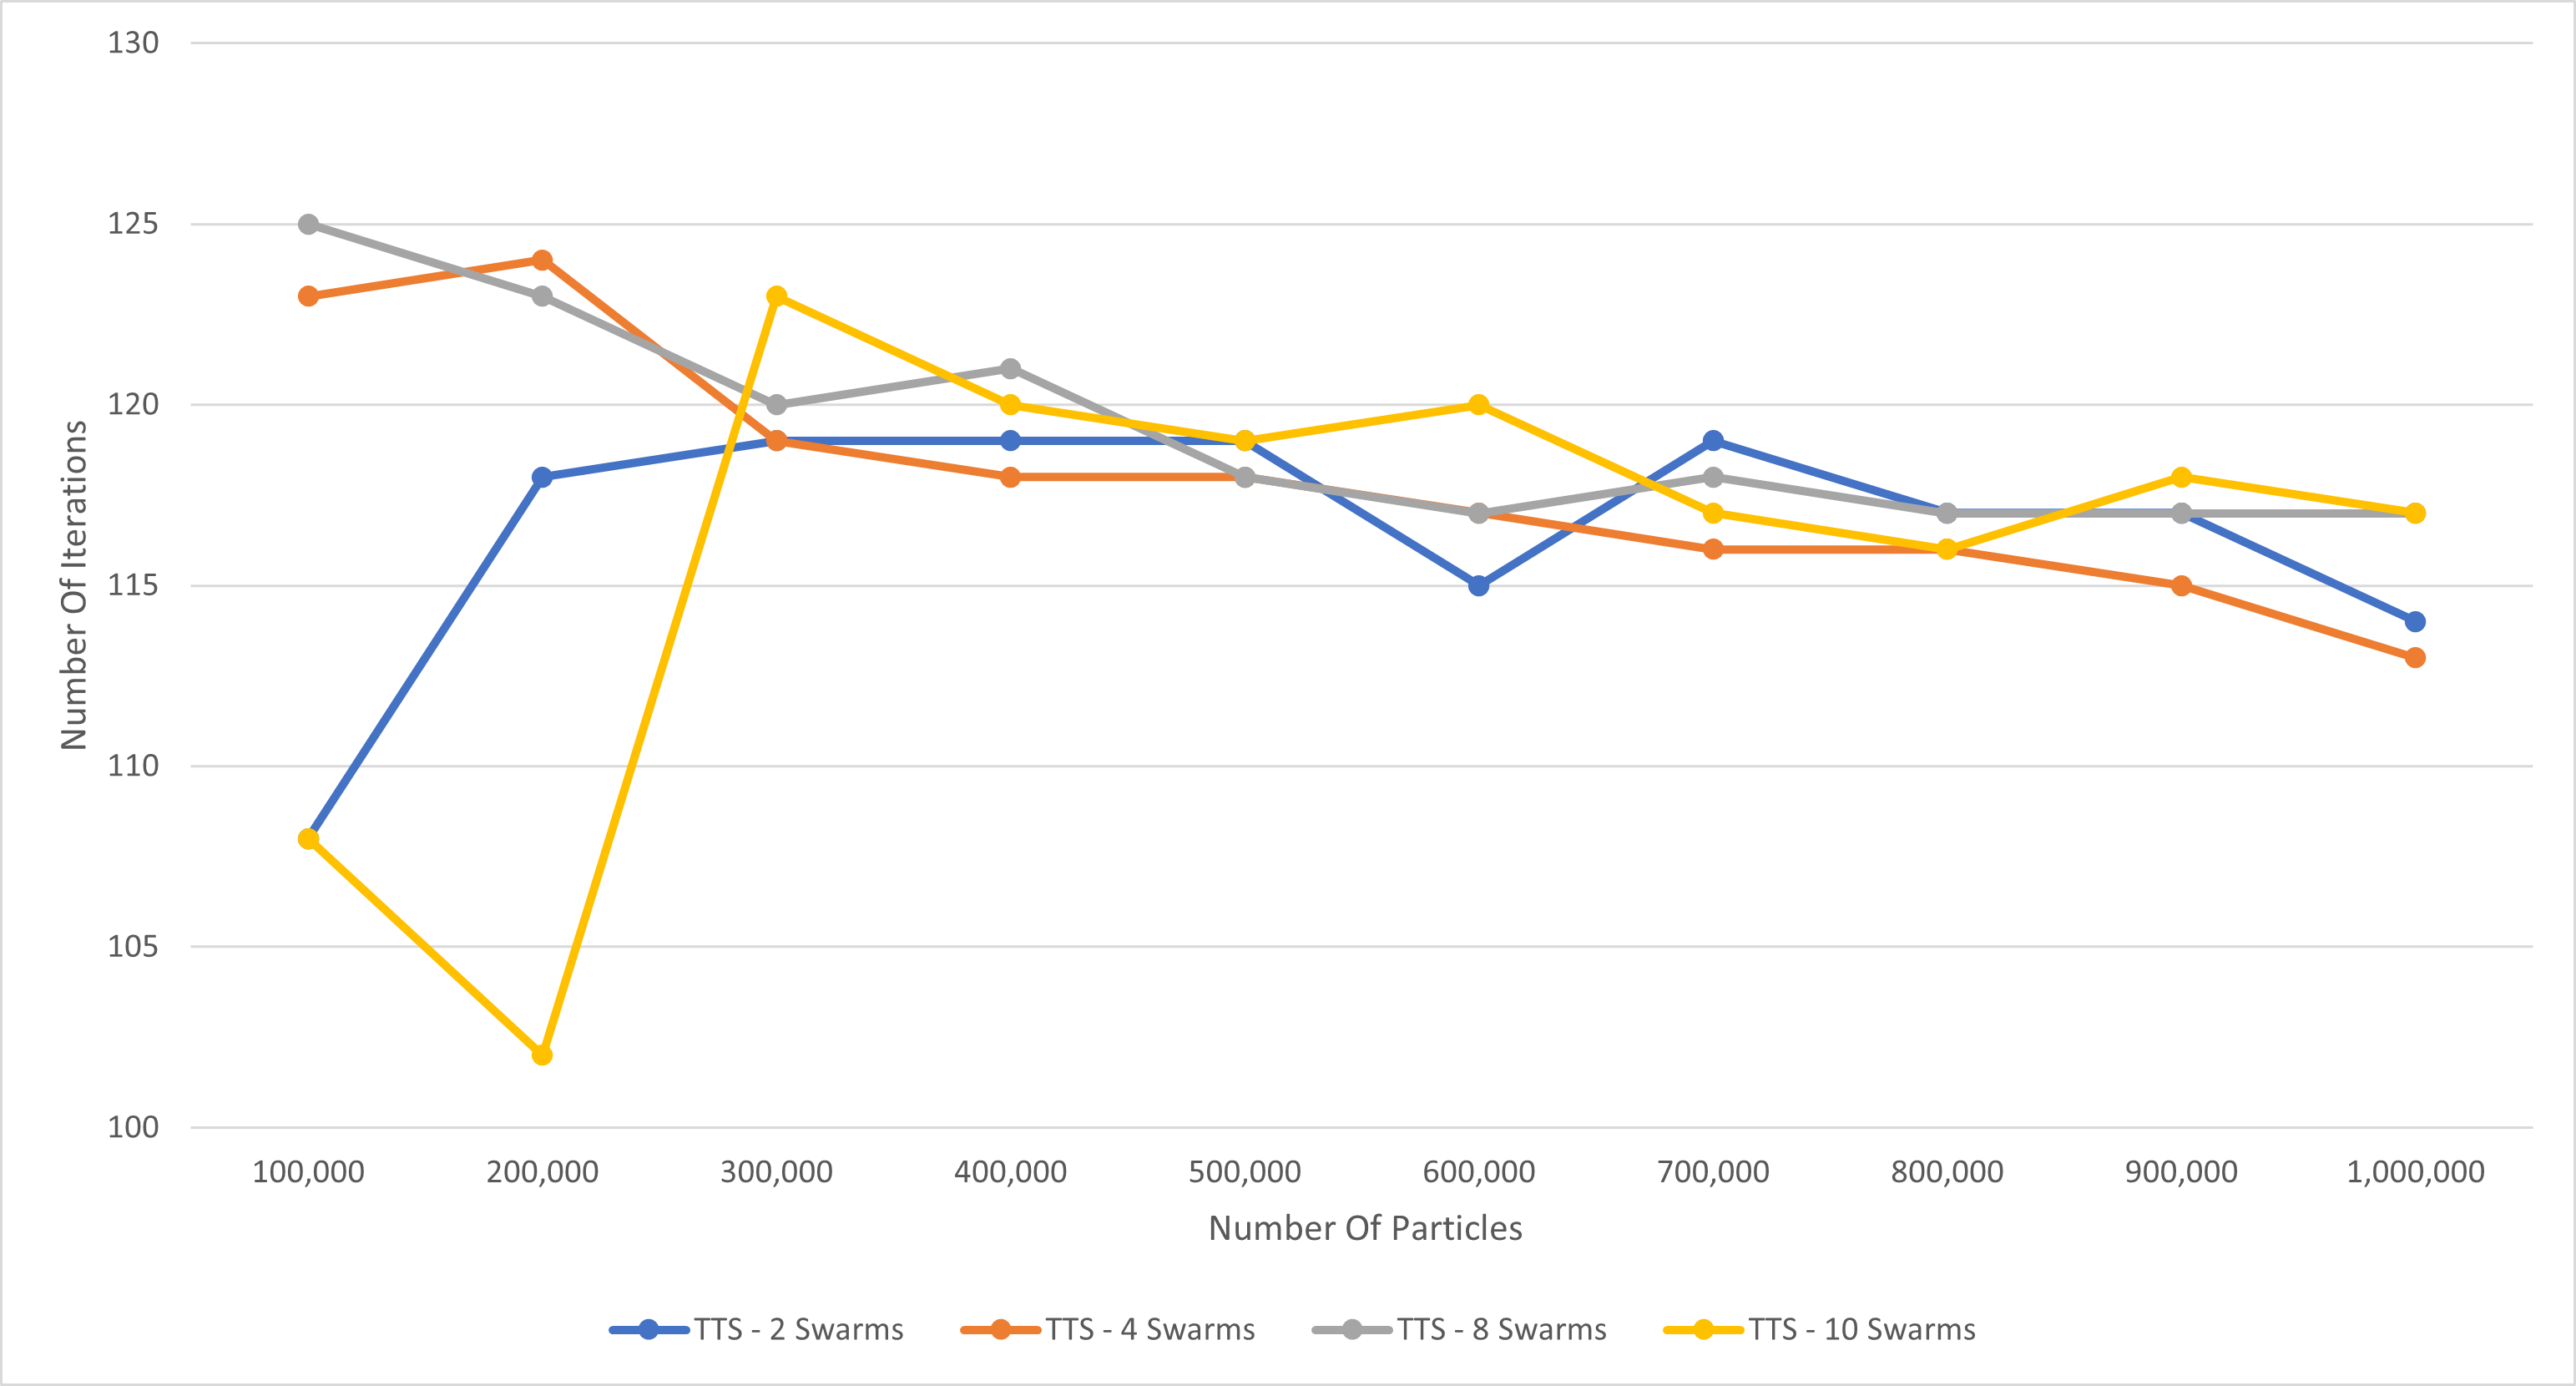
\includegraphics[scale=0.45]{Images/Graphs/DistributedBealeEpoch.png}
    \caption{Distributed Iterations Beale Results}
    \label{fig:Distributed_Epoc_Beale_Results}
\end{figure}

\section{Performance comparison}
Figure \ref{fig:PerformanceComparisonEasomTTS} displays a direct comparison between the distributed implementation of the Easom TTS results, and the centralised TTS results. This clearly displays the general trend of the centralised implementation towards an exponential increase, whereas the distributed implementation more closely follows a linear increase in TTS.  
\begin{figure}[H]
    \centering
    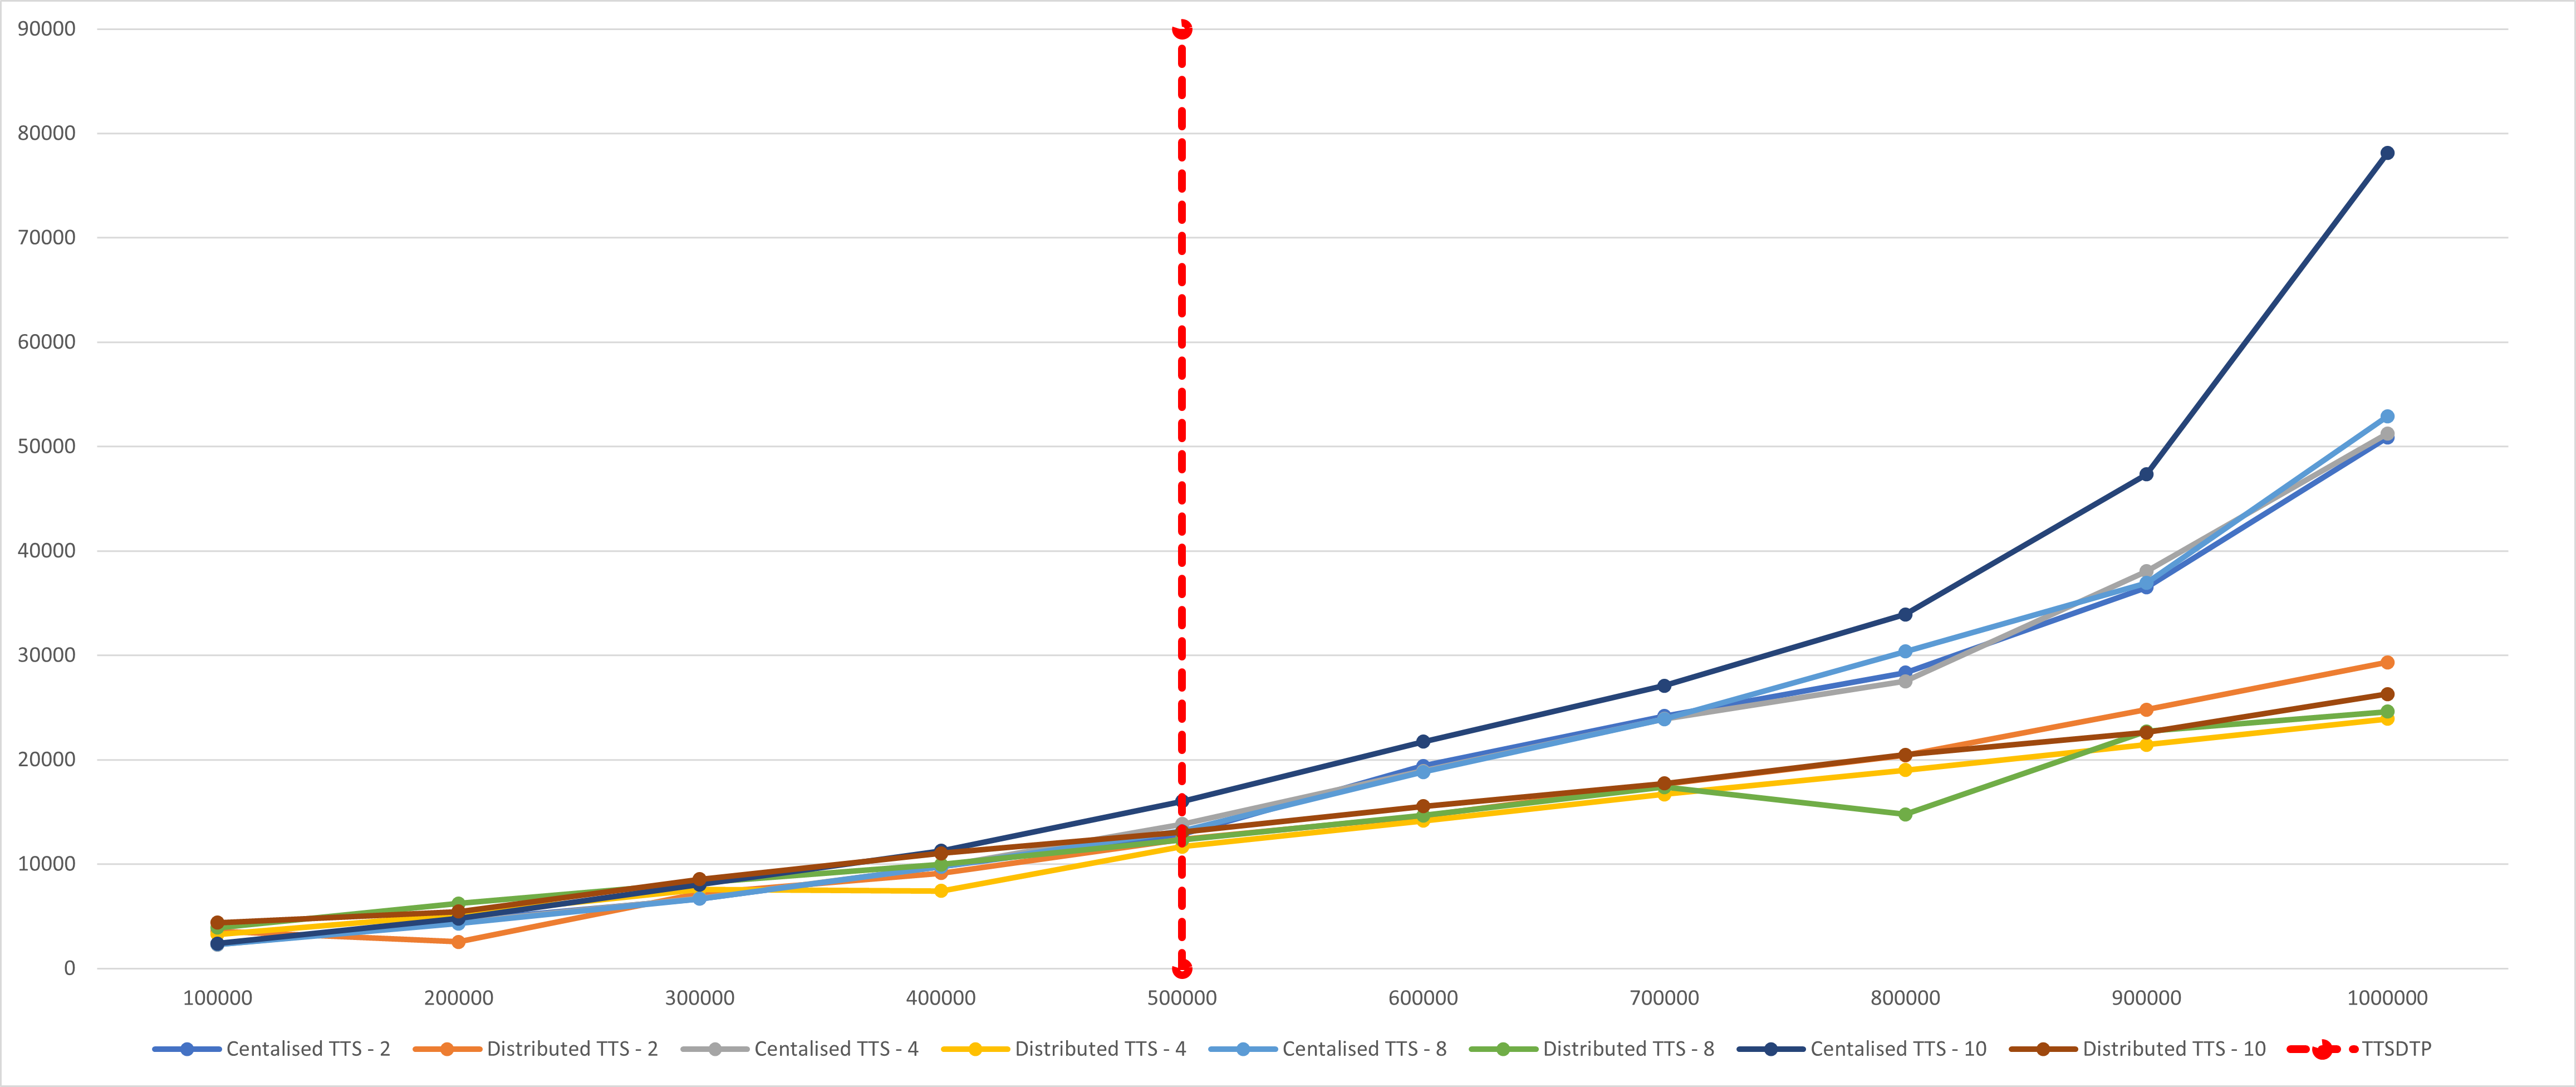
\includegraphics[scale=0.45]{Images/Graphs/PerformanceComparisonEasomTTS.png}
    \caption{Performance Comparison Easom TTS}
    \label{fig:PerformanceComparisonEasomTTS}
\end{figure}

Looking more closely at figure \ref{fig:PerformanceComparisonEasomTTS} we can see the two implementation seem to diverge in TTS increase rate at around five hundred thousand particles. This is more or less the same case in both Beale, figure \ref{fig:PerformanceComparisonBoothsTTS} and Booths function figure \ref{fig:PerformanceComparisonBealeTTS}. In all three results it shows the distributed implementation increasing at a linear rate, while the centralised implementations begins to increase exponentially after the five hundred thousand particles tests. There are other patterns observable in all three results, including the same tendency for two swarm tests in the centralised implementation to increase at a more rapid rate than other number of swarms at the higher number of particles tests. 

\begin{figure}[H]
  \centering
  \begin{minipage}[b]{0.48\textwidth}
    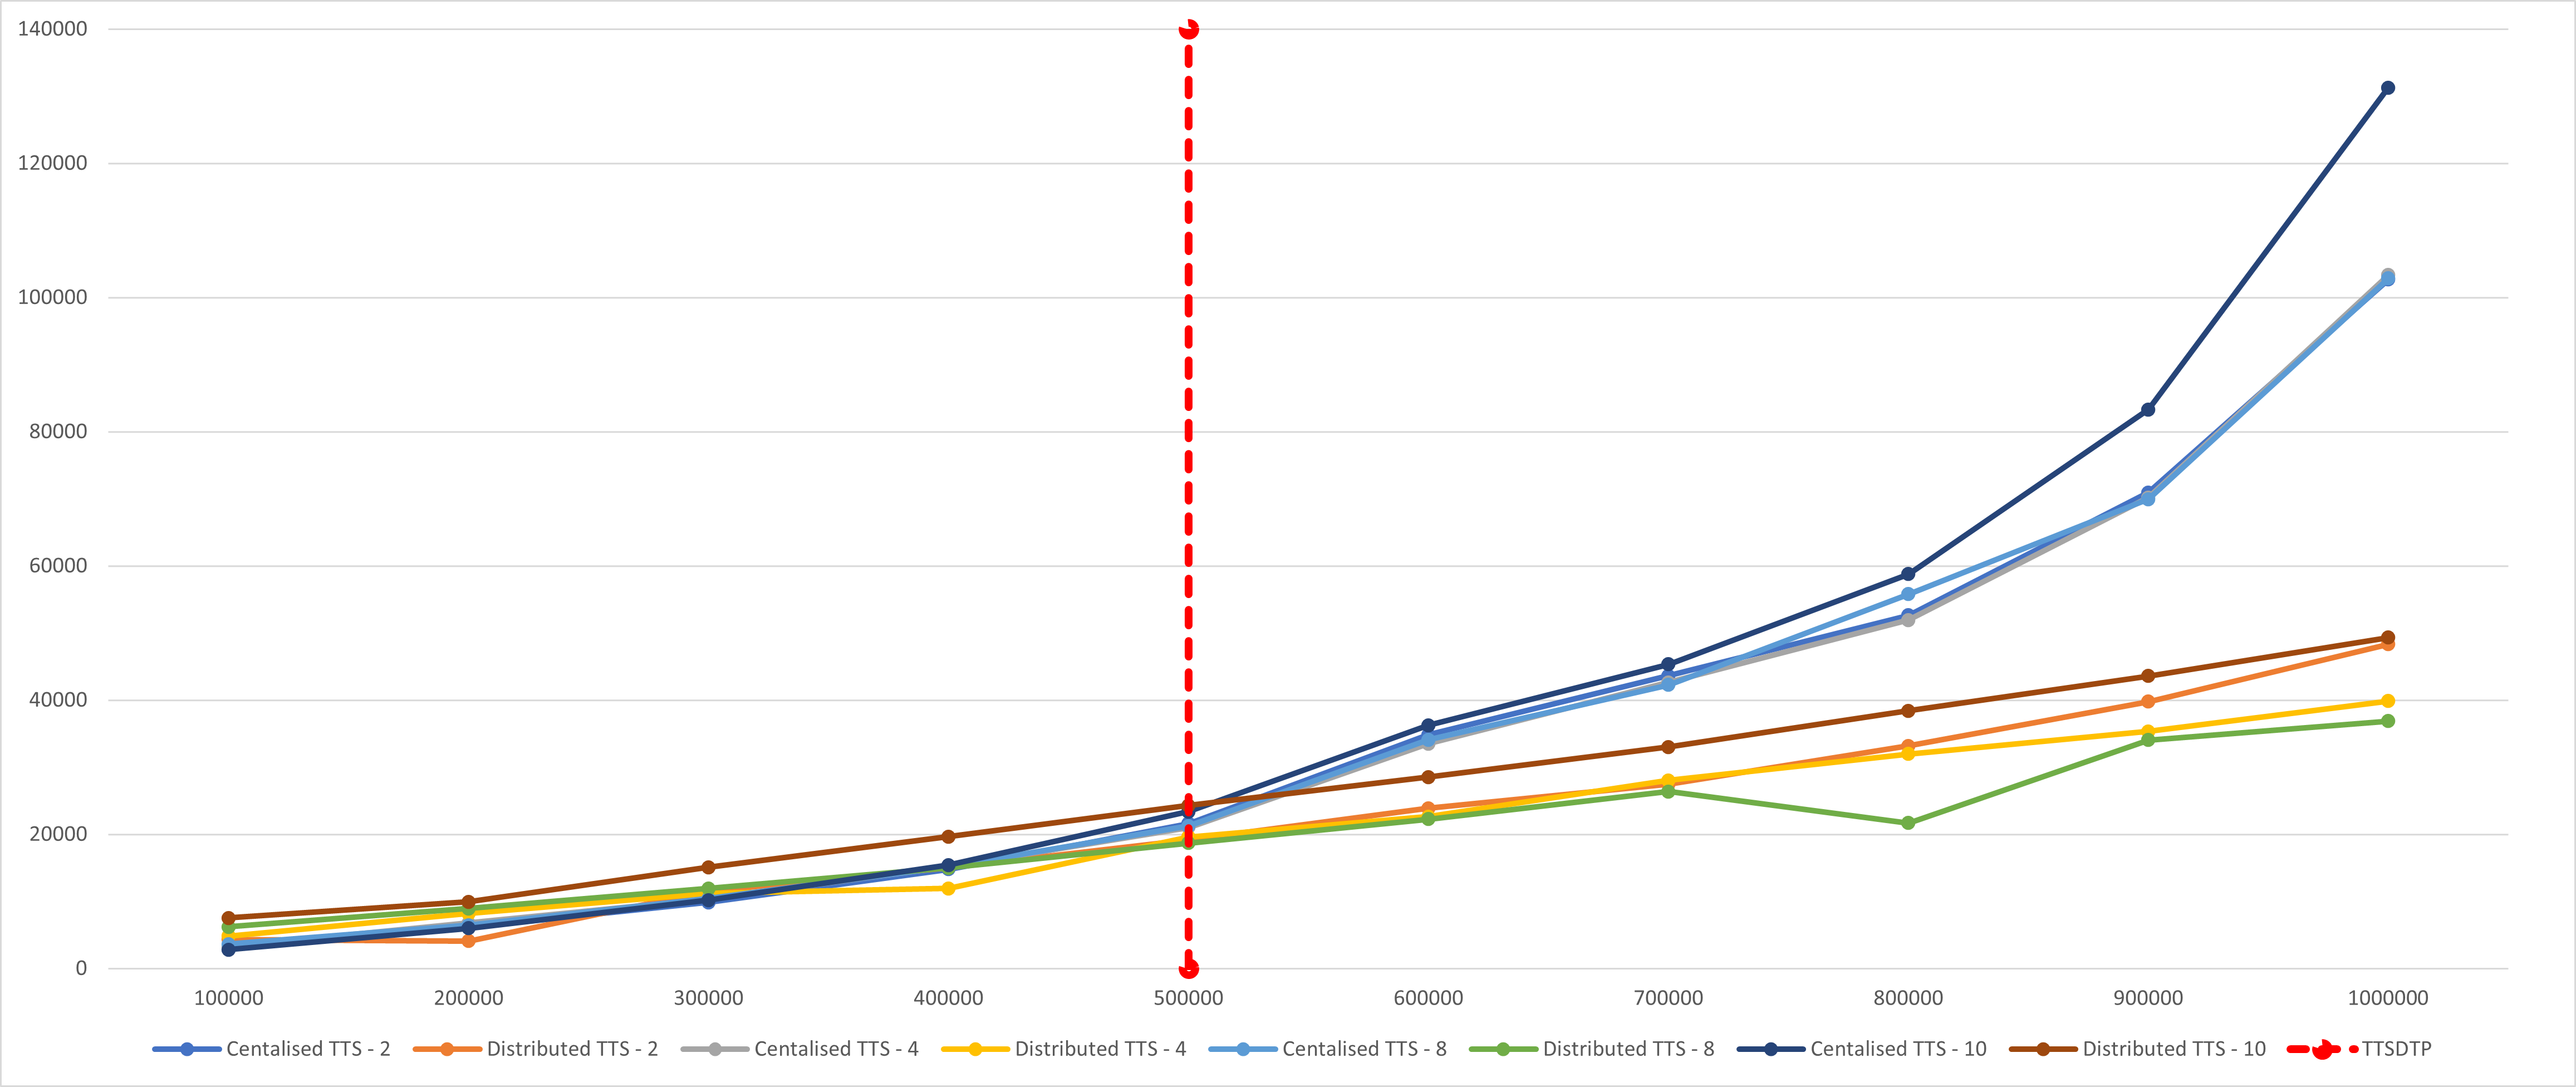
\includegraphics[width=\textwidth]{Images/Graphs/PerformanceComparisonBoothsTTS.png}
    \caption{Booths TTS comparison}
    \label{fig:PerformanceComparisonBoothsTTS}
  \end{minipage}
  \hfill
  \begin{minipage}[b]{0.48\textwidth}
    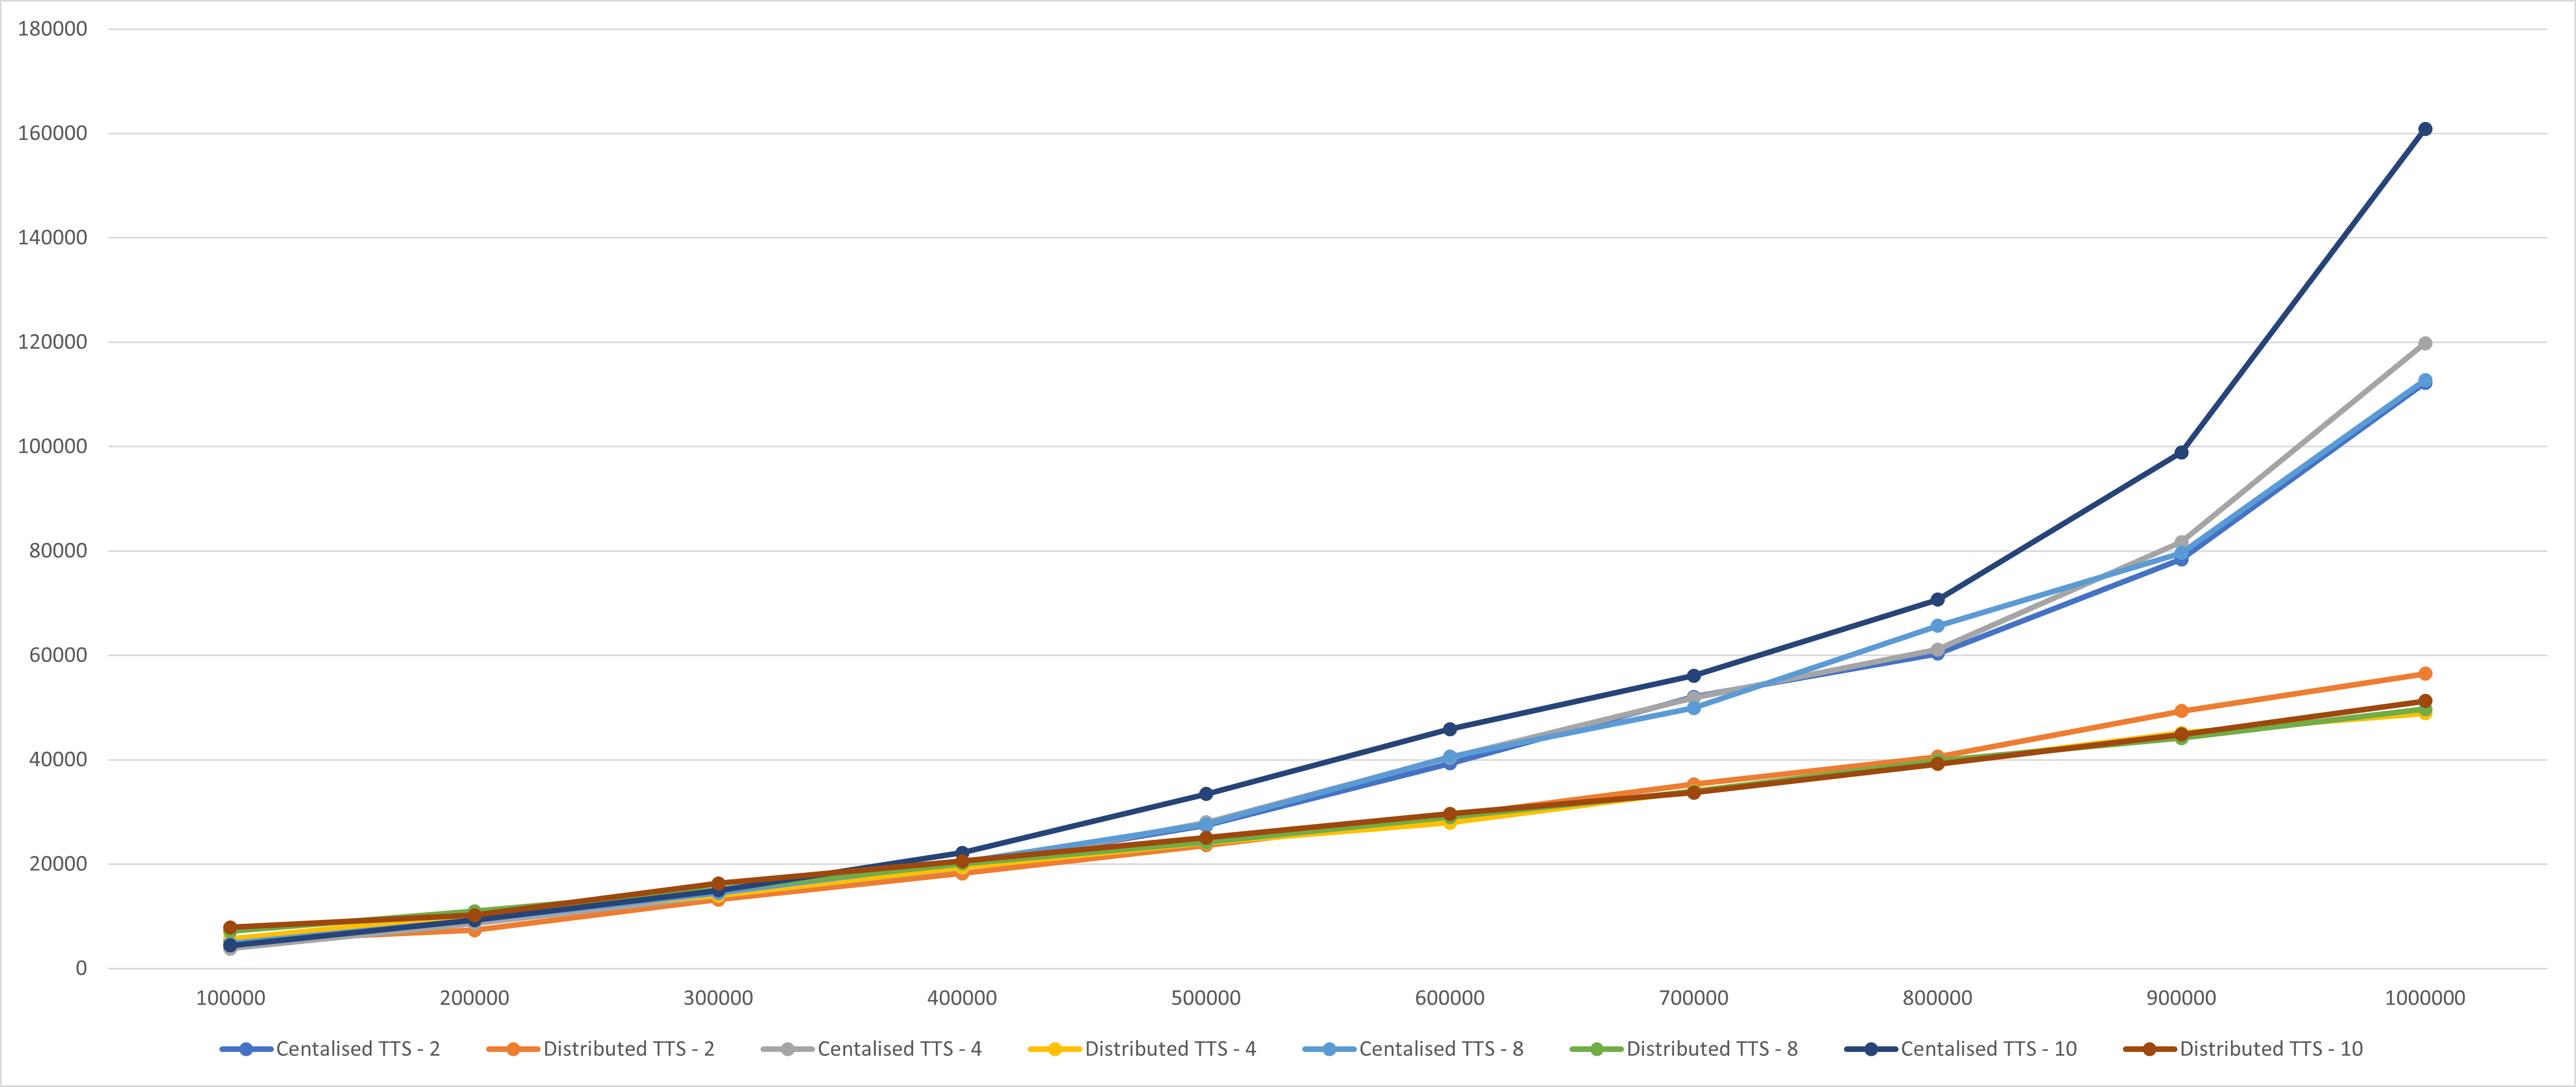
\includegraphics[width=\textwidth]{Images/Graphs/PerformanceComparisonBealeTTS.png}
    \caption{Beale TTS comparison}
    \label{fig:PerformanceComparisonBealeTTS}
  \end{minipage}
\end{figure}


All three functions display a large increase in TTS at the early stage of the experiment, with one hundred thousand particles. Table \ref{tab:TTSOneHundredThousand} compares these results. In the case of the Beale function, on average, the distributed implementation was 50\% slower at finding a result. Easoms function had an even greater increase, taking 61\% more time to find a solution, and Booths function was even bigger again, with it taking 82\% more time in finding a solution. 

% Table generated by Excel2LaTeX from sheet 'Test'
\begin{table}[H]
    \resizebox{\columnwidth}{!}{\begin{tabular}{|l|l|l|l|l|}
    \hline
          & \multicolumn{1}{l|}{\textbf{TTS - 2 Swarms}} & \multicolumn{1}{l|}{\textbf{TTS - 4 Swarms}} & \multicolumn{1}{l|}{\textbf{TTS - 8 Swarms}} & \multicolumn{1}{l|}{\textbf{TTS - 10 Swarms}} \\
    \hline
    \rowcolor[rgb]{ .851,  .882,  .949} \textbf{Beale -Centralised} & 4205  & 3842  & 4775  & 4417 \\
    \hline
    \rowcolor[rgb]{ .851,  .882,  .949} \textbf{Beale -Distributed} & 5291  & 5630  & 7153  & 7860 \\
    \hline
    \rowcolor[rgb]{ 1,  .949,  .8} \textbf{Booths -Centralised} & 2910  & 3243  & 3634  & 2805 \\
    \hline
    \rowcolor[rgb]{ 1,  .949,  .8} \textbf{Booths -Distributed} & 4331  & 4846  & 6197  & 7541 \\
    \hline
    \rowcolor[rgb]{ .886,  .937,  .855} \textbf{Easom -Centralised} & 2364  & 2297  & 2313  & 2388 \\
    \hline
    \rowcolor[rgb]{ .886,  .937,  .855} \textbf{Easom -Distributed} & 3551  & 3287  & 3925  & 4385 \\
    \hline
   \end{tabular}}%
  \caption{TTS Results for 100,000 Particles}    
  \label{tab:TTSOneHundredThousand}%
\end{table}%

Conversely there are some significant gains in TTS for the distributed implementation at the highest number of particles. Table \ref{tab:TTSOneMillion} compares these results for one million particle tests. For the Beale function it was found that the distributed implementation was on average 145\% faster than the centralised implementation. Similar performance gains where found with both Booths and Easom function, with Booths being 152\% faster, and Easom being 123\% faster. 


\begin{table}[H]
    \resizebox{\columnwidth}{!}{\begin{tabular}{|l|l|l|l|l|}
    \hline
    & \multicolumn{1}{l|}{\textbf{TTS - 2 Swarms}} & \multicolumn{1}{l|}{\textbf{TTS - 4 Swarms}} & \multicolumn{1}{l|}{\textbf{TTS - 8 Swarms}} & \multicolumn{1}{l|}{\textbf{TTS - 10 Swarms}} \\
    \hline
    \rowcolor[rgb]{ .851,  .882,  .949} \textbf{Beale -Centralised} & 112258 & 119800 & 112751 & 160899 \\
    \hline
    \rowcolor[rgb]{ .851,  .882,  .949} \textbf{Beale -Distribributed} & 56502 & 48906 & 49696 & 51248 \\
    \hline
    \rowcolor[rgb]{ 1,  .949,  .8} \textbf{Booths -Centralised} & 102709 & 103364 & 102856 & 131270 \\
    \hline
    \rowcolor[rgb]{ 1,  .949,  .8} \textbf{Booths -Distribributed} & 48322 & 39878 & 36861 & 49330 \\
    \hline
    \rowcolor[rgb]{ .886,  .937,  .855} \textbf{Easom -Centralised} & 50887 & 51263 & 52918 & 78160 \\
    \hline
    \rowcolor[rgb]{ .886,  .937,  .855} \textbf{Easom -Distribributed} & 29327 & 23923 & 24623 & 26300 \\ \hline
   \end{tabular}}%
  \caption{TTS Results for 1,000,000 Particles}    
  \label{tab:TTSOneMillion}%
\end{table}%

When looking at the number of iterations between the two implementations there is very little difference the two. Looking at figures; \ref{fig:PerformanceComparisonEasomEpoch}, \ref{fig:PerformanceComparisonBoothsEpoch}, \ref{fig:PerformanceComparisonBealeEpoch}, we can see the same general trends in all three fitness functions. There is an overall gradual decline in iterations as particles increase, with some large variations, especially at the lower end of the particles. Overall the distributed implementations showed more variations than the centralised implementations. 

\begin{figure}[H]
    \centering
    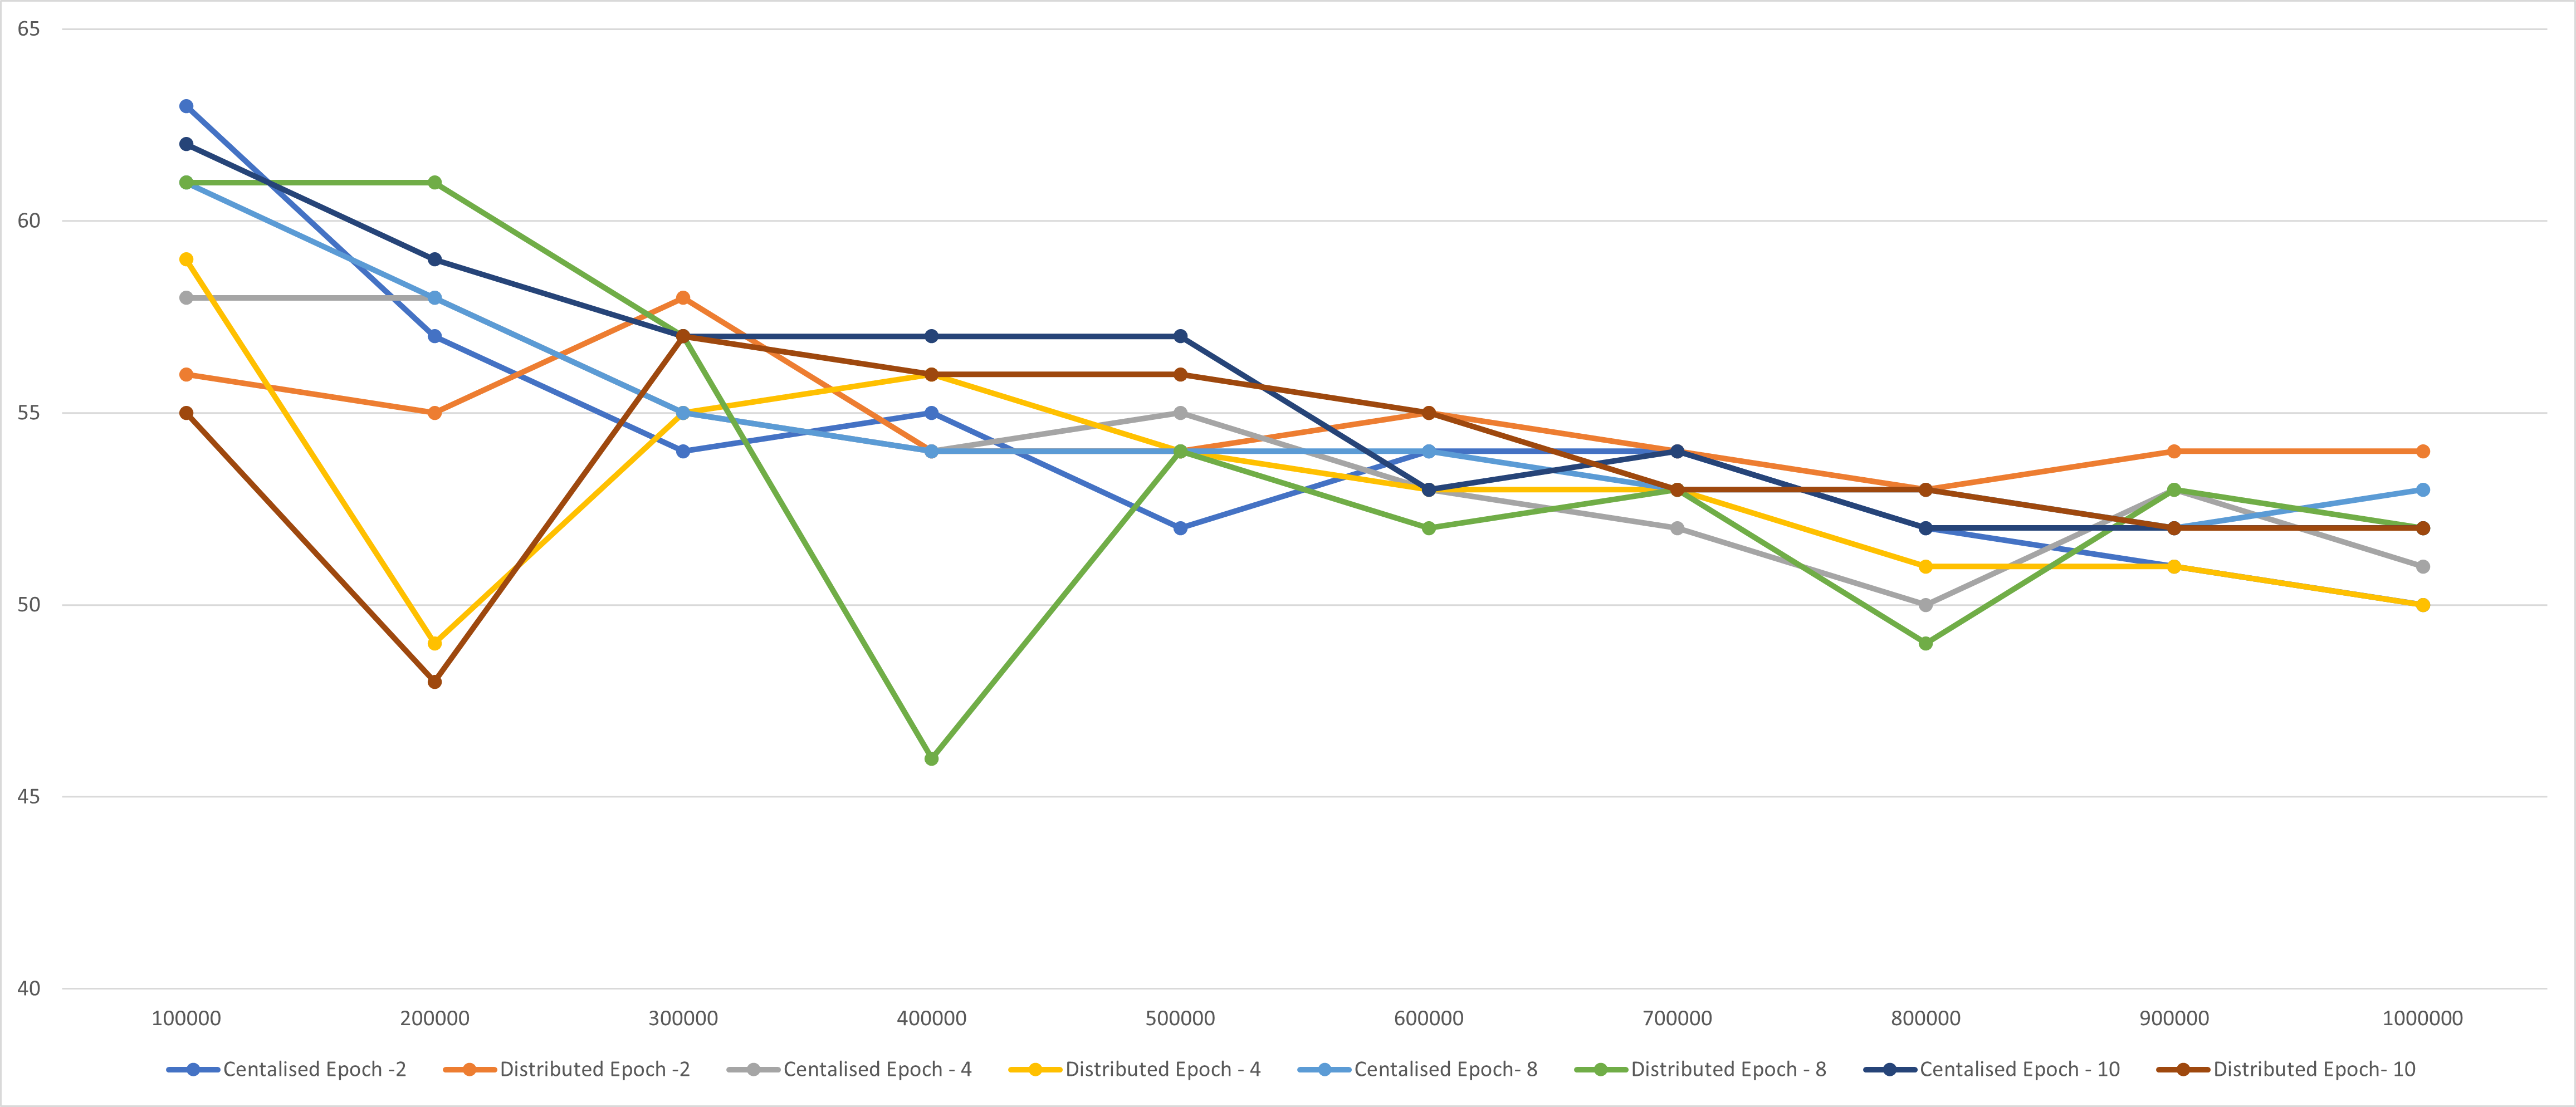
\includegraphics[scale=0.45]{Images/Graphs/PerformanceComparisonEasomEpoch.png}
    \caption{Performance Comparison Easom Epoch}
    \label{fig:PerformanceComparisonEasomEpoch}
\end{figure}

\begin{figure}[H]
  \centering
  \begin{minipage}[b]{0.48\textwidth}
    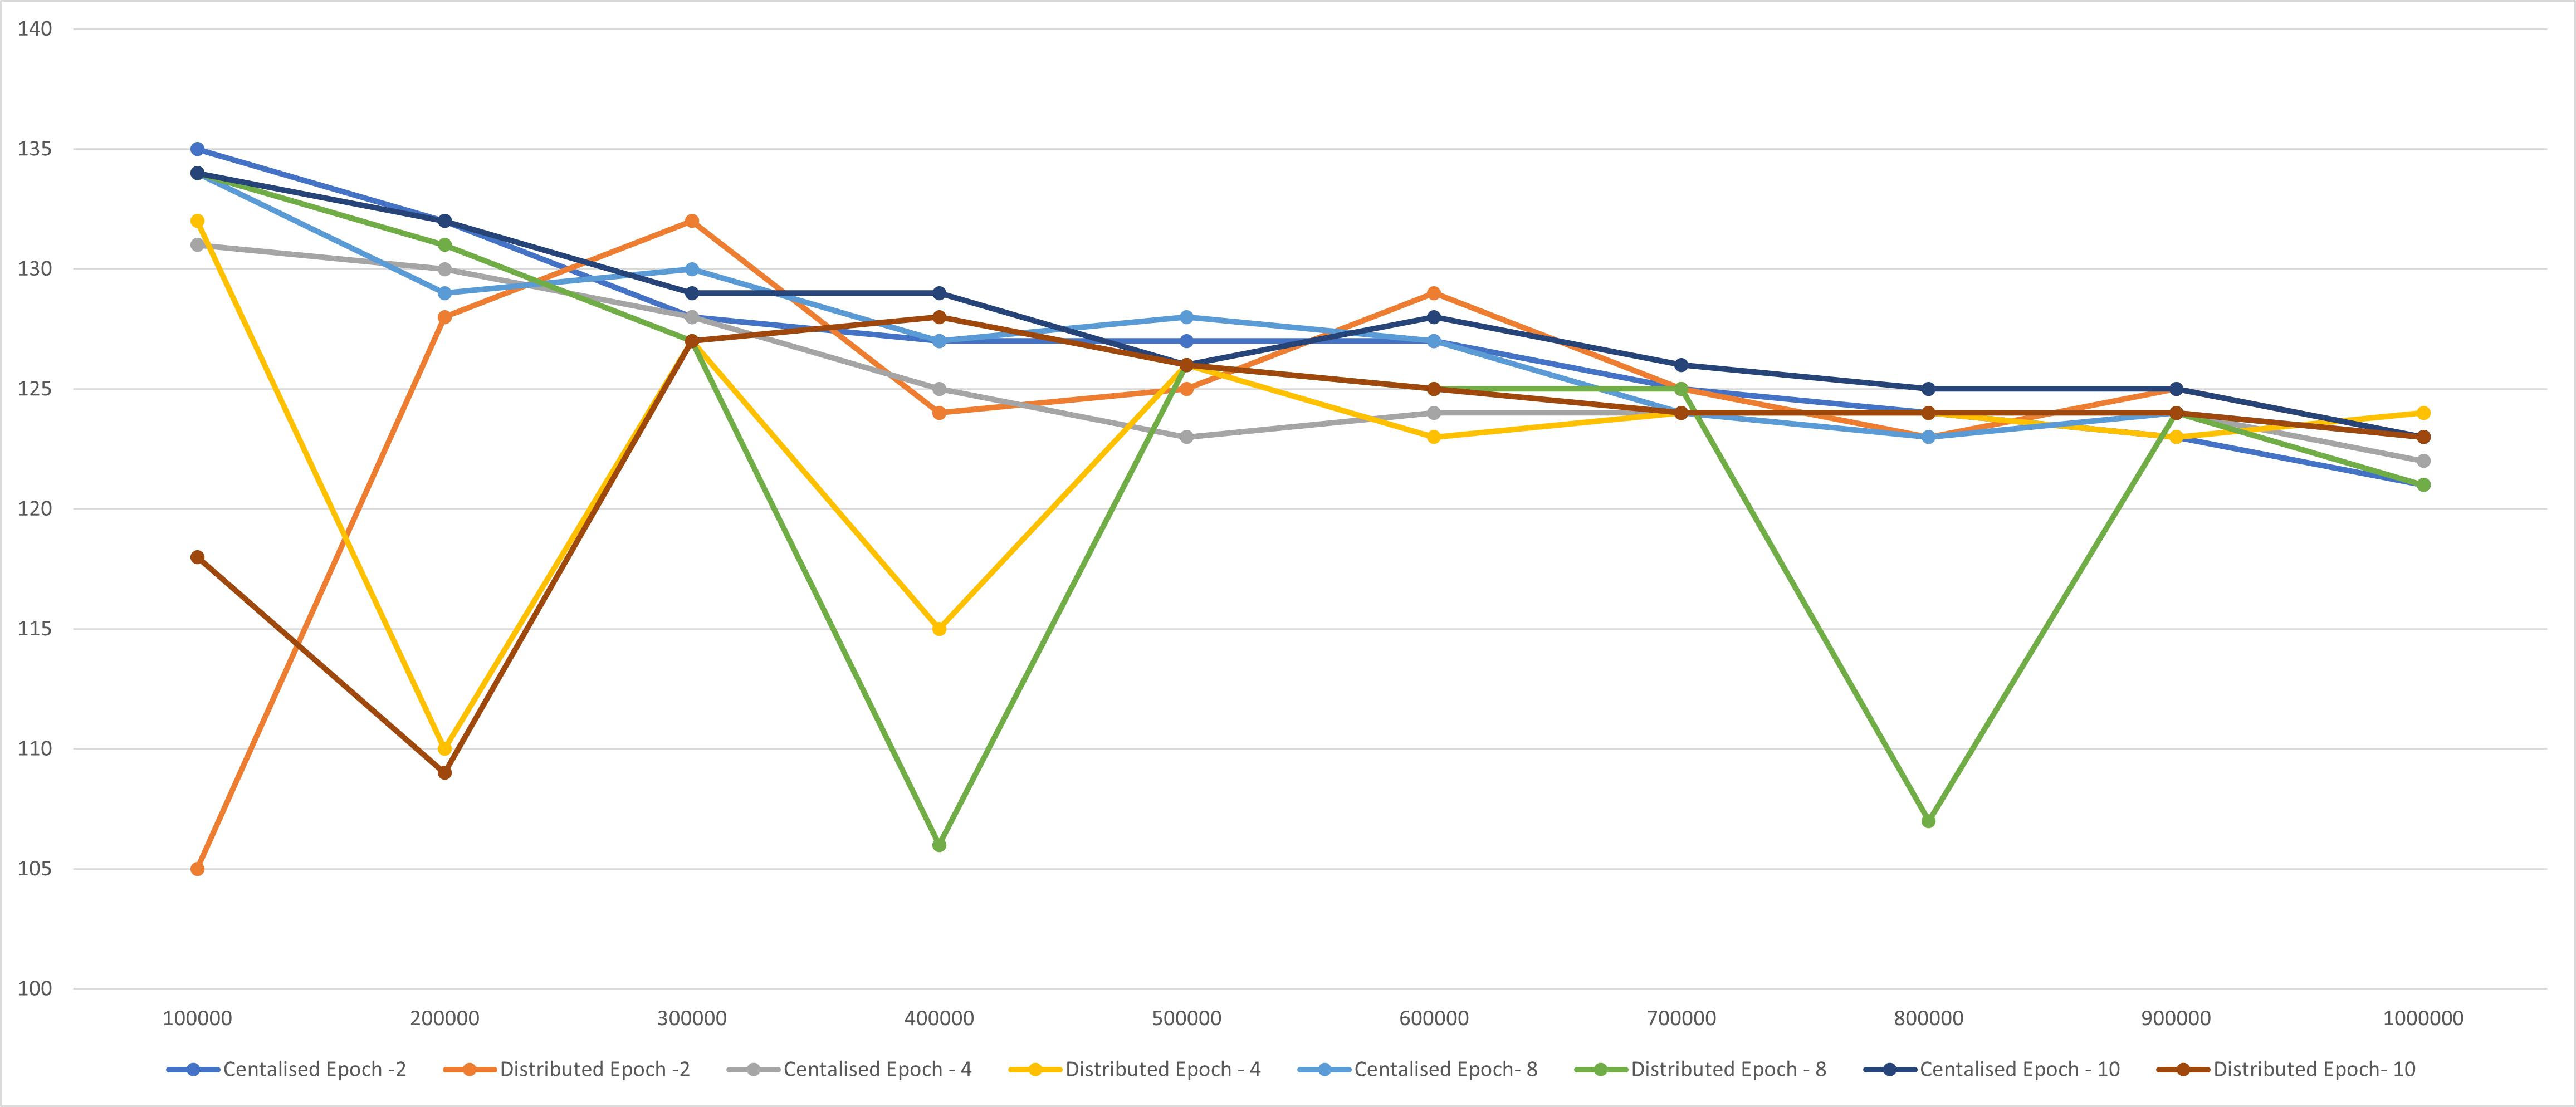
\includegraphics[width=\textwidth]{Images/Graphs/PerformanceComparisonBoothsEpoch.png}
    \caption{Booths Epoch comparison}
    \label{fig:PerformanceComparisonBoothsEpoch}
  \end{minipage}
  \hfill
  \begin{minipage}[b]{0.48\textwidth}
    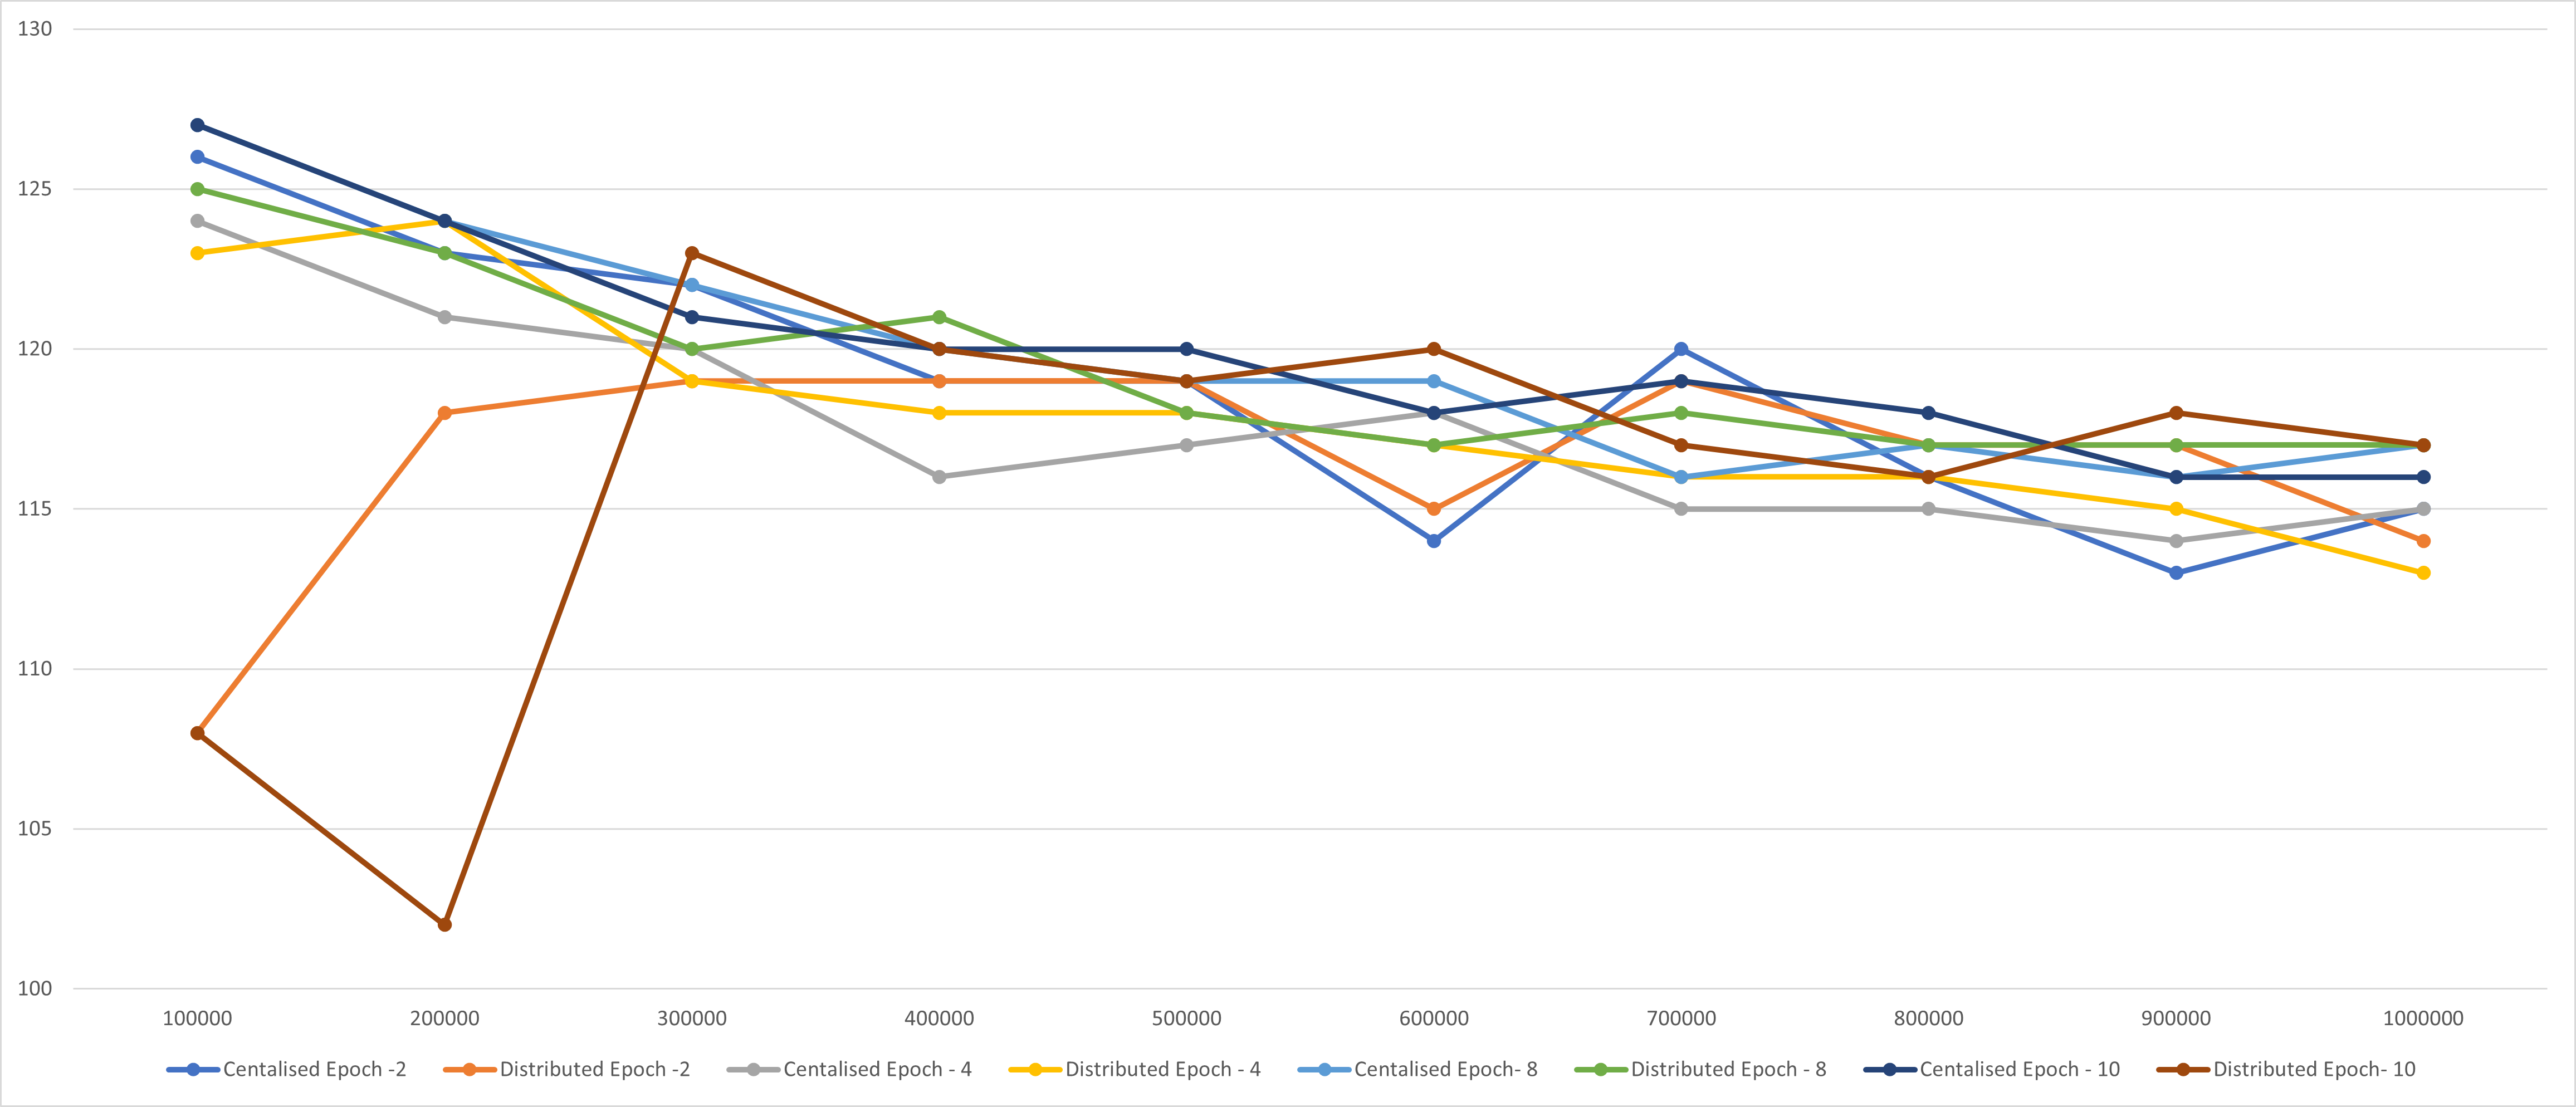
\includegraphics[width=\textwidth]{Images/Graphs/PerformanceComparisonBealeEpoch.png}
    \caption{Beale Epoch comparison}
    \label{fig:PerformanceComparisonBealeEpoch}
  \end{minipage}
\end{figure}

\section{Results Evaluation}
From the performance comparison section we can see there is a clear point in all three fitness functions whereby the distributed implementation displays a better time to solution than the centralised implementation. Interestingly, for all three this occurs at more or less the same point. Once the number of particles across all swarms reaches 500,000 or greater, the distributed implementation begins to be a more efficient implementation than the centralised implementation. Once the particles reach one million all three functions had a greater than 100\% decreases in time to solution compared to the corresponding centralised tests.

This clearly answers the research question, that there is in fact a point whereby it is more efficient to run a distributed PSO implementation over a centralised implementation. However, this must be caveated by the fact that these results are only a guide, a different fitness function may have a different efficiency point. Additionally different implementation languages, or PSO implementation methods may also have different efficiency points. 
We can therefore conclude that the alternate hypothesis has been proven, and there is a point where a distributed implementation is more time efficient than a centralised implementation. 

In terms of differences between the number of iterations taken before finding a solution, between the two implementations, this study found no difference between the distributed implementation and the centralised implementation. There was a noticeable decline in the number of iterations across both implementations as the number of particles increased, and this was evident across all three fitness functions. When looking at other resulting data points, such as the average x/y value, and final group best, this study found no difference between the implementation, and no differences as the number of particles increase. The number of particles used in this study can be considered overkill, as the number of particles required to correctly find a solution to any of the fitness functions was significantly lower than what was used in this study. However, as matching the trend seen in both implementations, the lower number of particles required much more iterations to find a "settled" solution. 


\section{Conclusion}
This chapter covered in-depth the results obtained from running the experiment described in chapters three and four. Each implementations results where presented, subdivided by the individual fitness function tested. Commentary was provided on these results, with some notable trends highlighted. 
Distributed implementation results and centralised results where also compared together, highlighting some interesting trends within the results, including a tendency for centralised TTS results to increase exponentially, whereas the distributed TTS results appeared to increase at a more linear rate. The research question was answered, and the alternate hypthosis was accepted, in that there is a point whereby a distributed PSO implementation becomes more efficient than a centralised implementation. It was noted that across both implementations there was a general trend of decreasing the total number of epochs required to reach a solution as the number of particles increased.

The next chapter will conclude this research, with an overview of what has been accomplished in this experiment, evaluation of the results found from the experiment, and some future work and recommendations will be discussed. 


% Concluding chapter
% ============================================================= %
\chapter{Conclusion}
This chapter summarises the entire research project, reviewing the research objective and presents the answer to the research question. Finally the contribution, impact and future work \& recommendations are presented and discussed. 

\section{Research Overview}
This study aimed to find empirical evidence that there was a point whereby its  more  efficient  to  run a particle swarm optimisation algorithm in a distributed manner over a centralised implementation. Chapter one introduced the research topic, and some basic overview of the research piece. Chapter two presented research into the PSO topic, and identified a gap in the literature around PSO, that being that no existing literature focused on the point where a distributed PSO implementation is more time efficient than a centralised implementation. This gap was used to form the basis of this research topic. Chapter three and four discussed the experiment design and implementation, with some details provided on how to run the experiment and how the results data set was obtained. Finally chapter five concluded with an overview of the results obtained and some interesting trends seen within the results data set. 

\section{Problem Definition}
The aim of the research was to find a point where a distributed particle implementation became more time efficient than a centralised implementation, once the number of swarms or particles hits a particular level. This formed the research question ”At what point are performance gains in running  a particle swarm optimisation algorithm in a distributed environment outweighed by the time lost in  network communications between multiple swarms?”. From this research question the following research objectives where formed. 
\begin{enumerate}
\item Create a distributed and non distributed implementation of the PSO
\item Generate a result set for the non distributed implementation, with varying inputs(Example; different evaluation function, number of swarms and or particles etc.). Average out results with the same inputs
\item Generate a result set for the distributed implementation, with varying inputs(Examples; different evaluation function, number of swarms and or particles etc.). Average out results with the same inputs
\item Cross comparison between the two results sets. Identify points at which distributed had a faster response time, or other values that would make it preferable to  a non distributed implementation
\item Identify any limiting factors, significant points of interest in the data and identify future research
\end{enumerate}
Stemming from the research question the null and alternate hypotheses where formed. 
\subsubsection{Null Hypothesis H\textsubscript{0}:}
The time taken to find a stabilised result from using a distributed network of swarms never exceeds the time lost from the network communications needed to update swarms of each others presence and activities.

\subsubsection{Alternate Hypothesis H\textsubscript{1}:}
The increased speed to solution time from using a distributed network of swarms exceeds the time lost from the network communications needed to update swarms of each others presence and activities once the number of particles and/or swarms has reached a sufficient level.

\section{Design/Experimentation, Evaluation \& Results}
For this research piece two PSO implementations where created, one for a centralised approach, and one for a distributed approach. Both implementations where deployed into a cloud container, with all nodes within the distributed implementation matching the centralised implementation. As both implementations where designed with a cloud environment model in mind, a REST endpoint was created to trigger running swarms, based on passed in configuration options. Options that could be passed in included; number of swarms, number of particles, social weighting, inertia weighting, cognitive weighting and fitness function type. Utilising this rest endpoint a series of tests where created to generate the required output data set. Each test was repeated three times, with the same configuration options passed in, allowing the results to be averaged across the three runs. 
Once all the results had been aggregated and averaged, a general results file was created in a CSV format. 

This format worked quite well, with failure rarely happening, and when they did the program was designed to fail gracefully, without returning malformed results. Utilising REST connections between distributed nodes allowed for rapid development and testing, however it may have added additional time overheads to the final time to solution(TTS) result. Additionally, even after averaging the results across multiple runs, there still appeared to be some outliers in the results, most notable in the results for the number of iterations take to reach a solution. 

When reviewing the results it was clearly observable that there was in fact, a point where a distributed swarm implementation outperformed a centralised implementation in terms of time to solution(TTS). This does however only occur when the number of particles reaches an incredibly high threshold. The results pointed to this threshold being around 500,000 particles, with this being roughly the same across three different fitness functions. We can therefore confirm that the alternate hypothesis is correct, and there is a point whereby the time to solution when using a distributed network of swarms exceeds the time lost from the network communications. Indeed at the highest level of particles used in the experiment, 1,000,000 particles, the distributed implementation displayed a greater than 100\% reduction in TTS when compared to the centralised implementation


\section{Contributions and Impact}
The main contribution of this research piece is to fill in the research gap posed in chapter two. This research piece focused in on benchmarking two PSO implementations, a distributed an centralised implementation, in order to asses if there was a threshold whereby a distributed implementation is more efficient than a centralised implementation. Additionally an original distributed and centralised PSO implement developed for this project that could aid in future work. Where this could have the most impact is for within a more practical experiment of a PSO, where very high levels of particles are required, possible leaning towards more of a simulation problem than an optimisation problem.

Chapter two presented and cited many forms of robotics or simulated robotic PSO experiments, this research piece may help future simulated robotic experiments by highlighting the threshold where it becomes more time efficient to run a distributed implementation over a centralised implementation. Researchers may be able to preempt the need to distributed their simulated PSO implementation, rather than benchmarking their system themselves. 

\section{Future Work \& Recommendations}
\begin{itemize}
\item This work could be extended by adapting the implementation into alternate languages or frameworks. It was mentioned previously that utilising REST endpoints may have incurred additional overheads when calculating the TTS for the distributed implementations. Utilising a different network communication method may find additional gains to TTS than highlighted in this report. Additionally implementing the code in a different language may provide a different threshold where the TTS is lower for the distributed implementation.
\item  Running the same experiment against more powerful machines, in terms of RAM and CPU may highlight more trends in how performant a distributed PSO implementations is. 
\end{itemize}



% End of thesis content
% ============================================================= %

% Include the bibligraphy by referencing the correct .bib file
\bibliography{main_bibliography}

% Optional appendices
\appendix
\chapter{Code Snippets}
Listing A.1 shows and example data output produced for the booths fitness function from a distributed and centralised PSO implementation. 
\begin{lstlisting}
{
	"finalGroupBest": 0.0,
	"averageBestX": 1.0000000000000003,
	"averageBestY": 3.0,
	"iterations": 151,
	"timeToSolution": 1303,
	"resultsList": [{
		"swarmId": 0,
		"results": [{
				"step": 0,
				"best": 20.288124656313526,
				"bestPositionX": 0.0,
				"bestPositionY": 0.0
		}]
	}]
}
\end{lstlisting}
\captionof{lstlisting}{Data output example}

\begin{lstlisting}[basicstyle=\footnotesize, language=JavaScript]
var outputString = "SWARM_NUMBER,PARTICLE_NUMBER,CENTRALISED_ITERATIONS,CENTRALISED_TIME_TO_SOLUTION,CENTRALISED_FINAL_GROUP_BEST,DISTRIBUTED_ITERATIONS,DISTRIBUTED_TIME_TO_SOLUTION,DISTRIBUTED_FINAL_GROUP_BEST\n";

for (var swarmNumber = 1; swarmNumber <= numberOfSwarms; swarmNumber++) {
    for (var particleNumber = 1000; particleNumber <= maxNumberParticles; particleNumber += particleIncrement) {
        var fileUrlCentralised_RUN1 = './Results/NON_DISTRIB/RUN_1/' + functionName + '/' + functionName + '_' + swarmNumber + '_' + particleNumber + '.result.json';
        ....
        var fileUrlDistributed_RUN1 = './Results/DISTRIB/RUN_1/' + functionName + '/' + functionName + '_' + swarmNumber + '_' + particleNumber + '.result.json';
        ....
        let centralised_RUN1 = fs.readFileSync(fileUrlCentralised_RUN1);
        ...
        let centralised_data_RUN1 = JSON.parse(centralised_RUN1);
        ...
        var averageCentralisedIterations = Math.round((centralised_data_RUN1.iterations + centralised_data_RUN2.iterations + centralised_data_RUN3.iterations)/3);
        var averageCentralisedTTS = Math.round((centralised_data_RUN1.timeToSolution + centralised_data_RUN2.timeToSolution + centralised_data_RUN3.timeToSolution)/3);
        var averageCentralisedGbest = Math.round((centralised_data_RUN1.finalGroupBest + centralised_data_RUN2.finalGroupBest + centralised_data_RUN3.finalGroupBest)/3);
        ...

        outputString = outputString + swarmNumber  + "," + particleNumber + "," + averageCentralisedIterations + "," + averageCentralisedTTS + "," + averageCentralisedGbest + ",";
        .....
        /*
        Generate the same output string for distributed test run data
        */
}
/*
Write outputString to file system. 
*/
\end{lstlisting}
\captionof{lstlisting}{Data aggregation Implementation}\label{listing:DataAggregation}

\begin{lstlisting}[basicstyle=\footnotesize, language=JavaScript]
function runNewmanCode(envName, testCollectionName, environmentName, numberOfSwarms, numberOfParticles, baseUrlsSting, endpoint) {
    newman.run({
        collection: require('./Requests/' + testCollectionName + '.postman_collection.json'),
        environment: require('./EnvVariables/' + environmentName + '.postman_environment.json'),
        reporters: 'cli',
        globalVar: [{ "key":"NumberOfSwarms", "value":numberOfSwarms }, {"key":"endpoint", "value": endpoint}, { "key":"NumberOfParticles", "value": numberOfParticles}, { "key":"BaseUrls", "value": baseUrlsSting}]
    }).on('request', function (error, args) {
        ...
        else {
            ...
            fs.writeFile( dir + testCollectionName + "_" + numberOfSwarms + "_" + numberOfParticles + '.result.json', args.response.stream, function (error) {
               ...
            });
        }
    });
}
\end{lstlisting}
\captionof{lstlisting}{Newman Implementation Code}\label{listing:NewmanImpl}


\begin{lstlisting}[basicstyle=\footnotesize, language=Java]
public Response runDistributedCallingSystem(int numberOfParticles, List<String> baseUrls, ConfigVariables configVariables) {
    Instant start = Instant.now();

    for(int swarmId=0; swarmId < numberOfSwarms; swarmId++){
        ...
        callInitialiseSwarms(swarmId, baseUrls.get(swarmId), distributedRequest);
    }

    ...

    while(!targetFound) {
        double[] bestEvaluation = new double[numberOfSwarms];
        for(int swarmId = 0; swarmId<numberOfSwarms; swarmId++) {
            DistributedRequest distributedRequest = new DistributedRequest();
            distributedRequest.setNumberOfParticles(numberOfParticles);
            distributedRequest.setSwarmId(swarmId);
            distributedRequest.setConfigVariables(configVariables);
            Result result = callRunSwarm(swarmId, baseUrls.get(swarmId) ,distributedRequest);
            multiSwarmResults.get(swarmId).getResults().add(result);
            bestEvaluation[swarmId] = result.getBest();
        }

        for(int swarmId = 0; swarmId<numberOfSwarms; swarmId++) {
            if (settledList.size() == 0) {
                settledList.add(bestEvaluation[swarmId]);
            } else {
                if (settledList.contains(bestEvaluation[swarmId])) {
                    settledList.add(bestEvaluation[swarmId]);
                } else {
                    settledList = new ArrayList<>();
                }
            }

            if (settledList.size() == TARGET_NUMBER_OF_EXACT_ANSWERS) {
                ...
                targetFound = true;
            }
        }
        if(stepCount == MAX_NUMBER_OF_STEPS){
            targetFound =true;
        }

        stepCount++;
    }

    Instant finish = Instant.now();
    long timeElapsed = Duration.between(start, finish).toMillis();

    return utils.createResponse(multiSwarmResults, stepCount, 
        timeElapsed, numberOfSwarms);
}
\end{lstlisting}
\captionof{lstlisting}{Distributed Service Class}\label{listing:DistributedService}

\begin{lstlisting}[basicstyle=\footnotesize, language=Java]
public Response runSwarm(Request request) throws Exception {
    Instant start = Instant.now();
    ...
    List<Swarm> multiSwarm = new ArrayList<>();
    ...
    /* Initialize all swarms and particle with supplied configuration */
    for(int swarmId = 0; swarmId<request.getNumberOfSwarms(); swarmId++) {
        multiSwarm.add(utils.createSwarm(swarmId, request.getNumberOfParticles(), request.getConfigVariables()));
    }

    while(!targetFound) {
        ...
        for(int swarmId = 0; swarmId<request.getNumberOfSwarms(); swarmId++) {
            Result result = utils.runSwarmIteration(multiSwarm.get(swarmId), stepCount);
            ...
        }
        
        /* Check if the same answer has been found multiple times */
        for(int swarmId = 0; swarmId<request.getNumberOfSwarms(); 
                swarmId++) {
            if (settledList.size() == 0) {
                settledList.add(bestEvaluation[swarmId]);
            } else {
                if (settledList.contains(bestEvaluation[swarmId])) {
                    settledList.add(bestEvaluation[swarmId]);
                } else {
                    settledList = new ArrayList<>();
                }
            }

            if (settledList.size() == TARGET_NUMBER_OF_EXACT_ANSWERS) {
                TARGET_NUMBER_OF_EXACT_ANSWERS);
                targetFound = true;
            }
        }

        if(stepCount == MAX_NUMBER_OF_STEPS){
            targetFound =true;
        }

        stepCount++;
    }
    Instant finish = Instant.now();
    long timeElapsed = Duration.between(start, finish).toMillis();
    ...
}
\end{lstlisting}
\captionof{lstlisting}{Centralised Service Class}\label{listing:CentralisedServiceMethod}

\chapter{Data Results}
% Table generated by Excel2LaTeX from sheet 'Summary'
\begin{table}[H]
    \resizebox{\columnwidth}{!}{\begin{tabular}{|l|l|l|l|l|}
    \hline
    \textbf{Particle Number} & \textbf{TTS-2 Swarms} & \textbf{TTS-4 Swarms} & \textbf{TTS-8 Swarms} &\textbf{TTS-10 Swarms} \\ \hline
    \textbf{100000} & 2364  & 2297  & 2313  & 2388 \\\hline
    \textbf{200000} & 4578  & 4449  & 4313  & 4783 \\\hline
    \textbf{300000} & 6681  & 6731  & 6694  & 8033 \\\hline
    \textbf{400000} & 9776  & 9779  & 9749  & 11264 \\\hline
    \textbf{500000} & 12875 & 13835 & 13176 & 16012 \\\hline
    \textbf{600000} & 19400 & 18945 & 18825 & 21732 \\\hline
    \textbf{700000} & 24188 & 23920 & 23905 & 27103 \\\hline
    \textbf{800000} & 28344 & 27520 & 30373 & 33907 \\\hline
    \textbf{900000} & 36510 & 38057 & 36939 & 47329 \\\hline
    \textbf{1000000} & 50887 & 51263 & 52918 & 78160 \\\hline
    \end{tabular}}%
  \caption{Centralised Easom Results}    
  \label{tab:CentralisedEasomTTS}%
\end{table}%


% Table generated by Excel2LaTeX from sheet 'Summary'
\begin{table}[H]
    \resizebox{\columnwidth}{!}{\begin{tabular}{|l|l|l|l|l|}
    \hline
    \textbf{Particle Number} & \textbf{TTS-2 Swarms} & \textbf{TTS-4 Swarms} & \textbf{TTS-8 Swarms} &\textbf{TTS-10 Swarms} \\ \hline
    \textbf{100000} & 2910  & 3243  & 3634  & 2805 \\
    \hline
    \textbf{200000} & 6160  & 6802  & 6481  & 5986 \\
    \hline
    \textbf{300000} & 9857  & 10398 & 10425 & 10185 \\
    \hline
    \textbf{400000} & 14798 & 15180 & 15161 & 15400 \\
    \hline
    \textbf{500000} & 21596 & 21013 & 21246 & 23378 \\
    \hline
    \textbf{600000} & 34828 & 33524 & 34117 & 36270 \\
    \hline
    \textbf{700000} & 43639 & 42629 & 42271 & 45328 \\
    \hline
    \textbf{800000} & 52655 & 51940 & 55802 & 58774 \\
    \hline
    \textbf{900000} & 70949 & 70174 & 69936 & 83288 \\
    \hline
    \textbf{1000000} & 102709 & 103364 & 102856 & 131270 \\
    \hline
    \end{tabular}}%
  \label{tab:CentralisedBoothsTTS}%
  \caption{Centralised Booths TTS} 
\end{table}%

\begin{table}[H]
    \resizebox{\columnwidth}{!}{\begin{tabular}{|l|l|l|l|l|}
    \hline
    \textbf{Particle Number} & \textbf{TTS-2 Swarms} & \textbf{TTS-4 Swarms} & \textbf{TTS-8 Swarms} &\textbf{TTS-10 Swarms} \\ \hline
    \textbf{100000} & 4205  & 3842  & 4775  & 4417 \\
   \hline
    \textbf{200000} & 8828  & 8676  & 9276  & 9294 \\
    \hline
    \textbf{300000} & 14003 & 13934 & 14489 & 14964 \\
    \hline
    \textbf{400000} & 19742 & 19301 & 20336 & 22167 \\
    \hline
    \textbf{500000} & 27418 & 27981 & 27615 & 33411 \\
    \hline
    \textbf{600000} & 39291 & 40426 & 40594 & 45841 \\
    \hline
    \textbf{700000} & 52039 & 51825 & 49939 & 56124 \\
    \hline
    \textbf{800000} & 60327 & 61134 & 65653 & 70674 \\
    \hline
    \textbf{900000} & 78404 & 81726 & 79632 & 98879 \\
    \hline
    \textbf{1000000} & 112258 & 119800 & 112751 & 160899 \\
    \hline
    \end{tabular}}%
  \label{tab:CentralisedBealeTTS}%
  \caption{Centralised Beale TTS} 
\end{table}%


% Table generated by Excel2LaTeX from sheet 'Summary'
\begin{table}[H]
    \resizebox{\columnwidth}{!}{\begin{tabular}{|l|l|l|l|l|}
    \hline
    \textbf{Particle Number} & \textbf{TTS-2 Swarms} & \textbf{TTS-4 Swarms} & \textbf{TTS-8 Swarms} &\textbf{TTS-10 Swarms} \\ \hline
    100000 & 3551  & 3287  & 3925  & 4385 \\
   \hline
    200000 & 2545  & 5154  & 6217  & 5449 \\
    \hline
    300000 & 7217  & 7583  & 8228  & 8556 \\
    \hline
    400000 & 9145  & 7434  & 9961  & 11039 \\
    \hline
    500000 & 12404 & 11663 & 12298 & 13091 \\
    \hline
    600000 & 14614 & 14158 & 14661 & 15548 \\
    \hline
    700000 & 17662 & 16690 & 17383 & 17736 \\
    \hline
    800000 & 20410 & 19008 & 14769 & 20474 \\
    \hline
    900000 & 24803 & 21444 & 22707 & 22619 \\
    \hline
    1000000 & 29327 & 23923 & 24623 & 26300 \\
    \hline
    \end{tabular}}%
  \label{tab:DistributedEasomTTS}%
  \caption{Distributed Easom TTS} 
\end{table}%

% Table generated by Excel2LaTeX from sheet 'Summary'
\begin{table}[H]
    \resizebox{\columnwidth}{!}{\begin{tabular}{|l|l|l|l|l|}
    \hline
    \textbf{Particle Number} & \textbf{TTS-2 Swarms} & \textbf{TTS-4 Swarms} & \textbf{TTS-8 Swarms} &\textbf{TTS-10 Swarms} \\ \hline
    100000 & 4331  & 4846  & 6197  & 7541 \\
    \hline
    200000 & 4092  & 8195  & 8942  & 9957 \\
    \hline
    300000 & 11497 & 11190 & 11917 & 15068 \\
    \hline
    400000 & 15046 & 11951 & 14992 & 19667 \\
    \hline
    500000 & 19193 & 19601 & 18699 & 24308 \\
    \hline
    600000 & 23894 & 22650 & 22266 & 28513 \\
    \hline
    700000 & 27431 & 28039 & 26392 & 33023 \\
    \hline
    800000 & 33195 & 31968 & 21680 & 38411 \\
    \hline
    900000 & 39787 & 35334 & 34058 & 43588 \\
    \hline
    1000000 & 48322 & 39878 & 36861 & 49330 \\
    \hline
    \end{tabular}}%
  \label{tab:DistributedBothsTTS}%
  \caption{Distributed Booths TTS} 
\end{table}%

% Table generated by Excel2LaTeX from sheet 'Summary'
\begin{table}[H]
    \resizebox{\columnwidth}{!}{\begin{tabular}{|l|l|l|l|l|}
    \hline
    \textbf{Particle Number} & \textbf{TTS-2 Swarms} & \textbf{TTS-4 Swarms} & \textbf{TTS-8 Swarms} &\textbf{TTS-10 Swarms} \\ \hline
    100000 & 5291  & 5630  & 7153  & 7860 \\
    \hline
    200000 & 7370  & 10308 & 10988 & 10223 \\
    \hline
    300000 & 13213 & 13959 & 15164 & 16299 \\
    \hline
    400000 & 18240 & 19389 & 20080 & 20567 \\
    \hline
    500000 & 23625 & 24069 & 24213 & 25084 \\
   \hline
    600000 & 29258 & 27959 & 28980 & 29629 \\
    \hline
    700000 & 35314 & 33992 & 33915 & 33713 \\
    \hline
    800000 & 40600 & 39246 & 39852 & 39174 \\
    \hline
    900000 & 49349 & 45128 & 44175 & 44859 \\
    \hline
    1000000 & 56502 & 48906 & 49696 & 51248 \\
    \hline
    \end{tabular}}%
  \label{tab:DistributedBealeTTS}%
  \caption{Distributed Beale TTS} 
\end{table}%





\end{document}